\documentclass[11pt,fleqn]{article}
\linespread{1.3}
\usepackage{parskip}
\setlength{\parindent}{0pt} %no paragraph indentation
\setlength{\parskip}{2.1ex plus 0.2ex minus 0.2ex} %3x paragraph spacing
\usepackage{geometry}
\geometry{a4paper,left=30mm,right=25mm,top=20mm,bottom=20mm} %margin spacing
\usepackage{fancyhdr}
\pagestyle{fancy}
\fancyhf{}
\renewcommand{\headrulewidth}{0pt}
\rfoot{\thepage}

\usepackage[pdftex]{graphicx} %so that eps files may be included
\newcommand{\indep}{\rotatebox[origin=c]{90}{$\models$}} % so that \indep works :)
\usepackage[fleqn]{amsmath}
\usepackage{amssymb}
\usepackage{amsthm}
\usepackage{float}
\usepackage[bottom]{footmisc}

% Theorems, definitions etc.
\newtheoremstyle{defstyle}
  {10pt} % Space above
  {0pt} % Space below
  {} % Body font
  {} % Indent amount
  {\bfseries} % Theorem head font
  {.} % Punctuation after theorem head
  {0.5em} % Space after theorem head
  {} % Theorem head spec (can be left empty, meaning `normal')
\theoremstyle{defstyle}
\newtheorem{defn}{Definition}[section]
\newtheorem{rmrk}{Remark}[section]
\newtheorem{thrm}{Theorem}[section]
\newtheorem{ax}{Axiom}[section]

\usepackage{comment}

\usepackage{tikz}
\usetikzlibrary{bayesnet}

%\includeonly{./docs/lit_study,./docs/linear_models,./docs/nonlinear_models,./docs/linear_control}
%\includeonly{./docs/linear_models,./docs/nonlinear_models,./docs/linear_control}
%\includeonly{./docs/nonlinear_models}
%\includeonly{./docs/linear_models}
%\includeonly{./docs/linear_models,./docs/linear_control}
%\includeonly{./docs/lit_study,./docs/linear_control}
%\includeonly{./docs/linear_control}
%\includeonly{./docs/lit_study}
%\includeonly{./docs/lit_study,./docs/hmm}
%\includeonly{./docs/hmm}
%\includeonly{./docs/lit_study,./docs/back_theory}
%\includeonly{./docs/lit_study}
%\includeonly{./docs/linear_hybrid_models}
%\includeonly{./docs/linear_hybrid_models, ./docs/rbpf_control}


\begin{document}
\graphicspath{{./imgs/}{../imgs/}} %look for images

%Title page
\begin{titlepage}

\center % Center everything on the page
 
%----------------------------------------------------------------------------------------
%	HEADING SECTIONS
%----------------------------------------------------------------------------------------

\textsc{\LARGE University of Pretoria}\\[1.5cm] % Name of your university/college
\textsc{\Large Department of Chemical Engineering}\\[0.5cm] % Major heading such as course name
\textsc{\large Masters Dissertation}\\[3.5cm] % Minor heading such as course title

%----------------------------------------------------------------------------------------
%	TITLE SECTION
%----------------------------------------------------------------------------------------


\huge \textsc{Stochastic Dynamical Control using Graphical Models} \\[3.5cm]
 
%----------------------------------------------------------------------------------------
%	AUTHOR SECTION
%----------------------------------------------------------------------------------------

\begin{minipage}{0.4\textwidth}
\begin{flushleft} \large
\emph{Author:}\\
St. Elmo Wilken % Your name
\end{flushleft}
\end{minipage}
~
\begin{minipage}{0.4\textwidth}
\begin{flushright} \large
\emph{Student Number:} \\
29034133 
\end{flushright}
\end{minipage}\\[2cm]

\begin{minipage}{0.4\textwidth}
\begin{flushleft} \large
\emph{Co-Supervisor:}\\
Mr. C Sandrock % Your name
\end{flushleft}
\end{minipage}
~
\begin{minipage}{0.4\textwidth}
\begin{flushright} \large
\emph{Department:} \\
Chemical Engineering
\end{flushright}
\end{minipage}\\[2cm]

\begin{minipage}{0.4\textwidth}
\begin{flushleft} \large
\emph{Co-Supervisor:}\\
Dr. JP de Villiers % Your name
\end{flushleft}
\end{minipage}
~
\begin{minipage}{0.4\textwidth}
\begin{flushright} \large
\emph{Department:} \\
Electrical, Electronic and Computer Engineering
\end{flushright}
\end{minipage}\\ [2cm]

%----------------------------------------------------------------------------------------
%	DATE SECTION
%----------------------------------------------------------------------------------------

{\large \today}\\[3cm] % Date, change the \today to a set date if you want to be precise

\vfill % Fill the rest of the page with whitespace

\end{titlepage}
\tableofcontents
\documentclass[../masters.tex]{subfiles}

\begin{document}
\graphicspath{{./imgs/}{../imgs/}} %look for images

\section{Introduction}
To do.

%\bibliographystyle{plain}
%\bibliography{research}

\end{document}
\section{Literature Study}
This dissertation deals primarily with stochastic Model Predictive Control (MPC) but applied within the context of Probabilistic Graphical Models. In Section \ref{sec_stoch_mpc_lit} we briefly discuss some recents developments in stochastic MPC literature. In Section \ref{sec_switch_mpc_lit} we briefly discuss control schemes where the model control is based upon is automatically adjusted based on plant measurements. The latter section is more vague than the former because the underlying literature is less well developed.

\subsection{Stochastic MPC}
\label{sec_stoch_mpc_lit}
Linear unconstrained stochastic control subject to white additive Gaussian noise is well studied in literature. The Linear Quadratic Gaussian (LQG) controller, for which the problem is shown in (\ref{eq_lit_lqg}), is one of the most fundamental results in stochastic Optimal Control Theory \cite{lqg}. We use boldface to denote a vector of vectors over time e.g. $\mathbf{u}=(u_0, u_1,...)$.
\begin{equation}
\begin{aligned}
&\underset{\mathbf{u}}{\text{min }} V(x_0, \mathbf{u}) = \mathbb{E}\left[ \frac{1}{2}\sum_{k=0}^{N-1} \left( x_k^TQx_k + u_k^TRu_k \right) + \frac{1}{2}x_N^TP_fx_N \right] \\
& \text{subject to } x_{t+1}=Ax_t+Bu_t + w_t~\text{with } w_t \sim \mathcal{N}(0, W)~\text{(Latent)} \\
& \text{and } y_{t}= Cx_t + v_t ~\text{with } v_t \sim \mathcal{N}(0, V)~\text{(Observed)}\\
\end{aligned}
\label{eq_lit_lqg}
\end{equation}
Using stochastic Dynamic Programming it is possible to show that the solution of (\ref{eq_lit_lqg}) is merely the solution of the corresponding fully observed deterministic system, called the Linear Quadratic Regulator (LQR), given the mean of the current state estimate $x_0$. A significant drawback of the LQG controller, and by extension the LQR controller, is that it is inherently linear and unconstrained.

Conventional deterministic MPC is very well studied in literature \cite{raw} and can be seen as the constrained generalisation of the LQR controller as shown in (\ref{eq_lit_mpc}) for one constraint with prediction/control horizon length $N$. The multiple constraint generalisation is straightforward.
\begin{equation}
\begin{aligned}
&\underset{\mathbf{u}}{\text{min }} V(x_0, \mathbf{u}) = \frac{1}{2}\sum_{k=0}^{N-1} \left( x_k^TQx_k + u_k^TRu_k \right) + \frac{1}{2}x_N^TP_fx_N \\
& \text{subject to } x_{t+1} = Ax_t+Bu_t \\
& \text{and } d^Tx_t + e \geq 0 ~\forall~t=1, 2,...,N \\
\end{aligned}
\label{eq_lit_mpc}
\end{equation}
A further generalisation of deterministic MPC is stochastic MPC whereby either the variables, the constraints or both have stochastic elements. In current literature the trend is to convert all the stochastic elements of the control problem into deterministic ones. This usually makes the problem somewhat more tractable from an analytic and computational point of view.

This conversion is usually achieved via two distinct approaches. In the first approach, which is also the one we employ, the probability distributions are assumed Gaussian and the systems linear. This allows one to greatly simplify the problem at the cost of those relatively strong assumptions. The second approach is to use a particle/sampling approach. Here the probability distributions are approximated by particles/samples and no assumptions are made of form of the distributions. It is also not necessary to assume linear dynamics. The major practical drawback of this approach is that it can quickly become computationally intractable for large problems.

Indeed, this is the approach taken by \cite{blackmore}. They attempt to solve the stochastic MPC problem shown in (\ref{eq_lit_chance_mpc_state}) with stochastic (chance) constraints and variables by approximating the current and predicted distributions with particles. Note that $w_t$ is some stochastic variable with known parametrisation.
\begin{equation}
\begin{aligned}
&\underset{\mathbf{u}}{\text{min }} \mathbb{E}\left[ \frac{1}{2}\sum_{k=0}^{N-1} \left( x_k^TQx_k + u_k^TRu_k \right) + \frac{1}{2}x_N^TP_fx_N \right] \\
& \text{subject to } x_{t+1}=Ax_t+Bu_t + w_t \\
& \text{and } \mathbb{E}[d^Tx_t + e] \geq 0 ~\forall ~t=1,...,N \\
& \text{and } \text{Pr}(d^Tx_t + e \geq 0) \geq p ~\forall ~t=1,...,N\\
\end{aligned}
\label{eq_lit_chance_mpc_state}
\end{equation}
In their approach a Particle Filter is used as the state estimator; the current state distribution is approximated by particles of equal weight. An integer variable is then introduced for each particle at each predicted time step. The chance constraint is then enforced by requiring that at least a certain number of particles satisfy the constraint. It is not clearly stated but this approach is only valid for particles after re-sampling. 

By using the particle approach to model distributions it is possible to convert the stochastic optimisation problem into a deterministic one. In the case where linear dynamics are used this becomes a Mixed Integer Linear or Quadratic Programming problem depending on the objective function. The chance constraint becomes an integer constraint. Their algorithm is appealing because it is not necessary to assume Gaussian distributions or linearity. However, it is possible that the algorithm can become computationally intractable due to the integer constraints which are used to approximate the chance constraints. Since it is necessary to include an integer variable for each particle at each time step in the prediction horizon the number of variables can become large. For large problems with long prediction horizons this can be problematic.  

The approach taken by \cite{li} is related to the sampling approach. They convert the stochastic chance constrained optimisation problem into a deterministic nonlinear optimisation problem. They then use a simulation approach to ensure that the chance constraints are satisfied. Their approach is numerically intensive due to the sampling and gradient estimation techniques. The approach taken by \cite{batina} uses a randomized optimisation algorithm in concert with the empirical mean of the variables. When the states approach a constraint a penalty method is used to heavily penalise the system to steer it away from the constraint. This causes the system to conservatively satisfy the constraints.

In \cite{li2} the stochastic variables are assumed to be Gaussian and the stochastic optimisation problem is transformed into a nonlinear optimisation problem. Using the Gaussian assumption they are able to ensure feasibility and constraint satisfaction albeit conservatively. In \cite{masahiro} the feasibility of stochastically constrained predictive control is considered. Feasibility becomes a problem when predicting under uncertainty. Since the current state estimate is not precisely known and the evolution of the system is stochastic, the certainty of the predicted states often decreases with the prediction horizon. Ensuring constraint satisfaction can become problematic in such situations because of the large predicted uncertainty in the future. In \cite{masahiro} an algorithm enforcing joint chance constraints and recursive feasibility is discussed using a risk allocation approach. While \cite{schwarm} mainly concerns stochastic parameters in the optimisation problem it is shown that chance constraints can, in theory, be rewritten as deterministic constraints if the probability distributions are known and affine constraints are used. 

In \cite{vanhessem2} and \cite{vanhessem1} an ellipsoidal approximation technique is used to ensure constraint satisfaction for the problem shown in (\ref{eq_lit_chance_mpc_vanhessem}). The authors use the expected value of the stochastic variables in the objective function and system dynamics. The randomness introduced by the stochastic variables is only addressed in the chance constraint. 
\begin{equation}
\begin{aligned}
&\underset{\mathbf{u}}{\text{min }} f(\mathbf{x}) \\
& \text{subject to } x_{t+1}=Ax_t+Bu_t \\
& \text{and } \text{Pr}(d^Tx_t + e \geq 0) \geq p ~\forall ~t=1,...,N\\
\end{aligned}
\label{eq_lit_chance_mpc_vanhessem}
\end{equation}
If one assumes that each $x_t$ is Gaussian with sufficient statistics $(\mu_t, \Sigma_t)$ and dimension $n$, then the chance constraint can be satisfied by ensuring that the area of each ellipse $(x-\mu_t)^T\Sigma_t^{-1}(x-\mu_t)=k^2$ for $t=1,...,N$ is contained in the feasible region. We have that $k^2$ is chosen by solving the integral equation of the Chi Squared distribution as shown in (\ref{eq_lit_chi_squared}).
\begin{equation}
\frac{1}{2^{\frac{n}{2}}\Gamma(\frac{n}{2})}\int_0^{k^2}\mathcal{X}^{\frac{n}{2}-1}e^{-\frac{\mathcal{X}}{2}}d\mathcal{X} = p
\label{eq_lit_chi_squared}
\end{equation} 
Using the ellipsoidal approximations the stochastic optimisation problem can transformed into a second order conic optimisation problem. The authors ensure that each ellipse is contained in the feasible region by ensuring there exists sufficient ``back-off" between the predicted ellipses and the constraints. \textbf{Insert figure 1}

While this breakthrough is important - we build on it in our approach - the authors do not realise that they are in fact using a form of the Mahalanobis distance to enforce their chance constraints. The approach of using confidence ellipsoids is further refined in \cite{cannon}. The ellipsoidal approximation technique is also further investigated in \cite{blackmore2}; they show that is is possible to reformulate joint chance constraints using univariate Gaussian distributions.

Although \cite{yan1} and \cite{yan2} primarily deal with univariate problems they show that if the underlying system is linear and Gaussian, it is possible to manipulate the constrained stochastic problem shown in (\ref{eq_lit_chance_mpc_state}) into a deterministic problem. Their analysis allows the stochastic objective function to be transformed into its deterministic equivalent using the properties of Gaussian integrals. This development is quite important because it allows one to directly evaluate the stochastic objective function. The constraints are handled by directly evaluating the Gaussian integral corresponding to the chance constraint in the univariate case. The authors allude to the fact that this becomes computationally intractable in higher dimensions and suggest that the approach in \cite{vanhessem2} be used. The authors also suggest a way to handle the situation where covariance matrix grows without bound in unstable systems. This is related to the feasibility problems discussed earlier.

In this dissertation we illustrate the benefits gained by designing MPC within the framework of Probabilistic Graphical Models. We investigate and show the following:
\begin{enumerate}
\item
Under the assumption of normality and linearity it is possible to convert the stochastic objective function of (\ref{eq_lit_lqg}) into its deterministic equivalent. The analysis is closely related to the work of  \cite{yan1} and \cite{yan2} but we show that these results are immediately obvious from within the framework of Probabilistic Graphical Models. Thus it is possible to solve the LQG problem without resorting to stochastic Dynamic Programming.
\item
We generalise our analysis to stochastic MPC and show that by using the statistically important metric, the Mahalanobis Distance, we arrive at a technique for enforcing chance constraints which is very closely related to the approach by \cite{vanhessem2} and \cite{vanhessem1}. Under the assumption of linearity and normality we show that the constraint satisfaction is ensured. Due to the use of the Mahalanobis Distance metric we provide some theoretical support for the use of the ``ellipsoidal approximation" technique if the underlying system is non-linear or not exactly Gaussian.
\item
Combining the previous results we show that it is possible to write the joint chance constrained stochastic MPC problem as a deterministic MPC problem. Additionally we show that the joint chance constraints can be written in a linear format. The entire optimisation problem can then be written in the standard form for Quadratic Programming optimisation. Standard deterministic MPC solution techniques can then be used to solve the stochastic problem.
\item
We compare the effect different inference techniques have on the quality of the MPC.
\end{enumerate}
Lastly, measurement and system noise is ubiquitous in real life systems. Therefore most modern MPC systems use an inference (filtering) technique to estimate the current system state. By using a filter the MPC system is implicitly using a Probabilistic Graphical Model; therefore we are not actually introducing anything exotic but rather highlighting a connection between two rich fields. 

\subsection{Switching MPC}
\label{sec_switch_mpc_lit}
\include{./docs/back_theory}
\chapter{Hidden Markov models}
\label{sec_hmm}
In this chapter we consider probabilistic graphical models of the form shown in Figure \ref{fig_linmod}. We assume that  $(X_0, X_1,\hdots)$ are each $n$ state discrete random variables and that $(Y_0, Y_1,\hdots)$ are each $m$ state discrete random variables. Models of this form are classically called hidden Markov models.
\begin{figure}[H] 
\centering
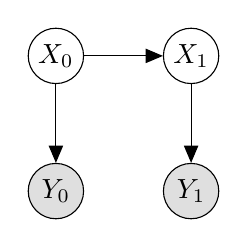
\begin{tikzpicture}

  % Define nodes
  \node[obs] (ya) {$Y_{0}$};
  \node[latent, above=of ya]  (xa) {$X_{0}$};
  \node[obs, right=of ya] (yb) {$Y_{1}$};
  \node[latent, above=of yb, right=of xa]  (xb) {$X_1$};
  
  % Connect the nodes
  \edge {xa} {ya};
  \edge {xa} {xb};
  \edge {xb} {yb};
  
\end{tikzpicture}
\caption{Graphical model used in this chapter.}
\label{fig_linmod}
\end{figure}
Intuitively, this model represents the situation where we are not sure about the state of the world but we can observe some facet of it. At each time step our state changes stochastically according to the transition function. A new observation is (stochastically) generated from our new state. Generally, we attempt to infer the state of the world given the observations. Clearly two new random variables $X_t, Y_t$ are created at each time step.

In this chapter we briefly describe Markov models because they link back to previous work done by the chemical engineering department at the University of Pretoria. We focus on hidden Markov models for the remainder of the chapter because the techniques we develop here generalise to linear latent dynamical systems which we discuss in chapter \ref{sec_inf_lin_mods}. 

\section{Markov models}
A first order Markov model (sometimes called a Markov chain) is shown in Figure \ref{fig_markov_chain}. Using the chain rule for Bayesian networks (Definition \ref{def_chain_rule_bayes}) we can immediately write down the joint probability distribution
\begin{equation}
P(X_{0:T}) = \Pi_{t=0}^T P(X_t|X_{t-1}) \text{ with } P(X_0|X_{-1}) = P(X_0).
\label{eq_markov_chain_joint}
\end{equation}  
\begin{figure}[H] 
\centering
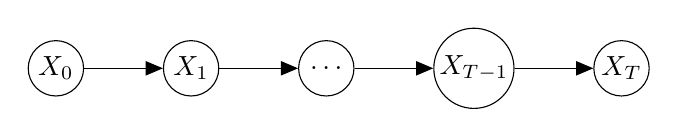
\begin{tikzpicture}

  % Define nodes
  \node[latent]  (xa) {$X_{0}$};
  \node[latent, right=of xa]  (xb) {$X_{1}$};
  \node[latent, right=of xb]  (xc) {$\hdots$};
  \node[latent, right=of xc]  (xd) {$X_{T-1}$};
  \node[latent, right=of xd]  (xe) {$X_{T}$};
  % Connect the nodes
  \edge {xa} {xb};
  \edge {xb} {xc};
  \edge {xc} {xd};
  \edge {xd} {xe};
\end{tikzpicture}
\caption{First order markov chain.}
\label{fig_markov_chain}
\end{figure}
This model describes the forward propagation of a discrete random variable through time. It is interesting to study the marginal distribution of $P(X_T)$ as it evolves through time. By d-separation we know that $X_t \indep X_{0:t-2} | X_{t-1}$. Thus, we only have to marginalise out the previous time step to compute the required distribution 
\begin{equation}
P(X_T) = \sum_{x_{T-1}} P(X_T, x_{T-1}) = \sum_{x_{T-1}} P(x_{T-1})P(X_T|x_{T-1}).
\label{eq_markov_chain_marg}
\end{equation}
Since we know that the transition function is a row stochastic $n \times n$ matrix (the random variable has $n$ discrete states) we can write (\ref{eq_markov_chain_marg}) in vector notation 
\begin{equation}
P(X_t) = \mathbf{p}_t = \mathbf{A}\mathbf{p}_{t-1} = \mathbf{M}^{t-1}\mathbf{p}_1.
\label{eq_markov_chain_marg_vec}
\end{equation}
Note that $P(X_T)$ is a discrete random variable and can thus be expressed as a stochastic column vector i.e. $\sum_i P(x_t=i) = 1$. We have implicitly rewritten (\ref{eq_markov_chain_marg_vec}) in recursive format. Thus, we have a recursive expression for the marginal distribution of $X$. If, as $T \rightarrow \infty$, we have that $\mathbf{p}_{t \rightarrow \infty} = \mathbf{p}_{\infty}$ exists and is independent of $\mathbf{p}_0$ we call $\mathbf{p}_{\infty}$ the equilibrium distribution of the chain. 

We define the stationary distribution, in matrix notation, by \begin{equation}
\mathbf{p}_{\infty} = \mathbf{A}\mathbf{p}_{\infty}.
\label{eq_markov_chain_stationary}
\end{equation}
Recalling the definition of the eigenvalue problem we see that the stationary distribution is just the eigenvector corresponding to the unit eigenvalue of $\mathbf{A}$. While this model may seem simplistic it is the foundation of Google's PageRank algorithm \cite{google}.  Intuitively $\mathbf{p}_\infty$ represents the steady state probability distribution of the random variable $X$ as it is propagated through time by the transition function $A$. See the work in \cite{streicher} for an application specifically geared towards chemical engineering.

\section{Hidden Markov models}
Hidden Markov models extend Markov models by incorporating the observed random variables $(Y_0, Y_1,\hdots)$ as shown in Figure \ref{fig_linmod}. At each time step it is now possible to observe the random variable $Y_t$ which gives more information about the state of $X_t$. We are still in the setting of discrete random variables. It is not necessary to restrict $(Y_0, Y_1,\hdots)$ to be discrete but we do so for the sake of simplicity here. In later chapters we will model both hybrid and purely continuous systems. 

In general a hidden Markov model is just a specific case of the general dynamic Bayesian network class of graphical models. As such we already know that to fully specify the model we only require a prior state distribution $P(X_0)$, the transition probability function $P(X_t|X_{t-1})$, the observation (or sometimes called the emission) probability function $P(Y_t|X_t)$ and the Bayesian network graphs of the initial time step and the next two time steps. We assume that the model's structure repeats at each time step and thus we only require the graph as shown in Figure \ref{fig_linmod}.

We assume that the transition and observation probability functions are stationary. Consequently they may be represented by the row stochastic square matrices $P(x_t=i|x_{t-1}=j) = A$ and $P(y_t=i|x_t=j) = B$. Intuitively this means that the probability of state $x_{t-1}=j$ going to state $x_{t} = i$ is $A_{ij}$. Similarly, $B_{ij}$ is the probability of observing $y_t=i$ if the underlying state is $x_t=j$.

For the purposes of this dissertation we will always assume that the model parameters are known. In section \ref{sec_dbns_lit} the four primary inference techniques were briefly mentioned. We now derive recursive expressions for each inference technique for discrete models of the form shown in Figure \ref{fig_linmod}. The tools and techniques we develop here will be useful in the following chapters. 

\subsection{Filtering}
The goal of filtering is to find $P(X_t|y_{0:t})$: the distribution of the current state given all the past observations. The corresponding graphical model is shown in Figure \ref{fig_linmod_filter_hmm}.
\begin{figure}[H] 
\centering
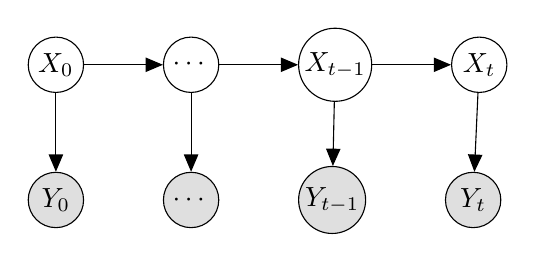
\begin{tikzpicture}

  % Define nodes
  \node[obs] (ya) {$Y_{0}$};
  \node[latent, above=of ya]  (xa) {$X_{0}$};
  \node[obs, right=of ya] (yb) {$\cdots$};
  \node[latent, above=of yb, right=of xa]  (xb) {$\cdots$};
  \node[obs, right=of yb] (yc) {$Y_{t-1}$};
  \node[latent, above=of yc, right=of xb]  (xc) {$X_{t-1}$};  
  \node[obs, right=of yc] (yd) {$Y_t$};
  \node[latent, above=of yd, right=of xc]  (xd) {$X_t$};  
  
  % Connect the nodes
  \edge {xa} {ya};
  \edge {xa} {xb};
  \edge {xb} {yb};
  \edge {xb} {xc};
  \edge {xc} {yc};
  \edge {xc} {xd};
  \edge {xd} {yd};

\end{tikzpicture}
\caption{Filtering graphical model.}
\label{fig_linmod_filter_hmm}
\end{figure}
We start the derivation by noting that $X_{t-1}$ d-separates $X_t$ from $X_{0:t-2}$. Thus $X_{t-1}$ contains all the hidden state information of the system up to and including $t-1$. This is not surprising since we have assumed a first order Markov system. This is why we only marginalise over the reduced state joint $P(X_t, X_{t-1}|y_{0:t})$ in
\begin{equation}
\begin{aligned}
P(X_t| y_{0:t-1}) &= \sum_{x_{t-1}} P(X_t, x_{t-1}| y_{0:t-1})\\
&= \sum_{x_{t-1}} P(x_{t-1}|y_{0:t-1})P(X_t|y_{0:t-1}, x_{t-1})\\  
& = \sum_{x_{t-1}} P(x_{t-1}|y_{0:t-1})P(X_t|x_{t-1}).
\end{aligned}
\label{eq_forward_no_recur}
\end{equation}
The expansion followed from the chain rule of Bayesian networks (Definition \ref{def_chain_rule_bayes}) and the cancellation followed from the conditional independence assumption of the transition function. Next we define $\alpha(X_t) \equiv P(X_t | y_{0:t})$; then
\begin{equation}
\begin{aligned}
\alpha(X_t) &= \frac{P(y_t|X_t, y_{0:t-1})P(X_t|y_{0:t-1})}{P(y_t|y_{0:t-1})} \\
& = \frac{P(y_t|X_t)P(X_t|y_{0:t-1})}{P(y_t|y_{0:t-1})} \\
& = \frac{P(y_t|X_t) \sum_{x_{t-1}} P(x_{t-1}|y_{0:t-1})P(X_t|x_{t-1})}{P(y_t|y_{0:t-1})} \\
& = \frac{P(y_t|X_t) \sum_{x_{t-1}} \alpha(x_{t-1})P(X_t|x_{t-1})}{P(y_t|y_{0:t-1})} \\
\end{aligned}
\label{eq_forward_recur}
\end{equation}
follows from (\ref{eq_forward_no_recur}) and by application of Bayes' theorem (Theorem \ref{thrm_bayes}). It is not actually necessary to calculate $p(y_t|y_{0:t-1})$ as it is only a normalisation constant. We thus have a recursion relation for the filtered posterior distribution $X_t$ with initial condition $\alpha(X_1) = P(X_1, y_1) = P(X_1)P(y_1|X_1)$ by
\begin{equation}
\alpha(X_t) \propto P(y_t|X_t) \sum_{x_{t-1}} \alpha(x_{t-1})P(X_t|x_{t-1}).
\label{eq_forward_approx}
\end{equation}
One often uses logarithms to perform the filter calculations as machine precision errors become a problem for large $t$ due to the multiplication of small fractions. The recursive filtering algorithm we derived is often called the forwards algorithm in literature \cite{barber}.

\subsection{Smoothing}
The goal of smoothing is to find $P(X_t|y_{0:T})$ for $t\leq T$: the distribution of the state at $t$ given all the past and future observations to $T$. The smoothing algorithm we study here is called the parallel smoothing algorithm. The recursion expression we derive is often called the backwards algorithm in literature \cite{murphy1}. The graphical model corresponding to this situation is shown in Figure \ref{fig_linmod_smooth_hmm}.
\begin{figure}[H] 
\centering
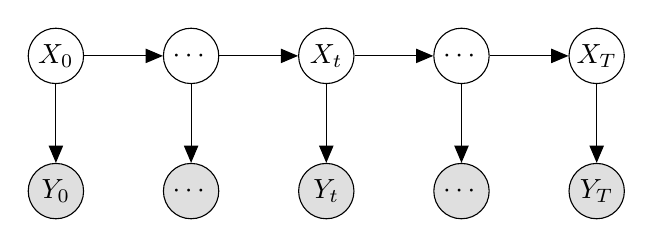
\begin{tikzpicture}

  % Define nodes
  \node[obs] (ya) {$Y_{0}$};
  \node[latent, above=of ya]  (xa) {$X_{0}$};
  \node[obs, right=of ya] (yb) {$\cdots$};
  \node[latent, above=of yb, right=of xa]  (xb) {$\cdots$};
  \node[obs, right=of yb] (yc) {$Y_{t}$};
  \node[latent, above=of yc, right=of xb]  (xc) {$X_{t}$};  
  \node[obs, right=of yc] (yd) {$\cdots$};
  \node[latent, above=of yd, right=of xc]  (xd) {$\cdots$};  
  \node[obs, right=of yd] (ye) {$Y_T$};
  \node[latent, above=of ye, right=of xd]  (xe) {$X_T$};  
  
  % Connect the nodes
  \edge {xa} {ya};
  \edge {xa} {xb};
  \edge {xb} {yb};
  \edge {xb} {xc};
  \edge {xc} {yc};
  \edge {xc} {xd};
  \edge {xd} {yd};
  \edge {xd} {xe};
  \edge {xe} {ye};

\end{tikzpicture}
\caption{Smoothing graphical model.}
\label{fig_linmod_smooth_hmm}
\end{figure}
We start by splitting the joint $P(X_t, y_{0:T}) = P(X_t, y_{0:t})P(y_{t+1:T}|X_t,y_{0:t})$ by the chain rule and using d-separation to reduce it further $P(X_t, y_{0:T}) = P(X_t, y_{0:t})P(y_{t+1:T}|X_t)$. Effectively the last step implies that future observations are independent of past observations given the current state. We defined $\beta(X_t)\equiv P(y_{t+1:T}|X_t)$ and continue
\begin{equation}
\begin{aligned}
P(y_{t:T}|X_{t-1}) &= \sum_{x_t} P(y_t, y_{t+1:T}, x_t|X_{t-1}) \\
&= \sum_{x_t} P(y_{t+1:T}, x_t | X_{t-1})P(y_t| y_{t+1:T}, x_t, X_{t-1}) \\
&= \sum_{x_t} P(y_{t+1:T}, x_t | X_{t-1})P(y_t| x_t) \\
&= \sum_{x_t} P(x_t | X_{t-1})P(y_{t+1:T}| x_t,X_{t-1})P(y_t| x_t) \\
&= \sum_{x_t} P(x_t | X_{t-1})P(y_{t+1:T}| x_t)P(y_t| x_t).
\end{aligned}
\label{eq_backwards_no_recur}
\end{equation}
We have made judicious use of the implied independence assertions (via d-separation) of Figure \ref{fig_linmod}. Making use of the definition of $\beta$ we have
\begin{equation}
\begin{aligned}
&\beta(X_{t-1}) = \sum_{x_t} P(x_t | X_{t-1})\beta(x_t)P(y_t| x_t) \text{ for } 1 \leq t \leq T \\
&\text{with } \beta(X_T) = 1.
\end{aligned}
\label{eq_backwards_recur}
\end{equation}
The recursion initial condition $\beta(X_T) = 1$ stems from Bayes' theorem (Theorem \ref{thrm_bayes}) and the definition of $\alpha$ as illustrated by
\begin{equation}
\begin{aligned}
P(X_T|y_{0:T}) &= \frac{P(X_T, y_{0:T})}{P(y_{0:T})} \\
&= \alpha(X_T) \beta(X_T)\\
&= P(X_T| y_{0:T}) \beta(X_T)\\
&\implies \beta(X_T) = 1.
\end{aligned}
\label{eq_backwards_recur_initial}
\end{equation}
Note that $\beta$ is not a probability function. The smoothed posterior is given by applying Bayes' theorem
\begin{equation}
P(X_t|y_{0:T}) = \frac{\alpha(X_t)\beta(X_t)}{\sum_{x_t}\alpha(x_t)\beta(x_t)}.
\label{eq_smooth}
\end{equation}
Together the $\alpha - \beta$ recursions are called the forwards-backwards algorithm and find extensive use in general purpose exact inference of dynamic Bayesian networks \cite{murphy1}.

Numerical issues may also become problematic due to the multiplication of small positive numbers. In practice it is often necessary to work in the log space to attenuate these problems \cite{barber}. 

\subsection{Viterbi decoding}
The goal of Viterbi decoding is to find $x_{0:T}^* = \underset{x_{0:T}}{\text{arg max }} P(x_{0:T}|y_{0:T})$: finding the most likely sequence of states which best describe the observations by  attempting to find the sequence $x_{0:T}$ such that the joint probability function $P(x_{0:T}, y_{0:T})$ is maximised. This is equivalent to finding $ \underset{x_{0:T}}{\text{arg max }} P(x_{0:T}|y_{0:T})$ because, if one uses the chain rule on the joint, the observations will just be a constant factor. The graphical model used here is similar to that of Figure \ref{fig_linmod_smooth_hmm}.

Intuitively we first attempt to find the maximum of the joint and then determine which sequence of states led to this maximal joint. By using the chain rule for Bayesian networks we can rewrite the joint maximisation problem as
\begin{equation}
\begin{aligned}
\underset{x_{0:T}}{\text{max }} P(x_{0:T}, y_{0:T}) &= \underset{x_{0:T}}{\text{max }} \Pi_{t=1}^T P(y_t|x_t) P(x_t|x_{t-1})\\
&= \left(\underset{x_{0:T-1}}{\text{max }} \Pi_{t=1}^{T-1} P(y_t|x_t) P(x_t|x_{t-1}) \right) \underset{x_{T}}{\text{max }} P(y_T|x_T) P(x_T|x_{T-1}).
\end{aligned}
\label{eq_viterbi_joint}
\end{equation}
Defining $\mu(X_{t-1}) \equiv \underset{x_{t}}{\text{max }} P(y_t|x_t) P(x_t|x_{t-1})$ we can rewrite (\ref{eq_viterbi_joint}) as \begin{equation}
\underset{x_{0:T}}{\text{max }} P(x_{0:T}, y_{0:T}) =\underset{x_{0:T-1}}{\text{max }} \Pi_{t=1}^{T-1} P(y_t|x_t) P(x_t|x_{t-1}) \mu(x_{T-1}).
\label{eq_viterbi_max_factor_mu}
\end{equation}
Thus we have a recursive expression,
\begin{equation}
\begin{aligned}
&\mu(x_{t-1}) = \underset{x_{t}}{\text{max }} P(y_t|x_t) P(x_t|x_{t-1}) \mu(x_t) \text{ for } 2 \leq t \leq T \\
&\text{with } \mu(x_T) = 1, 
\end{aligned}
\label{eq_viterbi_recur}
\end{equation}
to find the value of the joint under the most likely sequence of states given the observations.

The recursive expression in (\ref{eq_viterbi_recur}) implies that the effect of maximising over over the previous time step can be compressed into a message (a function) of the current time step. Effectively we pass theses messages backward in time to find the maximum joint in terms of $x_0$. We then find the state which maximises this joint and pass this message forward.  Continuing in this way we have
\begin{equation}
\begin{aligned}
x_1^* &= \underset{x_{1}}{\text{arg max }}P(y_1|x_1)P(x_1)\mu(x_1) \\
x_2^* &= \underset{x_{2}}{\text{arg max }}P(y_2|x_2)P(x_2|x_1^*)\mu(x_2) \\
&~~\vdots \\
x_t^* &= \underset{x_{t}}{\text{arg max }}P(y_t|x_t)P(x_t|x_{t-1}^*)\mu(x_t).
\end{aligned}
\label{eq_viterbi_recur_forward}
\end{equation}
This algorithm is called the Viterbi algorithm. It is computationally efficient since the optimisations occur only on a single variable. Readers familiar with dynamic programming will recognise that we have effectively performed a variant of dynamic programming in the preceding derivation.

\subsection{Prediction}
The goal of prediction is to find $P(X_{t+1}|y_{0:t})$ and $P(Y_{t+1}|y_{0:t})$: the predicted hidden and observed state given all the previous observations. The one step ahead prediction expression for both the states and observations is derived here. The graphical model corresponding to the state prediction is shown in Figure \ref{fig_linmod_pred_hmm}. 
\begin{figure}[H] 
\centering
\begin{tikzpicture}

  % Define nodes
  \node[obs] (ya) {$Y_{0}$};
  \node[latent, above=of ya]  (xa) {$X_{0}$};
  \node[obs, right=of ya] (yb) {$\cdots$};
  \node[latent, above=of yb, right=of xa]  (xb) {$\cdots$};
  \node[obs, right=of yb] (yc) {$Y_{t}$};
  \node[latent, above=of yc, right=of xb]  (xc) {$X_{t}$};  
  \node[latent, above=of yd, right=of xc]  (xd) {$X_{t+1}$};  
  
  % Connect the nodes
  \edge {xa} {ya};
  \edge {xa} {xb};
  \edge {xb} {yb};
  \edge {xb} {xc};
  \edge {xc} {yc};
  \edge {xc} {xd};
  
\end{tikzpicture}
\caption{State prediction graphical model.}
\label{fig_linmod_pred_hmm}
\end{figure}
We again start by noticing that given all the observations  up to time $t$ the current state d-separates  all previous states. Thus, to infer information about the next state we only need to marginalise out the current state $X_t$. Furthermore, the next state d-separates the next observation from all the previous states. Thus, to infer information about the next observation we additionally only need to marginalise out $X_{t+1}$.

We start with predicting the next state distribution. We have applied the chain rule, the independence assertions and used the definition of $\alpha$ to write
\begin{equation}
\begin{aligned}
P(X_{t+1}|y_{0:t}) &= \sum_{x_t} P(X_{t+1}, x_t|y_{0:t}) \\
&= \sum_{x_t} P(x_t|y_{0:t})P(X_{t+1}|x_t, y_{0:t}) \\
&= \sum_{x_t} P(x_t|y_{0:t})P(X_{t+1}|x_t) \\
&= \sum_{x_t} \alpha(x_t)P(X_{t+1}|x_t).
\end{aligned}
\label{eq_prediction_state}
\end{equation}
Clearly the state prediction uses the filtered state estimate and projects that forward using the transition function. Next we derive the observation prediction. Again we apply the chain rule, use the independence assertions and use the definition of $\alpha$ to write
\begin{equation}
\begin{aligned}
P(Y_{t+1}|y_{0:t}) &= \sum_{x_t, x_{t+1}} P(x_{t+1}, x_t, Y_{t+1}|y_{0:t})\\
&= \sum_{x_t, x_{t+1}} P(x_t|y_{0:t})P(x_{t+1}, Y_{t+1}|y_{0:t}, x_t) \\
&= \sum_{x_t, x_{t+1}} P(x_t|y_{0:t})P(x_{t+1}|y_{0:t}, x_t)P(Y_{t+1}|y_{0:t}, x_t, x_{t+1}) \\
&= \sum_{x_t, x_{t+1}} P(x_t|y_{0:t})P(x_{t+1}|x_t)P(Y_{t+1}|x_{t+1}) \\
&= \sum_{x_t, x_{t+1}} \alpha(x_t)P(x_{t+1}|x_t)P(Y_{t+1}|x_{t+1}).
\end{aligned}
\label{eq_prediction_observation}
\end{equation}
Clearly the observation prediction is just an extension of the state prediction. We effectively just predict the next state and use the observation function to predict the observation distribution.

It is pleasing that the prediction expressions are closely related to each other and effectively only depend on the filtered state estimate and the transition or observation functions. This realisation hold for more general problems and will become important when we consider controlling the system. More on this later.

\section{Burglar localisation problem}
While the focus of this dissertation is not on hidden Markov model type problems it is nevertheless instructive to consider a simple example to build some intuition about inference of random variables. Thus, it is desirable to conduct a numerical experiment using the previously derived inference techniques. The type of problem we consider here is a localisation problem. This type of problem (and its extensions) has many applications in robotics and object tracking.

The problem is taken from Chapter 23 in Barber's book \textit{Bayesian Reasoning and Machine Learning} \cite{barber}. Briefly, it is necessary to infer the location of a burglar in your house given observations (noises) you perceive from an adjoining room. You discretise the room the burglar is in into $n^2$ blocks. The room is then the discrete random variable $X$. You observe two distinct types of noises: creaks and bumps. From the knowledge of your house you know which blocks are likely to creak and which are likely to bump if the burglar is on that block i.e. if the random variable $X$ is in a specific state. This is shown in Figure \ref{fig_burlgar_observations}: a dark block indicates it is likely to emit a noise with probility 0.9 and a light block will emit a noise with probability 0.01 if the burglar is on that block. The noises are independent of each other.
\begin{figure}[H] 
\centering
\includegraphics[scale=0.25]{burglar_observations.pdf}
\caption{Burglar problem observations.}
\label{fig_burlgar_observations}
\end{figure}
The burglar moves up, down, left and right with equal probability where appropriate. See Barber for more details on the example. It is necessary to perform inference to determine the path of the burglar both in real time and with the benefit of hindsight. Applying the inference techniques we developed earlier results in Figure \ref{fig_burglar_inference}. 
\begin{figure}[H] 
\centering
\includegraphics[scale=0.3]{burglar_inference.pdf}
\caption{Burglar problem: filter, smoothing, Viterbi decoding and prediction.}
\label{fig_burglar_inference}
\end{figure}
In this context filtering means we estimate the location of the burglar given all the past observations at the current time step. This inference can be done on-line. Smoothing means we attempt to estimate his position with hindsight given all the observations starting from the first time step and moving forwards. In Viterbi decoding we attempt to estimate the most likely path path of the burglar. Finally the prediction algorithm is self-explanatory.

It is interesting to note that smoothed posterior converges to the filtered posterior near the end of the time window. Reflecting on the expression for smoothing this is not surprising since at $t=T$ the smoothing component of the forwards-backwards algorithm is unity. Therefore we see that the smoothed state estimate converges to the filtered state estimate as $t$ approaches $T$.

It is also interesting to note that the prediction algorithm is very much dependent on the quality of the transition function. The four block pattern readily apparent in the prediction distribution originates from the transition function (the burglar is equally likely to move in any direction). This strongly implies that the closer the transition function is to reality the better our predictions will be.

Finally, it is important to understand the benefit of using this approach as opposed to the exhaustive ``if this then that" approach. Firstly, the latter approach scales exponentially with the number of variables because one would need to fully consider all the possibilities to infer any sort of belief. Secondly, the former approach has an associated probability distribution: the certainty of our inferred belief is automatically quantified e.g. the darker the blocks the more sure we are about our inference. Thus, the techniques we developed make room for uncertainty about the correctness of the answer.

Hidden Markov models are very powerful and have found many uses e.g. speech recognition, object tracking and bio-informatics \cite{barber}. Many extensions of the basic model (see Figure \ref{fig_linmod}) exist which are much more expressive. However, we are interested in modelling and reasoning about continuous random variables. For such applications the hidden Markov model, due to the discrete assumption, is inappropriate. Fortunately, the techniques investigated in this chapter carry over to the continuous case as we will see in chapter \ref{sec_inf_lin_mods}.  

\chapter{CSTR model}
\label{sec_cstr}
In this chapter we introduce the model we will use to illustrate the techniques we develop in this dissertation. The model is a simple continuously stirred tank reactor (CSTR) undergoing an exothermic, irreversible first order reaction where $A \rightarrow B$. A schematic diagram of the reactor is shown in figure \ref{fig_cstr_diagram}. The model is taken from literature \cite{cstrmodel}.
\begin{figure}[H] 
\centering
\includegraphics[scale=0.8]{cstr_diagram.pdf}
\caption{Diagram of a simple CSTR where the heat added to system is the only manipulated variable.}
\label{fig_cstr_diagram}
\end{figure}
The state space equations describing the reactor are 
\begin{equation}
\begin{aligned}
\dot{C_A} &= f(C_A, T_R) =  \frac{F}{V}\left( C_{A0}-C_A \right) - k_0e^{\frac{-E}{RT_R}}C_A \\
\dot{T_R} &= g(C_A, T_R) = \frac{F}{V}\left(T_{A0}-T_R\right) + \frac{-\triangle H}{\rho C_p}k_0e^{\frac{-E}{RT_R}}C_A + \frac{Q}{\rho C_p V}
\end{aligned}
\label{eq_cstrmodel}
\end{equation}
with parameters shown in table \ref{tab_params}. The meaning of the variables is what one would expect from an intuitive understanding: $C_A$ is the concentration of species $A$, $T_R$ is the temperature of the CSTR and $Q$ is the heat added (or removed for negative $Q$) from the CSTR.
\begin{table}[H]
\begin{center}
\begin{tabular}{c c c c}
\hline
$V$ & $~5.0~m^3$ & $R$ & $~8.314~\frac{kJ}{kmol.K}$ \\
$C_{A0}$ & $~1.0~\frac{kmol}{m^3}$ &$T_{A0}$ & $~310~K$ \\
$\triangle H$ & $~-4.78\times 10^{4}~\frac{kJ}{kmol}$ & $k_{0}$ & $~72\times 10^{7}~\frac{1}{min}$ \\
$E$ & $~8.314\times 10^4~\frac{kJ}{kmol}$ & $C_{p}$ & $~0.239~\frac{kJ}{kg.K}$ \\
$\rho$ & $~1000~\frac{kg}{m^3}$ & 
$F$ & $~100\times 10^{-3}~\frac{m^3}{min}$ \\
\hline
\end{tabular}
\caption{CSTR parameters}
\label{tab_params}
\end{center}
\end{table}
The CSTR model is a familiar control example. Similar models may be found in \cite{du}, \cite{cervantes}, \cite{pan} and~\cite{yazdi}. We use this model because it is low dimensional yet complex enough to illustrate the principles we investigate. CSTR models are also very popular examples to illustrate control techniques because they invariably have nonlinear dynamics and multiple steady states. Note that we have increased the volume of the reactor and reduced the rate constant from the reactor we quoted in literature. This is primarily to adjust the time scale of the transient response to be in the order of minutes and not milliseconds when moving to high temperature regions of operation.

\section{Qualitative analysis}
In this section we use standard mathematical tools, as found in \cite{edwardsandpenny}, to analyse the qualitative behaviour of the CSTR. By inspecting (\ref{eq_cstrmodel}) we see that the model is coupled and nonlinear. By solving
\begin{equation}
\begin{aligned}
0 &= \frac{F}{V}\left( C_{A0}-C_A \right) - k_0e^{\frac{-E}{RT_R}}C_A \\
0 &= \frac{F}{V}\left(T_{A0}-T_A\right) + \frac{-\triangle H}{\rho C_p}k_0e^{\frac{-E}{RT_R}}C_A + \frac{Q}{\rho C_p V}
\end{aligned}
\label{eq_cstr_statpoints}
\end{equation}
we see that for nominal operating conditions ($Q = 0$) there exist 3 operating points (critical points) as shown in table \ref{tab_nominalstats}.
\begin{table}[H]
\begin{center}
\begin{tabular}{c c c c}
\hline
Critical Point & $C_A$ & $T_R$ & Stability\\
\hline
$\left(C_A^1, T_R^1\right)$ & 0.0097 & 508 & Stable Improper Node\\
$\left(C_A^2, T_R^2\right)$ & 0.4893 & 412 & Unstable Saddle Point \\
$\left(C_A^3, T_R^3 \right)$ & 0.9996 & 310 & Stable Improper Node \\
\hline
\end{tabular}
\caption{Nominal operating points for  the CSTR}
\label{tab_nominalstats}
\end{center}
\end{table}
The stability of the operating points were found by linearising (\ref{eq_cstrmodel}) and computing the eigenvalues of the jacobian,
\begin{equation}
J(C_A, T_R) = \begin{pmatrix}
-\frac{F}{V} - k_0e^{\frac{-E}{RT_R}} & - k_0e^{\frac{-E}{RT_R}}C_A\left(\frac{E}{RT_R^2}\right) \\
\frac{-\triangle H}{\rho C_p}k_0e^{\frac{-E}{RT_R}} & -\frac{F}{V} + \frac{-\triangle H}{\rho C_p}k_0e^{\frac{-E}{RT_R}}C_A\left(\frac{E}{RT_R^2}\right)
\end{pmatrix},
\label{eq_jacobian}
\end{equation}
at each critical point. In figure \ref{fig_cstr_op_curve} we see the operating curve for the CSTR. The curve resembles the classical CSTR operating curve with all the associated potential control complexity e.g. it is possible for one set of control inputs to result in two stable operating points. This occurs due to the two stable critical points (for $Q\in [-906, 1145]$) of the system and is called input multiplicity \cite{luyben}. 

Also note that the obvious bifurcation parameter for this system is the heat input $Q$. For $Q = -906$ kJ/min we see that we no longer have three critical points but only two, and for $Q < -906$ kJ/min we only have one critical point. Likewise, for $Q = 1145$ kJ/min we see that we only have two critical points and for $Q > 1145$ kJ/min we only have one critical point. The stability of these points are shown in table \ref{tab_bifurc}.  
\begin{figure}[H] 
\centering
\includegraphics[width=\textwidth]{cstr_model_op_curve.pdf}
\caption{CSTR operating curve with different input curves. Nominal operating conditions are $Q=0$ kJ/min.}
\label{fig_cstr_op_curve}
\end{figure}
\begin{table}[H]
\begin{center}
\begin{tabular}{c c c c}
\hline
Heat Input & $C_A$ & $T_R$ & Stability\\
\hline
$Q = -906$ kJ/min & 0.1089 & 450 & Stable Improper Node\\
$Q = -906$ kJ/min & 0.9999 & 272 & Stable Improper Node \\
\hline
$Q < -906$ kJ/min & $\backsim$ & $\backsim$ & Stable Improper Node \\
\hline
$Q = 1145$ kJ/min & 0.0017 & 558 & Stable Improper Node\\
$Q = 1145$ kJ/min & 0.9263 & 373 & Stable Improper Node \\
\hline
$Q > 1145$ kJ/min & $\backsim$ & $\backsim$ & Stable Improper Node \\
\hline
\end{tabular}
\caption{Bifurcation analysis of the CSTR at different heat input values. The $\backsim$ notation indicates that the operating point depends on the precise value of $Q$.}
\label{tab_bifurc}
\end{center}
\end{table}
The (potentially) multiple stable critical points separated by the unstable critical point makes control of this system challenging.    

\section{Nonlinear model}
In this section we evaluate the transient response of the CSTR. The nonlinear differential equation shown in (\ref{eq_cstrmodel}) is intractably difficult to solve analytically. For this reason we will use a numerical method, specifically the Runge-Kutta method \cite{edwardsandpenny}, to simulate the transient response. We chose the Runge-Kutta method because it is an explicit, fourth order accurate method which is easy to implement.

For completeness we show the method here. Suppose we have an autonomous ordinary differential equation,
\begin{equation}
\begin{aligned}
&\dot{x}(t) = f(x(t)) \\
&\text{with } x(t) = x_a \text{ for } t=t_a,
\end{aligned}
\label{eq_ode}
\end{equation}
and we require its solution over $[t_a, t_b]$. This is an initial value problem; for the sake of brevity we assume that a unique solution always exists. Furthermore, suppose we discretise the time domain such that $[t_a, t_b] = [t_0=t_a, t_1= t_a+ h, t_2=t_a+ 2h,...,t_T = t_b]$. Then the scheme
\begin{equation}
\begin{aligned}
x_{t+1} &= x_{t} + \frac{h}{6}\left(k_1 + 2k_2 + 2k_3 +k4\right) \\
k_1 &= f(x_t) \\
k_2 &= f(x_t + \frac{h}{2}k_1) \\
k_3 &= f(x_t+ \frac{h}{2}k_2) \\
k_4 &= f(x_t+ hk_3) \\
\end{aligned}
\label{eq_rk}
\end{equation}
is called the Runge-Kutta method. For sufficiently small time steps, $h$, the method is stable and convergent.
  
By applying the Runge-Kutta method to the CSTR we have figures \ref{fig_cstr_nl_1} and \ref{fig_cstr_nl_2}. It is clear that the dynamics are faster (almost two orders of magnitude) when moving to the higher temperature operating point than they are when moving to the lower temperature operating point. The impact of the nonlinear kinetics is seen here. 
\begin{figure}[H] 
\centering
\includegraphics[width=\textwidth]{cstr_nl_1.pdf}
\caption{Transient response of the CSTR under nominal operating conditions with initial condition $(0.5, 450)$ and $h=0.1$.}
\label{fig_cstr_nl_1}
\end{figure}
\begin{figure}[H] 
\centering
\includegraphics[width=\textwidth]{cstr_nl_2.pdf}
\caption{Transient response of the CSTR under nominal operating conditions with initial condition $(0.5, 400)$ and $h=0.1$.}
\label{fig_cstr_nl_2}
\end{figure}
It is often desirable to linearise a nonlinear system about some point, usually the operating point, to simplify the model. Computationally this is advantageous because linear techniques (e.g. linear optimisation) are usually significantly faster than nonlinear techniques. Practically linearisation is only valid in a small region around the point of linearisation. If the system moves away from the linearisation point the linear approximation can become grossly inaccurate. 

Based on figure \ref{fig_cstr_nl_1}, where the dynamics are fast, we can venture a guess that linearisation will be a bad approximation, except for a very small time period, of plant behaviour because the states will rapidly move away from the point of linearisation.

On the other hand, based on figure \ref{fig_cstr_nl_2}, we can venture a guess that linearisation will be a fair approximation of plant behaviour for a meaningful period of time because the dynamics are slow.

\section{Linearised models}
Linear approximations used for modelling and control are very common both in practice and literature \cite{luyben}. Furthermore, the approach of using multiple piecewise affine (linear) functions for control, based on linearisation around critical points, has also been investigated in literature \cite{du}, \cite{kvasnica}. Typically the state domain is discretised into regimes and the linear approximation of the model in each regime is used for control. We will also use linear models for the purposes of control.  It is therefore prudent to investigate linearisation techniques.

First we present a linearisation technique. Consider an arbitrary point in the state space $(C_A^*, T_R^*)$. Then
\begin{equation}
\begin{pmatrix}
\dot{C_A} \\ \dot{T_R}
\end{pmatrix} = \begin{pmatrix}
f(C_A^*, T_R^*) \\ g(C_A^*, T_R^*)
\end{pmatrix} + J(C_A^*, T_R^*) \left( \begin{pmatrix}
C_A \\ T_R
\end{pmatrix} - \begin{pmatrix}
C_A^* \\ T_R^* 
\end{pmatrix}\right)
\label{eq_lin}
\end{equation}
is the general linearised model around $(C_A^*, T_R^*)$ using the notation of (\ref{eq_cstrmodel}). It is often desirable to change the variables such that (\ref{eq_lin}) has no constant terms. This change of variables, which holds even if the linearisation point is not a critical point of the model, is 
\begin{equation}
\begin{pmatrix}
\tilde{C}_A \\ \tilde{T}_R
\end{pmatrix} = \begin{pmatrix}
C_A \\ T_R
\end{pmatrix} - J(C_A^*, T_R^*)^{-1}\left(J(C_A^*, T_R^*)\begin{pmatrix}
C_A^* \\ T_R^* 
\end{pmatrix} - \begin{pmatrix}
f(C_A^*, T_R^*) \\ g(C_A^*, T_R^*)
\end{pmatrix}_{Q=0} \right).
\label{eq_change_vars}
\end{equation}
We then have
\begin{equation}
\frac{d}{dx}\begin{pmatrix}
\tilde{C_A} \\ \tilde{T_R}
\end{pmatrix} =  J(C_A^*, T_R^*)\begin{pmatrix}
\tilde{C}_A \\ \tilde{T}_R
\end{pmatrix} + B(C_A^*, T_R^*)Q.
\label{eq_lin2}
\end{equation}
Note that the input term $B$ originates from $\begin{pmatrix}
f(C_A^*, T_R^*) \\ g(C_A^*, T_R^*)
\end{pmatrix}$ and in (\ref{eq_change_vars}) we specifically set it to zero so that it is not removed. We now use the bilinear transform (also known as Tustin's transform) to convert (\ref{eq_lin2}) into the discrete equation
\begin{equation}
\begin{pmatrix}
\tilde{C}_A \\ \tilde{T}_R
\end{pmatrix}_{t+1} = A(C_A^*, T_R^*) \begin{pmatrix}
\tilde{C}_A \\ \tilde{T}_R
\end{pmatrix}_{t} + B(C_A^*, T_R^*)Q. 
\label{eq_rkss}
\end{equation}
Observe that (\ref{eq_rkss}) implicitly depends on the sampling time. Recall that $Q$ is the heat input to the system. Note that we need to add back the offset we removed in the change of variables step (\ref{eq_change_vars}) when we want to physically interpret the results of applying (\ref{eq_rkss}).

Next we briefly investigate the accuracy of the linear models. In all the subsequent figures the first subplot illustrates the accuracy of the linear model if the initial value is close to the point of linearisation and the second subplot illustrates the accuracy when the initial value is further away from the point of linearisation.

Figure \ref{fig_cstr_lin_1} shows the state space response of the linear model which was linearised around the high temperature, low concentration stable operating point $(C_A^1,T_R^1)$ as defined in table \ref{tab_nominalstats}.
\begin{figure}[H] 
\centering
\includegraphics[width=\textwidth]{cstr_lin_1.pdf}
\caption{State space response of the CSTR under nominal operating conditions linearised around $(C_A^1,T_R^1)$ with different initial conditions. The dot indicates where the simulation started and the cross where it finished. Total simulation time was 30 seconds.}
\label{fig_cstr_lin_1}
\end{figure}
We see that the linear approximation is quite accurate if the initial condition is close to the linearisation point (as expected). If the initial condition is further away the approximation is less accurate.

In figure \ref{fig_cstr_lin_2} we see the state space response of the CSTR using the linear model linearised around the unstable operating point. Clearly this approximation is less accurate because the system tend to move away from operating point rather than towards it. 
\begin{figure}[H] 
\centering
\includegraphics[width=\textwidth]{cstr_lin_2.pdf}
\caption{State space response of the CSTR under nominal operating conditions linearised around $(C_A^2,T_R^2)$ with different initial conditions. The dot indicates where the simulation started and the cross where it finished. Total simulation time was 5 minutes.}
\label{fig_cstr_lin_2}
\end{figure}
If we want to use the linear model around the unstable operating point we will need to effect control to keep it within some region where the model is accurate.

In figure \ref{fig_cstr_lin_3} we have the state space response of the CSTR under nominal conditions, like before, except that we have now linearised around the low temperature high concentration operating point. 
\begin{figure}[H] 
\centering
\includegraphics[width=\textwidth]{cstr_lin_3.pdf}
\caption{State space response of the CSTR under nominal operating conditions linearised around $(C_A^3,T_R^3)$ with different initial conditions. The dot indicates where the simulation started and the cross where it finished. Total simulation time was 50 minutes.}
\label{fig_cstr_lin_3}
\end{figure}
Like figure \ref{fig_cstr_lin_1}, the linear model is quite accurate. The slow dynamics and stability of the operating point cause this desirable behaviour.

Based on the general linearisation formula in (\ref{eq_lin}) there is no reason why one cannot linearise about an arbitrary point in the state space. It stands to reason that the more linear models at different linearisation points one has, the better one will be able to model the reactor. By selecting a model to use based on some metric (taking into account the current observation) it is reasonable to suppose that one will be able to model the system more accurately than if only one linear model was available. In part \ref{part_three} we take this idea further.

However, in part \ref{part_two} we restrict our attention to systems where one linear model is sufficient for our purposes.  
\documentclass[../masters.tex]{subfiles}

\begin{document}
\graphicspath{{./imgs/}{../imgs/}} %look for images

\section{Linear Models}
In this section we consider probabilistic graphical models of the form shown in Figure \ref{fig_linmod}. Firstly we investigate a model where the states ($X$) and observations ($Y$) are discrete. Models of this form are classically called Hidden Markov Models (HMMs). Secondly we generalise the model to include continuous states and observations. Models of this form are called Latent Linear Dynamical Systems (the famous Kalman Filter model falls into this category).
\begin{figure}[H] 
\centering
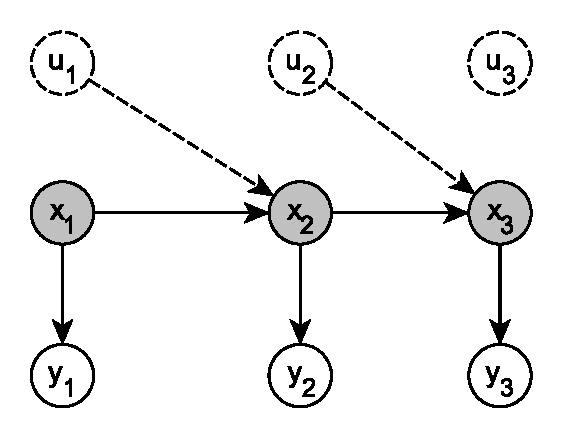
\includegraphics[scale=1.0]{linear_model.pdf}
\caption{Linear Graphical Model}
\label{fig_linmod}
\end{figure}
Intuitively, this model represents the situation where we are not sure about the state of the world but we have some idea represented by the prior $P(X_1)$. At each time step our state changes according to the transition function and we attempt to, amongst other things, infer the new state, perhaps given some observations related to the past and current state.

\subsection{Discrete Models}
In this section we briefly describe Markov Models because they link back to previous work done by the Chemical Engineering Department at the University of Pretoria. We focus on Hidden Markov Models for the remainder of the section because they generalise to Latent Linear Dynamical Systems. 

\subsubsection{Markov Models}
A first order Markov Model (sometimes called a Markov Chain) is shown in Figure \ref{fig_markov_chain}. Using the chain rule for Bayesian Networks we can immediately write down the joint probability distribution as shown in (\ref{eq_markov_chain_joint}).
\begin{equation}
P(X_{1:T}) = \Pi_{t=1}^T P(X_t|X_{t-1}) \text{ with } P(X_1|X_{-1}) = P(X_1)
\label{eq_markov_chain_joint}
\end{equation}  
\begin{figure}[H] 
\centering
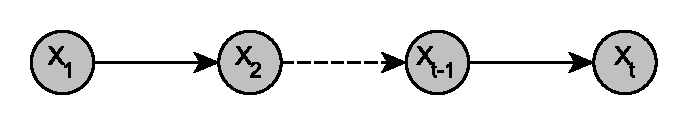
\includegraphics[scale=1.0]{markov_chain.pdf}
\caption{First Order Markov Chain}
\label{fig_markov_chain}
\end{figure}
This model describes the forward propagation of a discrete random variable through time. It is interesting to study the marginal distribution of $P(X_t)$ as it evolves through time. By d-separation we know that $X_t \indep X_{1:t-2} | X_t$. Thus, we only have to marginalise out the previous time step to compute the required distribution as shown in (\ref{eq_markov_chain_marg}).
\begin{equation}
P(X_t) = \sum_{x_{t-1}} P(X_t, x_{t-1}) = \sum_{x_{t-1}} P(x_{t-1})P(X_t|x_{t-1})
\label{eq_markov_chain_marg}
\end{equation}
Since we know that the transition function is a row stochastic $n \times n$ matrix (the random variable has $n$ discrete states) we can write (\ref{eq_markov_chain_marg}) in vector notation (\ref{eq_markov_chain_marg_vec}).
\begin{equation}
P(X_t) = \mathbf{p}_t = \mathbf{A}\mathbf{p}_{t-1} = \mathbf{M}^{t-1}\mathbf{p}_1
\label{eq_markov_chain_marg_vec}
\end{equation}
We have implicitly rewritten (\ref{eq_markov_chain_marg_vec}) in recursive format. Thus we have a recursive expression for the marginal distribution of $X$. If, as $t \rightarrow \infty$, we have that $\mathbf{p}_{t \rightarrow \infty} = \mathbf{p}_{\infty}$ is independent of $\mathbf{p}_1$ we call $\mathbf{p}_{\infty}$ the equilibrium distribution of the chain. 

We define the stationary distribution, in matrix notation, by (\ref{eq_markov_chain_stationary}).
\begin{equation}
\mathbf{p}_{\infty} = \mathbf{A}\mathbf{p}_{\infty}
\label{eq_markov_chain_stationary}
\end{equation}
Recalling the definition of the eigenvalue problem we see that the stationary distribution is just the eigenvector corresponding to the unit eigenvalue of $\mathbf{A}$. While this model may seem simplistic it is the foundation of Google's PageRank algorithm \cite{google}.  Intuitively $\mathbf{p}_\infty$ represents the steady state distribution of the random variable $X$ as it is propagated through time by the transition function $A$.

\subsubsection{Hidden Markov Models}
Hidden Markov Models extend Markov Models by incorporating the observed random variable $Y$ as shown in Figure \ref{fig_linmod}. At each time step it is now possible to observe some value $y_t$ which gives more information about the state of $X_t$. We are still in the setting of discrete random variables. It is not necessary to restrict $Y$ to be discrete but we do so for the sake of simplicity here. In later sections we will model hybrid and purely continuous systems. 

In general a Hidden Markov Model is just a specific case of the general Dynamic Bayesian Network class of graphical models. As such we already know that to fully specify the model we only require a prior state distribution $P(X_1)$, the transition probability function $P(X_t|X_{t-1})$, the observation or emission probability function $P(Y_t|X_t)$ and the Bayesian Network graphs of the initial time step and the next two time steps. We assume that the model's structure repeats at each time step and thus we only require the graph as shown in Figure \ref{fig_linmod}. 

We assume that the transition and observation probability functions are stationary. Consequently they may be represented by the row stochastic square matrices $P(x_t=i|x_{t-1}=j) = \mathbf{A}$ and $P(y_t=i|x_t=j) = \mathbf{B}$. Intuitively this means that the probability of state $x_{t-1}=j$ going to state $x_{t} = i$ is $A_{ij}$. Similarly, $B_{ij}$ is the probability of observing $y_t=i$ if the underlying state is $x_t=j$.

For the purposes of this dissertation we will always assume that the model parameters are known. In the previous section the four primary inference techniques were briefly mentioned. We now derive recursive expressions for each inference technique for discrete models of the form of Figure \ref{fig_linmod}. In the next section we show that these derivations also hold for the continuous case with some minor modifications.

\textbf{Filter:} $P(X_t|y_{1:t})$\\
We start the derivation by noting that $X_{t-1}$ d-separates $X_t$ from $X_{1:t-2}$. Thus $X_{t-1}$ contains all the hidden state information of the system up to and including $t-1$ - this is not surprising since we have assumed a first order Markov system. This is why we consider the reduced state joint $P(X_t, X_{t-1},y_{1:t})$.
\begin{equation}
\begin{aligned}
P(X_t, y_{1:t}) &= \sum_{x_{t-1}} P(X_t, x_{t-1}, v_{1:t-1},v_t)\\
&= \sum_{x_{t-1}} P(y_{1:t-1}, x_{t-1})P(X_t, y_t|y_{1:t}, x_{t-1})\\  & = \sum_{x_{t-1}} P(y_{1:t-1}, x_{t-1})P(X_t|y_{1:t}, x_{t-1})P(y_t|X_t,y_{1:t}, x_{t-1}) \\
&= \sum_{x_{t-1}} P(y_{1:t-1}, x_{t-1})P(X_t|x_{t-1})P(y_t|X_t) \\
\end{aligned}
\label{eq_forward_no_recur}
\end{equation}
Where the expansions followed from the chain rule and the cancellations followed from the conditional independence assumptions of the transition and observation functions. Now we define $\alpha(X_t)=P(X_t,y_{1:t})$. Then (\ref{eq_forward_recur}) follows from (\ref{eq_forward_no_recur}).
\begin{equation}
\begin{aligned}
&\alpha(X_t) = P(y_t|X_t)\sum_{x_{t-1}}P(X_t|X_{t-1})\alpha(X_{t-1}) \text{ for } t>1\\
&\text{with } \alpha(X_1) = P(X_1, y_1) = P(X_1)P(y_1|X_1)
\end{aligned}
\label{eq_forward_recur}
\end{equation}
Clearly we have just derived a recursive expression for the joint distribution $P(X_t, y_{1:t})$. This recursion is called forward recursion in graphical model literature \cite{barber}. To complete our task of estimating $P(X_t|y_{1:t})$ we recall Bayes' Theorem as shown in (\ref{eq_forward_filter}).
\begin{equation}
P(X_t|y_{1:t}) = \frac{P(X_t, y_{1:t})}{P(y_{1:t})} = \frac{\alpha(X_t)}{P(y_{1:t})}
\label{eq_forward_filter}
\end{equation}
Noting that $P(y_{1:t})$ is just a normalisation constant it suffices to normalise $\alpha(X_t)$ to find the filtered distribution of $X_t$ given the observations $y_{1:t})$. One often uses logarithms to perform the filter calculations as machine precision errors become a problem for large $t$ due to the multiplication of small fractions \cite{barber}.

\textbf{Smoothing:} $P(X_t|y_{1:T})$ for $t<T$\\
The smoothing algorithm we study here is called the parallel smoothing algorithm and is often called the Backwards algorithm in literature \cite{murphy1}.


\textbf{Viterbi Decoding:} \\

\textbf{Prediction:} \\


\textbf{Burglar Localisation Problem} \\
xgd
\begin{figure}[H] 
\centering
\includegraphics[scale=0.30]{burglar_inference.pdf}
\caption{Burglar Problem: Filter, Smoothing and Viterbi Decoding}
\label{fig_burglar_inference}
\end{figure}

\begin{figure}[H] 
\centering
\includegraphics[scale=0.30]{burglar_prediction.pdf}
\caption{Burglar Problem: Prediction}
\label{fig_burlgar_prediction}
\end{figure}


\subsection{Continuous Models}
In the previous

\bibliographystyle{plain}
\bibliography{research}

\end{document}
\documentclass[../masters.tex]{subfiles}

\begin{document}
\graphicspath{{./imgs/}{../imgs/}} %look for images

\section{Nonlinear Models}
In this section we still consider probabilistic graphical models of the form shown in Figure \ref{fig_linmod}. The variables retain their meaning as before but we generalise the model by dropping the linearity assumption. Unfortunately, this generalisation, although allowing us to expand our investigation to a much more expressive class of models, makes closed form solutions to the inference problem intractable in general.   
\begin{figure}[H] 
\centering
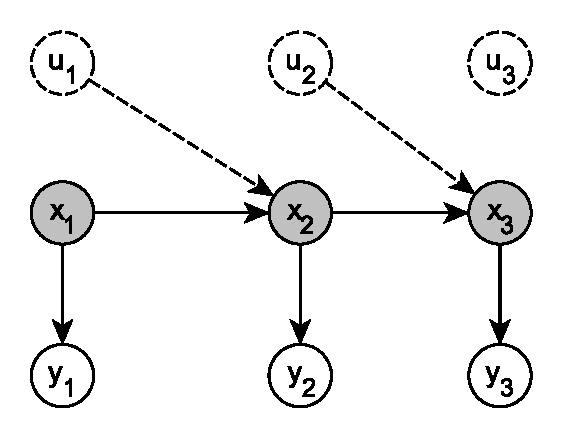
\includegraphics[scale=1.0]{linear_model.pdf}
\caption{Graphical model of this section}
\label{fig_linmod}
\end{figure}
We again assume that the transition and emission functions are time invariant. The state space model is now of the form (\ref{eq_statespace}).
\begin{equation}
\begin{aligned}
x_{t+1} &= f(x_t, u_t, w_{t+1}) \\
y_{t+1} &= g(x_{t+1}, v_{t+1})
\end{aligned}
\label{eq_statespace}
\end{equation}
Note that we make no assumption about the functional form of the noise terms $w_t,v_t$. In practice it is customary to assume that they have zero mean but otherwise are not restricted.

\subsection{Sequential Monte Carlo Methods}
Many approximate inference techniques exist in literature but we shall focus only on Sequential Monte Carlo (SMC) methods because it is simple to implement and generalises well (and easily) to more complex graphical models. 

SMC methods are a general class of Monte Carlo methods which sample sequentially from the growing target distribution $\pi_t(x_{1:t})$. By only requiring that $\gamma_t$ be known point-wise we have the framework of SMC methods as shown in (\ref{eq_SMC1}). Note that $Z_t$ is some normalisation constant \cite{pftut}.
\begin{equation}
\begin{aligned}
\pi_t(x_{1:t}) &= \frac{\gamma_t(x_{1:t})}{Z_t} \\
Z_t &= \int_{x_{1:t}} \gamma_t(x_{1:t})
\end{aligned}
\label{eq_SMC1}
\end{equation} 
For example, in the context of filtering we have that $\gamma_t(x_{1:t}) = p(x_{1:t},y_{1:t})$ and $Z_t = p(y_{1:t})$ so that $\pi_t(x_{1:t}) = p(x_{1:t}|y_{1:t})$. 

It is possible to approximate the distribution $\pi_t(x_{1:t})$ by drawing $N$ samples $X_{1:t}^i \backsim \pi_t(x_{1:t})$ and using the Monte Carlo method to find the approximation $\hat{\pi}_t(x_{1:t})$ as shown in (\ref{eq_SMC2}).
\begin{equation}
\hat{\pi}_t(x_{1:t}) = \frac{1}{N}\sum_{i=1}^N \delta(X^i_{1:t}, x_{1:t})
\label{eq_SMC2}
\end{equation}
We denote the Dirac Delta function of $x$ with mass located at $x_0$ by $\delta(x_0,x)$. It is easy to approximate the marginal $\pi_t(x_{t})$ as shown in (\ref{eq_SMC3}).
\begin{equation}
\hat{\pi}_t(x_{t}) = \frac{1}{N}\sum_{i=1}^N \delta(X^i_{t}, x_{t})
\label{eq_SMC3}
\end{equation}
It can be shown that the variance of the approximation error of $\pi_t$ decreases at rate $\mathcal{O}(\frac{1}{N})$. Unfortunately there are two significant drawbacks to the Monte Carlo approximation. The first is that often we cannot sample from $\pi_t(x_{1:t})$ directly and the second is that even if we could it is often computationally prohibitive. 

We use the Importance Sampling method to address the first problem. We do this by introducing an importance (sometimes called proposal) density $q_t(x_{1:t})$ such that $\pi_t(x_{1:t}) > 0 \implies q_t(x_{1:t}) > 0$. By substituting this into the SMC framework (\ref{eq_SMC1}) we have (\ref{eq_SMC4}).
\begin{equation}
\begin{aligned}
\pi_t(x_{1:t}) &= \frac{w_t(x_{1:t})q_t(x_{1:t})}{Z_t} \\
Z_t &= \int_{x_{1:t}} w_t(x_{1:t})q_t(x_{1:t})
\end{aligned}
\label{eq_SMC4}
\end{equation} 
Where we have defined the unnormalised weight function $w_t(x_{1:t}) = \frac{\gamma_t(x_{1:t})}{q_t(x_{1:t})}$. It is possible, for example, to set $q_t$ to a multivariate Gaussian which is easy to sample from. By drawing $N$ samples $X_{1:t}^i \backsim q_t(x_{1:t})$ and using (\ref{eq_SMC4}) we have (\ref{eq_SMC5}). 
\begin{equation}
\begin{aligned}
\hat{\pi}_t(x_{1:t}) &= \frac{1}{N}\sum_{i=1}^N W_t^i\delta(X^i_{1:t}, x_{1:t}) \\
\hat{Z}_t &= \frac{1}{N}\sum_{i=1}^N w_t(X^i_{1:t}) \\
W^i_t &= \frac{w_t(X^i_{1:t})}{\sum_{i=1}^N w_t(X^i_{1:t})}
\end{aligned}
\label{eq_SMC5}
\end{equation}
Now we will attempt to modify the Importance Sampling method to address the second problem of computational cost incurred by the sampling routine. 

We do this by selecting an importance/proposal distribution which factorises according to $q_t(x_{1:t}) = q_{t-1}(x_{1:t-1})q_t(x_{t}|x_{1:t-1}) = q_1(x_1) \Pi_{k=2}^t q_k(x_k|x_{1:k-1})$. In this way we only need to sample sequentially at each time step: at time $t=1$ we sample $X_1^i \backsim q_1(x_1)$, at time $t=2$ we sample $X_{2}^i \backsim q_2(x_2|x_1)$ and so we build up $X^i_{1:t} \backsim q_t(x_{1:t})$ factor by factor.

The weights can be written in the form (\ref{eq_SMC6}).
\begin{equation}
\begin{aligned}
w_t(x_{1:t}) &= \frac{\gamma_t(x_{1:t})}{q_t(x_{1:t})} \\
&= \frac{\gamma_{t-1}(x_{1:t-1})}{q_{t-1}(x_{1:t-1})}\frac{\gamma_t(x_{1:t})}{\gamma_{t-1}(x_{1:t-1})q_t(x_t|x_{1:t-1})} \\
&= w_{t-1}(x_{1:t-1})\alpha_t(x_{1:t-1}) \\
&= w_1(x_1)\Pi_{k=2}^t \alpha_k(x_{1:k})
\end{aligned}
\label{eq_SMC6}
\end{equation}
Thus, at any time $t$ we can obtain the estimates $\hat{\pi}_t(x_{1:t})$ and $Z_t$. The major limitation of this approach is that the variance of the resulting estimates typically increases exponentially with $t$ \cite{pftut}. 

We overcome this problem by resampling and thus introduce the Sequential Importance Resampling (SIR) method. So far we have a set of weighted samples generated from $q_t(x_{1:t})$ which builds the approximation $\hat{\pi}_t(x_{1:t})$. However, sampling directly from $\hat{\pi}_t(x_{1:t})$ does not approximate $\pi_t(x_{1:t})$. To obtain an approximate distribution of $\pi_t(x_{1:t})$ we need to sample from the weighted distribution $\hat{\pi}_t(x_{1:t})$. This is called resampling because we are sampling from a sampled distribution. Many techniques exist to perform this step efficiently. The crudest and most widely used one is to simply use the discrete multinomial distribution based on $W^i_{1:t}$ to draw samples from $\hat{\pi}_t(x_{1:t})$ \cite{pftut}. 

The benefit of resampling is that it allows us to remove particles with low weight and thus keeps the variance of the estimate in check. We are finally ready to consider the general SIR  algorithm:

For $t=1$:
\begin{enumerate}
\item
Sample $X^i_1 \backsim q_1(x_1)$.
\item
Compute the weights $w_1(X_1)$ and $W^i_1 \propto w_1(X^i_1)$.
\item
Resample $(W^i_1, X^i_1)$ to obtain $N$ equally weighted particles $(\frac{1}{N}, \bar{X}^i_1)$.
\end{enumerate}
For $t \geq 2$:
\begin{enumerate}
\item
Sample $X^i_t \backsim q_t(x_t|\bar{X}^i_{1:t-1})$ and set ${X}^i_{1:t} \leftarrow (\bar{X}^i_{1:t-1}, X^i_t)$ .
\item
Compute the weights $\alpha_t(X^i_{1:t})$ and $W^i_t \propto \alpha_t(X^i_{1:t})$.
\item
Resample $(W^i_t, X^i_{1:t})$ to obtain $N$ equally weighted particles $(\frac{1}{N}, \bar{X}^i_{1:t})$.
\end{enumerate}
At any time $t$ we have two approximations for $\pi(x_{1:t})$ as shown in (\ref{eq_smc_algo}).
\begin{equation}
\begin{aligned}
\hat{\pi}(x_{1:t}) &= \sum_{i=1}^N W^i_t \delta(X^i_{1:t}, x_{1:t}) \\
\bar{\pi}(x_{1:t}) &= \frac{1}{N}\sum_{i=1}^N \delta(\bar{X}^i_{1:t}, x_{1:t})
\end{aligned}
\label{eq_smc_algo}
\end{equation}
The latter approximation represents the resampled estimate and the former represents the sampled estimate \cite{pftut}. We prefer the former because in the limit as $N \rightarrow \infty$ it is a better approximation of $\pi_t$. However, as we have mentioned the variance of $\hat{\pi}(x_{1:t})$ tends to be unbounded and thus we often have that most of the particles in the particle population have very low weight. From a computational point of view this is wasteful. To ameliorate this we use the latter, resampled, estimate. However, the problem with the resampled estimate is that it effectively culls low weight particles and this reduces the diversity of the particle population \cite{murphy1}. 

We attempt to get the benefit of both worlds by only performing resampling when the weight variance of the particles becomes large. The Effective Sample Size (ESS) is a method whereby one determines when to perform resampling according to (\ref{eq_ess}).
\begin{equation}
\text{ESS} = \frac{1}{\sum_{i=1}^N (W^i_n)^2}
\label{eq_ess}
\end{equation} 
If the ESS becomes smaller than some threshold (typically $\frac{N}{2}$) we resample to cull low weight particles and replace them with high weight particles. In this manner we have a computationally feasible method. This is called adaptive resampling and is a straightforward extension of the SMC algorithm as shown below.

For $t=1$:
\begin{enumerate}
\item
Sample $X^i_1 \backsim q_1(x_1)$.
\item
Compute the weights $w_1(X_1)$ and $W^i_1 \propto w_1(X^i_1)$.
\item
If resample criterion is satisfied then resample $(W^i_1, X^i_1)$ to obtain $N$ equally weighted particles $(\frac{1}{N}, \bar{X}^i_1)$ and set $(\bar{W}^i_1, \bar{X}^i_1) \leftarrow (\frac{1}{N}, \bar{X}^i_1)$ otherwise set $(\bar{W}^i_1, \bar{X}^i_1) \leftarrow ({W}^i_1, {X}^i_1)$.
\end{enumerate}
For $t \geq 2$:
\begin{enumerate}
\item
Sample $X^i_t \backsim q_t(x_t|\bar{X}^i_{1:t-1})$ and set ${X}^i_{1:t} \leftarrow (\bar{X}^i_{1:t-1}, X^i_t)$ .
\item
Compute the weights $\alpha_t(X^i_{1:t})$ and $W^i_t \propto \bar{W}^i_{t-1}\alpha_t(X^i_{1:t})$.
\item
If the resample criterion is satisfied then resample $(W^i_t, X^i_{1:t})$ to obtain $N$ equally weighted particles $(\frac{1}{N}, \bar{X}^i_{1:t})$ and set $(\bar{W}^i_1, \bar{X}^i_t) \leftarrow (\frac{1}{N}, \bar{X}^i_t)$ otherwise set $(\bar{W}^i_t, \bar{X}^i_t) \leftarrow ({W}^i_t, {X}^i_t)$.
\end{enumerate}

Numerous convergence results exist for the SMC methods we have discussed but the fundamental problem with this scheme is that of sample impoverishment. It is fundamentally impossibly to accurately represent a distribution on a space of arbitrarily high dimension with a finite set of samples \cite{pftut}. We attempt to mitigate this problem by using resampling but degeneracy inevitably occurs for large enough $t$. Fortunately, for our purposes we will not be dealing with arbitrarily large dimensional problems because of the Markov assumption.

\subsection{Particle Filter}
We now apply the adaptive SIR algorithm in the setting of filtering. We set $\pi_t(x_{1:t}) = p(x_{1:t}|y_{1:t})$, $\gamma_t(x_{1:t}) = p(x_{1:t}, y_{1:t})$ and consequently $Z_t = p(y_{1:t})$. We use the recursive proposal distribution $q_t(x_{1:t}|y_{1:t}) = q(x_t|x_{1:t-1}, y_{1:t})q_{t-1}(x_{1:t-1}|y_{1:t-1})$. We then have the unnormalised weights as shown in (\ref{eq_pf_weights}).
\begin{equation}
\begin{aligned}
w_t(x_{1:t}) &= \frac{\gamma_t(x_{1:t})}{q_t(x_{1:t}|y_{1:t})} \\
&= \frac{p(x_{1:t}, y_{1:t})}{q_t(x_{1:t}|y_{1:t})} \\
&\propto \frac{p(x_{1:t}| y_{1:t})}{q_t(x_{1:t}|y_{1:t})} \\
&\propto \frac{p(y_t|x_t)p(x_t|x_{t-1})}{q_t(x_t|x_{1:t-1}, y_{1:t})}\frac{p(x_{1:t-1}| y_{1:t-1})}{q_{t-1}(x_{1:t-1}|y_{1:t-1})} \\
&= \alpha_t(x_{1:t})w_{t-1}(x_{1:t-1})
\end{aligned}
\label{eq_pf_weights}
\end{equation}
For filtering we only care about $p(x_t|y_{1:t})$ and thus we do not need the entire trajectory $x_{1:t}$. The proposal distribution then simplifies to $q_t(x_t|x_{1:t-1}, y_{1:t}) = q_t(x_{t}|x_{t-1}y_{t})$. In this case the incremental weight $\alpha_t$ simplifies according to (\ref{eq_pf_simpweights}).
\begin{equation}
\alpha_t(x_t) = \frac{p(y_t|x_t)p(x_t|x_{t-1})}{q_t(x_t|x_{t-1}, y_{t})} 
\label{eq_pf_simpweights}
\end{equation}
The most common proposal distribution is, the suboptimal, $q_t(x_t|x_{t-1}|y_t) = p(x_t|x_{t-1})$ because it is easy to sample from. This implies that the incremental weights simplify to $\alpha_t(x_t) = p(y_t|x_t)$. Using such a proposal distribution was initially proposed in \cite{gordon} in the setting of the non-adaptive SIR method. 

For general purpose filtering this is not very efficient because it amounts to ``guessing until you hit". If the transitions are very stochastic such a scheme can be improved by using the optimal proposal distribution $q_t(x_t|x_{t-1}, y_t) = p(x_t|x_{t-1}, y_t)$. While this is optimal it introduces some difficulty because, in general, it is more difficult to sample from. The focus of dissertation is not on optimal filtering and for the purposes of prediction the suggested proposal distribution is sufficiently good \cite{murphy1}. We thus will restrict ourselves to the proposal distribution $p(x_t|x_{t-1})$.

 

\bibliographystyle{plain}
\bibliography{research}

\end{document}
\chapter{Stochastic linear control}
\label{sec_linear_control}
In this chapter we consider the stochastic reference tracking problem. It is required to move the states and manipulated variables of the system, \begin{equation}
\begin{aligned}
x_{t+1} &= f(x_t, u_t) + w_{t+1}  \\
y_{t+1} &= g(x_{t+1}) + v_{t+1},  
\end{aligned}
\label{eq_lin_system}
\end{equation}
to the set point $(x_{sp}, u_{sp})$ by manipulating the input variables $u$. It is assumed that $x_t$ is a latent stochastic variable and $y_t$ is an observed stochastic variable.

We assume uncorrelated zero mean additive Gaussian noise ($w_t$ and $v_t$) in both the state function $f$ and the observation function $g$ with known covariances $W$ and $V$ respectively. Clearly it is not possible to achieve perfect control (zero offset at steady state) because of the noise terms, specifically $w_t$. For this reason we need to relax the set point goal a little bit. We will be content if our controller is able to achieve definition \ref{def_stoch_ref_track_goal}.
\begin{defn}
\textbf{Stochastic reference tracking goal:} Suppose we have designed a controller and set $\delta > 0$ as a controller benchmark. If there exists some positive number $t^* < \infty$ such that $\forall~t > t^*$ the controller input causes $\mathbb{E}[(x_t-x_{sp})^TQ(x_t-x_{sp}) + (u_t-u_{sp})^TR(u_t-u_{sp})] < \delta$ we will have satisfied the stochastic reference tracking goal given $\delta$.
\label{def_stoch_ref_track_goal}
\end{defn}
While definition \ref{def_stoch_ref_track_goal} is pleasing from a theoretical point of view, it is not easy to design a controller to specifically satisfy a given $\delta$. We again simplify our goal somewhat: we will be content if the controller we design (without a specific $\delta$ in mind) can satisfy definition \ref{def_stoch_ref_track_goal} for some suitably small resultant  $\delta$. Intuitively, we would like the mean of the states and inputs to be ``close enough" to the set point. 

In this chapter we limit ourselves by only considering controllers developed using a single linear model of the underlying, possibly nonlinear, system functions $f$ and $g$. The linearised model control is based upon is
\begin{equation}
\begin{aligned}
x_{t+1} &= Ax_t + Bu_t + w_{t+1} \\
y_{t+1} &= Cx_{t+1} + v_{t+1} 
\end{aligned}
\label{eq_lin_system_control}
\end{equation}
and is subject to the same noise as (\ref{eq_lin_system}). We will endeavour to develop predictive controllers using the graphical models of chapters \ref{sec_inf_lin_mods} and \ref{sec_inf_nonlin_mods}.

\section{Unconstrained stochastic control}
\label{sec_uncon_lin_control}
Our first goal is to solve the problem 
\begin{equation}
\begin{aligned}
&\underset{\mathbf{u}}{\text{min }} J_{LQG}(x_0, \mathbf{u}) = \mathbb{E}\left[ \frac{1}{2}\sum_{k=0}^{N-1} \left( x_k^TQx_k + u_k^TRu_k \right) + \frac{1}{2}x_N^TP_fx_N \right] \\
& \text{subject to } x_{t+1}=Ax_t+Bu_t + w_t\\
\end{aligned}
\label{eq_mpc_unconstrained_linmod}
\end{equation}
given the current state estimate $x_0$\footnote{It is customary to assign $x_0 \leftarrow x_t$ at each time step to simplify the controller optimisation problem's notation.}. If the system is controllable then solving (\ref{eq_mpc_unconstrained_linmod}) will satisfy the linear unconstrained stochastic reference tracking goal.

Note that the future inputs $\mathbf{u}=(u_0, u_1,\hdots,u_{T-1})$ are denoted in boldface to emphasise that it could be a vector of vectors. Inspecting (\ref{eq_mpc_unconstrained_linmod}) we see that this is none other than the LQG control problem of section \ref{sec_lqg_lit}. Therefore we know what the optimal solution should look like.

We start our analysis using the results of chapter \ref{sec_inf_lin_mods}. We assume that at every sequential time step we have the current state estimate, which is assumed to be Gaussian, and denote this by $x_0$. 
\begin{figure}[H] 
\centering
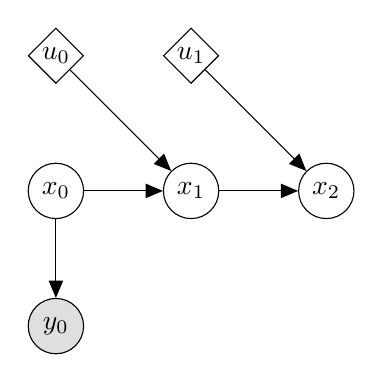
\begin{tikzpicture}

  % Define nodes
  \node[obs] (ya) {$y_{0}$};
  \node[latent, above=of ya] (xa) {$x_{0}$};
  \node[latent, right=of xa] (xb) {$x_1$};
  \node[latent, right=of xb]  (xc) {$x_{2}$};
  \node[det, above=of xa] (da) {$u_{0}$};
  \node[det, above=of xb] (db) {$u_{1}$};
  
  % Connect the nodes
  \edge {da} {xb};
  \edge {db} {xc};
  \edge {xa} {ya};
  \edge {xa} {xb};
  \edge {xb} {xc};
  
\end{tikzpicture}
\caption{Graphical model for state prediction.}
\label{fig_gm_mpc}
\end{figure}
Inspecting figure \ref{fig_gm_mpc} we note that the state prediction equations derived in section \ref{sec_lin_prediction} are applicable. Thus we can predict the state distributions given the future inputs $\mathbf{u}$.

Before we proceed we prove a very intuitive result in theorem \ref{thrm_optim_eq}. We will use this to link the predictive controller we derive here, using the results of sections \ref{sec_kalman_filter_deriv} and \ref{sec_lin_prediction}, to the LQR controller derived in section \ref{sec_lqr_lit}.
\begin{thrm}
\textbf{Optimisation Equivalence} Suppose we have two real valued convex objective functions $f(x_0,\mathbf{u})$ and $g(x_0, \mathbf{u})$ and we are required to minimise them with respect to $\mathbf{u}$ over the same space where they are both defined: $\mathbf{u}\in \mathcal{U}$ and $x_0 \in \mathcal{X}$. Furthermore, suppose there exists a real number $k$ such that $\forall \mathbf{u} \in \mathcal{U}$ we have that $g(x_0, \mathbf{u}) + k = f(x_0, \mathbf{u})$. Finally, assume the existence and uniqueness of the global minimiser for each problem. Then the global minimiser $\mathbf{u}^*$ of $g(x_0, \mathbf{u})$ is also the global minimiser of $f(x_0, \mathbf{u})$.
\label{thrm_optim_eq}
\end{thrm}
\begin{proof}
This proof only holds over functions which are at least twice differentiable. By assumption we know that $\mathbf{u}^*$ is the minimiser of $g(x_0, \mathbf{u})$ given $x_0$. By the necessary conditions for optimality \cite{forst} we know that $\nabla g(x_0, \mathbf{u}^*) = 0$ and that $\nabla ^2 g(x_0, \mathbf{u}^*)$ is positive semi-definite. Since $f$ and $g$ are both twice differentiable and  $g(x_0, \mathbf{u}^*) + k = f(x_0, \mathbf{u}^*)$ it must hold that $\nabla g(x_0, \mathbf{u}^*) = \nabla f(x_0, \mathbf{u}^*)$ and  $\nabla ^2 g(x_0, \mathbf{u}^*) = \nabla ^2 f(x_0, \mathbf{u}^*)$. Since $\nabla ^2 g(x_0, \mathbf{u}^*)$ is positive semi-definite it must be that $\nabla ^2 f(x_0, \mathbf{u}^*)$ is also positive semi-definite. Therefore $\mathbf{u}^*$ is necessarily a minimum of $f$. Since $f$ is convex the minimum must also be a global minimum.
\end{proof}
Now we are in a position to show the equivalence between the LQR control problem and the LQG control problem using the results of sections \ref{sec_kalman_filter_deriv} and \ref{sec_lin_prediction}. Theorem \ref{thrm_lqr_lqg_diff} shows how this is possible. It is quite reassuring to note that by starting within the framework of graphical models we arrive at the most important contribution of \cite{yan1} and \cite{yan2} in an intuitively simple manner.
\begin{thrm}
\textbf{LQR and LQG objective function difference} Consider the LQR, 
\begin{equation}
\begin{aligned}
&J_{LQR}(x_0, \mathbf{u}) = \frac{1}{2}\sum_{k=0}^{N-1} \left( x_k^TQx_k + u_k^TRu_k \right) + \frac{1}{2}x_N^TP_fx_N  \\
&\text{with } x_{t+1} = Ax_t +Bu_t,
\end{aligned}
\label{eq_lqr_obj_func}
\end{equation}
and LQG, 
\begin{equation}
\begin{aligned}
&J_{LQG}(x_0, \mathbf{u}) =  \mathbb{E}\left[ \frac{1}{2}\sum_{k=0}^{N-1} \left( x_k^TQx_k + u_k^TRu_k \right) + \frac{1}{2}x_N^TP_fx_N \right] \\
&\text{with } x_{t+1} = Ax_t +Bu_t + w_{t+1},
\end{aligned}
\label{eq_lqg_obj_func}
\end{equation}
objective functions. Suppose $x_0$ is the state estimate, assumed to be Gaussian, given the latest observation in the stochastic case. In the deterministic case we have that $x_0 = \mathbb{E}[x_0] = \mu_0$ because we exactly observe the state. Given any input sequence $\mathbf{u} \in \mathcal{U}$, where $\mathcal{U}$ is the shared admissible input space, we have that $J_{LQR}(x_0, \mathbf{u}) + \frac{1}{2}\sum_{k=0}^N \text{tr}(Q\Sigma_k) = J_{LQG}(x_0, \mathbf{u})$ where $ \Sigma_{t+1} = W+A\Sigma_t A^T$ and $\Sigma_0$ is the covariance matrix of the current state given by the observer.
\label{thrm_lqr_lqg_diff}
\end{thrm}
\begin{proof}
Expanding the LQG objective function (the expected value operator is linear) and noting that $\mathbf{u}$ is deterministic we have  
\begin{equation}
\begin{aligned}
J_{LQG}(x_0, \mathbf{u}) &= \frac{1}{2} \mathbb{E}\left[x_0^TQx_0\right] +\frac{1}{2} u_0^TRu_0 + \frac{1}{2} \mathbb{E}\left[x_1^TQx_1\right] + \frac{1}{2}u_1^TRu_1 + \hdots \\ &+ \frac{1}{2} \mathbb{E}\left[x_{N-1}^TQx_{N-1}\right]+ \frac{1}{2}u_{N-1}^TRu_{N-1} + \frac{1}{2} \mathbb{E}\left[x_N^TP_fx_N\right].
\end{aligned}
\label{eq_expanded_obj}
\end{equation}
We know that $x_0\sim \mathcal{N}(\mu_0, \Sigma_0)$ because the current state estimate was assumed to be Gaussian. This means that we can evaluate the first expected value in (\ref{eq_expanded_obj}) using theorem \ref{thrm_gaussian_identities} to write
\begin{equation}
\mathbb{E}\left[x_0^TQx_0\right] = \text{tr}(Q\Sigma_0) + \mu_0^TQ\mu_0.
\label{eq_exp1}
\end{equation} 
Now we turn our attention to the second expected value in (\ref{eq_expanded_obj}). First note that because we have $x_0$ and $\mathbf{u}$ we can use the result from section \ref{sec_lin_prediction} to predict the distribution of $x_1$. Therefore we know that $x_1 \sim \mathcal{N}(A\mu_0+Bu_0, W+A\Sigma_0 A^T)$. Now we let $\mu_1 = A\mu_0+Bu_0$ and $\Sigma_0 = W+A\Sigma_0 A^T$. Then by using theorem \ref{thrm_gaussian_identities} we have 
\begin{equation}
\mathbb{E}\left[x_1^TQx_1\right] = \text{tr}(Q\Sigma_1) + \mu_1^TQ\mu_1.
\label{eq_exp2}
\end{equation} 
Note that $\text{tr}(Q\Sigma_1)$ does not depend on $u_0$ but only on the initial state estimate $x_0$ which is independent of the future inputs $\mathbf{u}$. Notice that we can continue in this manner to simplify the LQG objective function to
\begin{equation}
\begin{aligned}
&J_{LQG}(x_0, \mathbf{u}) = \frac{1}{2}\sum_{k=0}^{N-1} \left( \mu_k^TQ\mu_k + u_k^TRu_k \right) + \frac{1}{2}\mu_N^TP_f\mu_N + \frac{1}{2}\sum_{k=0}^N \text{tr}(Q\Sigma_k) \\
&\text{with } \mu_{t+1} = A\mu_t +Bu_t \\
&\text{and } \Sigma_{t+1} = W+A\Sigma_t A^T.
\end{aligned}
\label{eq_simpl_obj_func}
\end{equation}
Now note that except for the last term $J_{LQG}(x_0, \mathbf{u})$ is exactly the same as $J_{LQR}(x_0, \mathbf{u})$. The conclusion follows because $\frac{1}{2}\sum_{k=0}^N \text{tr}(Q\Sigma_k)$ is independent of $\mathbf{u}$. 
\end{proof}
Finally we combine theorems \ref{thrm_optim_eq} and \ref{thrm_lqr_lqg_diff} to produce theorem \ref{thrm_lqg_sol}.
\begin{thrm}
\textbf{Solution of the finite horizon LQG control problem} We wish to solve the LQG control problem within the framework of graphical models. The full problem is 
\begin{equation}
\begin{aligned}
&\underset{\mathbf{u}}{\text{min }} V(x_0, \mathbf{u}) = \mathbb{E}\left[ \frac{1}{2}\sum_{k=0}^{N-1} \left( x_k^TQx_k + u_k^TRu_k \right) + \frac{1}{2}x_N^TP_fx_N \right] \\
& \text{subject to } x_{t+1}=Ax_t+Bu_t + w_t.
\end{aligned}
\label{eq_lqg_problem_full}
\end{equation}
We assume that $x_0$ is the current posterior state estimate, which is Gaussian, supplied by some observer. The solution of (\ref{eq_lqg_problem_full}) is equivalent to solving the LQR problem with initial state equal to the mean of the initial state estimate supplied by some observer.
\label{thrm_lqg_sol}
\end{thrm}
\begin{proof}
We assume that we have a Gaussian posterior state estimate for $x_0$. We use theorem \ref{thrm_lqr_lqg_diff} to prove that given $x_0$ and $\forall \mathbf{u} \in \mathcal{U}$ we have that $J_{LQR}(x_0, \mathbf{u}) + \frac{1}{2}\sum_{k=0}^N \text{tr}(Q\Sigma_k) = J_{LQG}(x_0, \mathbf{u})$ with $\frac{1}{2}\sum_{k=0}^N \text{tr}(Q\Sigma_k) \in \mathbb{R}$ a constant depending only on $x_0$. Thus we can use theorem \ref{thrm_optim_eq} to prove that we only need to solve for the optimal controller input $\mathbf{u}$ using the LQR objective function to solve (\ref{eq_lqg_problem_full}). 
\end{proof}
As we have mentioned before, the separation theorem (sometimes called certainty equivalence) implies that the solution of the LQG control problem is achieved by using the Kalman filter to optimally estimate the current state and then using that state estimate in the optimal LQR controller. It is reassuring that theorem \ref{thrm_lqg_sol} is confirmed by this result if we use the Kalman filter as the observer. The primary benefit of the graphical model approach is clear: we have solved the LQG problem without resorting to stochastic dynamical programming.

Under some circumstances it is also possible to extend the result of theorem \ref{thrm_lqg_sol} to the infinite horizon case as shown in theorem \ref{thrm_lqg_sol_inf}.
\begin{thrm}
\textbf{Solution of the infinite horizon LQG control problem} If the linear model of (\ref{eq_lin_system_control}) is stable then, using, with some minor adjustments, theorems \ref{thrm_optim_eq} and \ref{thrm_lqr_lqg_diff} it is possible to show that the infinite horizon LQG problem is solved in a similar manner: a Gaussian state estimate is used in conjunction with the infinite horizon LQR solution. This result can also be obtained by using the separation theorem. \label{thrm_lqg_sol_inf}
\end{thrm}
To clarify why it is important that the linear system (i.e. the matrix $A$) is stable, consider the quantity $\frac{1}{2}\sum_{k=0}^N \text{tr}(Q\Sigma_k)$. If it is unbounded the optimisation problem will be ill posed because the minimum will tend to some infinity. Inspecting $\Sigma_{t+1} = W+A\Sigma_t A^T$ we see that $||\Sigma_{\infty}||$ will be unbounded if $||A\Sigma_t A^T||$ becomes unbounded ($W$ is a constant) as $t \rightarrow \infty$. Note that $||\cdot||$ is some matrix norm. It can be shown that only if the eigenvalues of $A$ are less than unity i.e. the linear model is stable, then $||A\Sigma_{t+1}A^T|| \leq ||A\Sigma_{t}A^T||$ which implies that $\frac{1}{2}\sum_{k=0}^N \text{tr}(Q\Sigma_k)$ is bounded and the optimisation is reasonable.

\section{Constrained stochastic control}
\label{sec_lin_mpc_constained}
The goal of this section is to solve the stochastically constrained MPC optimisation problem
\begin{equation}
\begin{aligned}
&\underset{\mathbf{u}}{\text{min }} \mathbb{E}\left[ \frac{1}{2}\sum_{k=0}^{N-1} \left( x_k^TQx_k + u_k^TRu_k \right) + \frac{1}{2}x_N^TP_fx_N \right] \\
& \text{subject to } x_{t+1}=Ax_t+Bu_t + w_t \\
& \text{and } \mathbb{E}[d^Tx_t + e] \geq 0 ~\forall ~t=1,\hdots,N \\
& \text{and } \text{Pr}(d^Tx_t + e \geq 0) \geq p ~\forall ~t=1,\hdots,N.
\end{aligned}
\label{eq_mpc_constrained_linmod}
\end{equation}
We assume that the underlying system is linear and the probability distributions are Gaussian. From the results of chapter \ref{sec_inf_lin_mods} the probability distributions will be Gaussian if the system dynamics are linear. However, it is well known \cite{mac} that MPC is not in general a linear controller. From an analytical point of view this is problematic. We assume that the nonlinearity introduced by the MPC is negligible. We also restrict our analysis to affine constraints. Note that we only include one affine constraint in the succeeding examples however, the multiple constraint generalisation is addressed in the theory and are handled in exactly the same way as the examples using a single constraint. Furthermore, we assume that the current state estimate $x_0$ is supplied by some observer.

It might seem that the last constraint is a duplicate of the preceding one. Closer inspection reveals their different character. The first inequality constraint, which we will call the expected value constraint, requires that the predicted states satisfy the constraint ``on average" while the second inequality constraint, which we will call the chance constraint, requires that the predicted states satisfy the constraint with at least some probability $p$. 

For navigational convenience we supply a link to theorem \ref{thrm_mpc_stoch_to_det} - when the reader reaches that point the reason will become obvious.

Theorem \ref{thrm_affine_expected_const} succinctly shows that it is simple to convert the expected value constraint in (\ref{eq_mpc_constrained_linmod}) to a linear deterministic constraint.
\begin{thrm}
\textbf{Affine expected value constraints} Suppose we have a stochastic variable $x$ with a known Gaussian distribution and we also have $d \in \mathbb{R}^{n}$ and $e \in \mathbb{R}$. Then the stochastic constraint $\mathbb{E}[d^Tx + e] \geq 0$ simplifies to the deterministic constraint $d^T\mu + e \geq 0$ where $\mathbb{E}[x]= \mu$ is the mean of the stochastic variable. 

Furthermore, suppose we have the set of $n$ stochastic constraints $\mathbb{E}[Dx + e] \geq 0$. In this case $D \in \mathbb{R}^{n \times m}$ and $e \in \mathbb{R}^n$. Then $\mathbb{E}[Dx + e] \geq 0$ simplifies to $D\mu + e \geq 0$.  
\label{thrm_affine_expected_const}
\end{thrm}
\begin{proof}
We know that $x$ is a Gaussian stochastic variable. By theorem \ref{thrm_gaussian_identities} we know that $\mathbb{E}[d^Tx + e] =d^T\mu + e$ and $\mathbb{E}[Dx + e] = D\mu + e$. This immediately implies the result.
\end{proof}
It is interesting to pause here for a moment and consider theorem \ref{thrm_lqg_sol} and theorem \ref{thrm_affine_expected_const} applied to a problem of the form 
\begin{equation}
\begin{aligned}
&\underset{\mathbf{u}}{\text{min }} \mathbb{E}\left[ \frac{1}{2}\sum_{k=0}^{N-1} \left( x_k^TQx_k + u_k^TRu_k \right) + \frac{1}{2}x_N^TP_fx_N \right] \\
& \text{subject to } x_{t+1}=Ax_t+Bu_t + w_t \\
& \text{and } \mathbb{E}[d^Tx_t + e] \geq 0 ~\forall ~t=1,\hdots,N.
\end{aligned}
\label{eq_mpc_constrained_linmod_noprob}
\end{equation}
We assume that the current state estimate is available at each time step, that it is Gaussian and that $\mathbb{E}[x_0]=\mu_0$. It is clear that by applying theorems \ref{thrm_lqg_sol} and \ref{thrm_affine_expected_const} it is possible to rewrite (\ref{eq_mpc_constrained_linmod_noprob}) as
\begin{equation}
\begin{aligned}
&\underset{\mathbf{u}}{\text{min }} \frac{1}{2}\sum_{k=0}^{N-1} \left( \mu_k^TQ\mu_k + u_k^TRu_k \right) + \frac{1}{2}\mu_N^TP_f\mu_N + \frac{1}{2}\sum_{k=0}^N \text{tr}(Q\Sigma_k) \\
& \text{subject to } \mu_{t+1}=A\mu_t + Bu_t \\
& \text{and } d^T\mu_t + e \geq 0 ~\forall ~t=1,\hdots,N.
\end{aligned}
\label{eq_mpc_constrained_linmod_deter_noprob}
\end{equation}
This implies that the standard deterministic MPC problem (\ref{eq_mpc_constrained_linmod_deter_noprob}) is equivalent to the stochastic MPC problem with affine expected value constraints (\ref{eq_mpc_constrained_linmod_noprob}) under the assumptions of linearity and normality. This suggests that if chance constraints are not required the standard deterministic MPC will be sufficient for the control of stochastic processes. The generalisation of (\ref{eq_mpc_constrained_linmod_noprob}) to multiple expected value constraints is straightforward due to the second part of theorem \ref{thrm_affine_expected_const}. 

Theorem \ref{thrm_mahala_dist} is a necessary step before we can convert the chance constraint of (\ref{eq_mpc_constrained_linmod}) into a nonlinear deterministic constraint.
\begin{thrm}
\textbf{Shortest squared Mahalanobis distance between a hyperplane and a point} Suppose we are given a symmetric positive semi-definite matrix $S$ and a point $y$. The shortest squared Mahalanobis distance between $y$ and the hyperplane $b^Tx+c=0$ is given by $\frac{(b^Ty+c)^2}{b^TSb}$.
\label{thrm_mahala_dist}
\end{thrm}
\begin{proof}
It is natural to formulate theorem \ref{thrm_mahala_dist} as an optimisation problem
\begin{equation}
\begin{aligned}
&\underset{x}{\text{min }} (x-y)^TS^{-1}(x-y)\\
& \text{subject to } b^Tx+c = 0.
\end{aligned}
\label{eq_mahala_optim}
\end{equation}
Note that $S$ and therefore also $S^{-1}$ is symmetric. Using conventional calculus we have $\nabla f(x) = (S^{-1} + {S^{-1}}^T)x - 2S^{-1}y = 2S^{-1}x - 2S^{-1}y$ and $\nabla g(x) = b^T$. Using the method of Lagrangian multipliers \cite{forst} we have the system of equations
\begin{equation}
\begin{aligned}
2S^{-1}x - 2S^{-1}y + \lambda b = 0 \\
b^Tx+c = 0.
\end{aligned}
\label{eq_lagrange_eqs}
\end{equation}
This can be rewritten in block matrix form 
\begin{equation}
\begin{pmatrix}
2S^{-1} & b \\ b^T & 0
\end{pmatrix} \begin{pmatrix}
x \\ \lambda
\end{pmatrix} = \begin{pmatrix}
2S^{-1}y \\ -c
\end{pmatrix}.
\label{eq_lagrange_block}
\end{equation}
The special structure of the left hand side matrix in (\ref{eq_lagrange_block}) allows us to analytically compute the inverse (see theorem \ref{thrm_block_inv} in section \ref{sec_block})
\begin{equation}
\begin{pmatrix}
2S^{-1} & b \\ b^T & 0
\end{pmatrix}^{-1} = \begin{pmatrix}
\frac{1}{2}S(I-\frac{bb^TS}{b^TSb}) & \frac{Sb}{b^TSb} \\ \frac{b^TS}{b^TSb} & -\frac{2}{b^TSb}
\end{pmatrix}.
\label{eq_lagrance_block_inverse}
\end{equation}
To find the arguments which satisfy (\ref{eq_lagrange_eqs}) we solve
\begin{equation}
\begin{pmatrix}
\frac{1}{2}S(I-\frac{bb^TS}{b^TSb}) & \frac{Sb}{b^TSb} \\ \frac{b^TS}{b^TSb} & -\frac{2}{b^TSb} \end{pmatrix} \begin{pmatrix}
2S^{-1}y \\ -c
\end{pmatrix} = \begin{pmatrix}
S(I-\frac{bb^TS}{b^TSb})S^{-1}y - c\frac{Sb}{b^TSb} \\
2(\frac{b^TS}{b^TSb} + \frac{c}{b^TSb})
\end{pmatrix}
\label{eq_lagrange_args}
\end{equation}
which is equivalent to solving the system of linear equations in (\ref{eq_lagrange_block}). Therefore, the arguments which minimise (\ref{eq_mahala_optim}) are $x^* = S(I-\frac{bb^TS}{b^TSb})S^{-1}y - c\frac{Sb}{b^TSb}$. Substituting this into the objective function we have
\begin{equation}
\begin{aligned}
&\left(x^*-y\right)^TS^{-1}\left(x^*-y\right) \\ 
&= \left(S\left(I-\frac{bb^TS}{b^TSb}\right)S^{-1}y - c\frac{Sb}{b^TSb}-y\right)^TS^{-1}\left( S \left(I-\frac{bb^TS}{b^TSb}\right)S^{-1}y - c \frac{Sb}{b^TSb}-y\right) \\ 
&= \left(\frac{Sbb^Ty}{b^TSb} + c\frac{Sb}{b^TSb}\right)^TS^{-1}\left(\frac{Sbb^Ty}{b^TSb}+ c\frac{Sb}{b^TSb}\right) \\
&= \frac{(Sb)^T}{b^TSb}\left( b^Ty+c \right)^TS^{-1}\frac{Sb}{b^TSb}\left(b^Ty+c\right) \\
&= \frac{b^TS}{b^TSb}\left(b^Ty+c\right)^T\frac{b}{b^TSb}\left(b^Ty+c\right) \\
&= \left(b^Ty+c\right)^T\frac{b^TSb}{(b^TSb)^2}\left(b^Ty+c\right) \\
&= \frac{(b^Ty+c)^T(b^Ty+c)}{b^TSb} \\
&= \frac{(b^Ty+c)^2}{b^TSb}.
\end{aligned}
\label{eq_lagrange_min}
\end{equation}
We can conclude that the shortest squared Mahalanobis distance between a point $y$ and the constraint of (\ref{eq_mahala_optim}) is $\frac{(b^Ty+c)^2}{b^TSb}$.
\end{proof}
In theorem \ref{thrm_chance_cons} we apply theorem \ref{thrm_mahala_dist} to convert the chance constraints into nonlinear deterministic constraints.
\begin{thrm}
\textbf{Gaussian affine chance constraints} Suppose the underlying distribution of a random variable $x$ is Gaussian with sufficient statistics ($\mu, \Sigma$) and we have that $d \in \mathbb{R}^{n}$ and $e \in \mathbb{R}$. Also, suppose that $d^T\mu+e>0$ is ensured.

Then the chance constraint $\text{Pr}(d^Tx + e \geq 0) \geq p$ can be rewritten as the deterministic constraint $\frac{(d^T\mu+e)^2}{d^T \Sigma d} \geq k^2$ where $k^2$ is the (constant) critical value of the inverse cumulative Chi Squared distribution with the degrees of freedom equal to the dimensionality of $x$ such that $\text{Pr}(\mathcal{X} \leq k^2) = p$ with $\mathcal{X}$ a Chi Squared random variable. Note that $p > 0.5$ due to the fact that $d^T\mu+e>0$ is ensured.

Furthermore, suppose $D \in \mathbb{R}^{n\times m}$, $e \in \mathbb{R}^n$ and $D\mu + e >0$ which, again, implies that $p > 0.5$. Then joint chance constraint $\text{Pr}(Dx + e \geq 0) \geq p$ can be written: for all $i=1,\hdots,n$ we require $\frac{(d^T_i\mu+e_i)^2}{d_i^T \Sigma d_i} \geq k^2$. Note $d_i$ is each row in $D$ and $e_i$ each corresponding element in $e$.
\label{thrm_chance_cons}
\end{thrm}
\begin{proof}
Intuitively theorem \ref{thrm_chance_cons} posits that if the shortest squared Mahalanobis distance is further away than some threshold $k^2$ the chance constraint $\text{Pr}(d^Tx + e \geq 0) \geq p$ will be satisfied. Figure \ref{fig_mahala_ellipse} depicts the idea that the minimum squared Mahalanobis distance must be greater than $k^2$ i.e. $\epsilon > 0$. The use of the Mahalanobis distance is important because it takes into account the uncertainty associated with each component of the random variable $x$.  
\begin{figure}[H] 
\centering
\includegraphics[scale=0.7]{ellipse2.pdf}
\caption{The ellipse centred around $\mu_1$ intersects the constraint while the ellipse centred around $\mu_2$ is wholly above (satisfies) the constraint. The shortest Mahalanobis distance will not necessarily be perpendicular to the constraint.}
\label{fig_mahala_ellipse}
\end{figure}
Since $x$ is a Gaussian stochastic variable we have that $\mathbb{E}[x] =\mu$ and $\text{var}[x]=\Sigma$. Let $\Omega = \{x \in \mathbb{R}^n~|~(x-\mu)^T\Sigma^{-1}(x-\mu) \leq k^2\}$ and $k^2$ be the critical value such that for the Chi Squared distribution with degrees of freedom equal to the dimension of $x$ we have that $\text{Pr}(\mathcal{X} \leq k^2) = p$. Then it is well known \cite{mahala2} that $\int_{\Omega}p(x|\mu, \Sigma)dx = p$ where $p(\cdot|\mu, \Sigma)$ is the multivariate Gaussian probability distribution function of $x$. If the shortest squared Mahalanobis distance from the mean of $x$ is further away from the affine constraint $d^Tz+e=0$ than $k^2$ it implies that the curve of the function $h(z) = (z-\mu)^T\Sigma^{-1}(z-\mu) = k^2$ does not intersect with the constraint - a positive $\epsilon$ in the context of figure \ref{fig_mahala_ellipse}. Therefore $\Omega$ is wholly contained within the feasible region because $d^T\mu+e> 0 $. This implies, with at least a probability of $p$, that the chance constraint will not be violated because the ``confidence ellipse" is contained in the feasible region. Therefore, by applying theorem \ref{thrm_mahala_dist} to find the shortest squared Mahalanobis distance between $\mu$ and the constraint we have that $\frac{(d^T\mu+e)^2}{d^T \Sigma d} \geq k^2 \implies \text{Pr}(d^Tx + e \geq 0) \geq p$.

The generalisation to more than one constraint, which should be jointly satisfied, is shown in figure \ref{fig_mahala_ellipse_joint}. It is required that the ellipse, up to confidence level $p$, is wholly contained in the feasible region $Dx +e >0$. If this requirement is satisfied we will satisfy the joint chance constraint by the same reasoning as before.  
\begin{figure}[H] 
\centering
\includegraphics[scale=0.8]{multiple.pdf}
\caption{Illustration of the fact that theorem \ref{thrm_chance_cons} holds jointly for multiple constraints. The ellipse centred around $\mu$ must lie wholly within the feasible region. This is guaranteed if the Mahalanobis constraint is satisfied.}
\label{fig_mahala_ellipse_joint}
\end{figure}
By ensuring that $D\mu + e > 0$ and that the shortest squared Mahalanobis distance between $\mu$ and the constraints is bigger than $k^2$ this is guaranteed. This implies that if for all $i=1,\hdots,n$ $\frac{(d^T_i\mu+e_i)^2}{d_i^T \Sigma d_i} \geq k^2$ then $\text{Pr}(Dx + e \geq 0) \geq p$ will be satisfied.
\end{proof}
In theorem \ref{thrm_chance_cons} it is important that $\mu$ lie within the feasible region. If that is not required then it is possible for the ellipse to be wholly outside the feasible region while still satisfying the requirement that the shortest squared Mahalanobis distance between $\mu$ and the constraints is at least $k^2$. Clearly the chance constraint will then not be satisfied. 

It is interesting to note the striking similarity between the work in \cite{vanhessem1} and \cite{vanhessem2} and theorem~\ref{thrm_chance_cons} given that we started analysing the problem within the framework of graphical models. The additional benefit of theorem \ref{thrm_chance_cons} is that it formulates the chance constraint as a function of the statistical Mahalanobis distance measure. This is useful because it lends a statistical interpretation to theorem \ref{thrm_chance_cons} even if the underlying distribution is non-Gaussian.

In theorem \ref{thrm_mpc_stoch_to_det} we combine and elaborate on the work of \cite{yan1}, \cite{vanhessem1} to yield a QP MPC which exactly satisfies the stochastic MPC in (\ref{eq_mpc_constrained_linmod}) given the assumptions of linearity and normality. Note that the dimensionality of the problem is arbitrary.
\begin{thrm}
\textbf{Conversion of the stochastic MPC formulation to the standard deterministic QP MPC formulation} Under the assumptions of linearity and Gaussian distributions we can reformulate the stochastic MPC problem shown in (\ref{eq_mpc_constrained_linmod}) as a standard deterministic quadratic programming MPC problem
\begin{equation}
\begin{aligned}
&\underset{\mathbf{u}}{\text{min }} \frac{1}{2}\sum_{k=0}^{N-1} \left( \mu_k^TQ\mu_k + u_k^TRu_k \right) + \frac{1}{2}\mu_N^TP_f\mu_N + \frac{1}{2}\sum_{k=0}^N \text{tr}(Q\Sigma_k) \\
& \text{subject to } \mu_{t+1}=A\mu_t + Bu_t \\
& \text{and } \Sigma_{t+1} = W+A\Sigma_t A^T \\
& \text{and } d^T\mu_t + e \geq k\sqrt{d^T \Sigma_t d} ~\forall ~t=1,\hdots,N.
\end{aligned}
\label{eq_mpc_constrained_linmod_deter}
\end{equation}
\label{thrm_mpc_stoch_to_det}
Other deterministic constraints, e.g. on the input, can be added as usual. Note that we have assumed that the initial state estimate $x_0$ is available in the form of its mean, $\mu_0$,  and covariance, $\Sigma_0$. It is straightforward to include more chance constraints. Since each chance constraint is reduced to an inequality constraint which measures the Mahalanobis distance between the predicted distributions, the resultant feasible points will jointly satisfy all chance constraints.  
\end{thrm}
\begin{proof}
Let the admissible set of controller inputs $\mathcal{U}$ be the same for both the stochastic MPC and the deterministic MPC formulations. Furthermore, let the current state estimate $x_0$ be given. Then by theorem~\ref{thrm_lqr_lqg_diff} the objective function and equality constraints follow. By theorem~\ref{thrm_affine_expected_const} the expected value inequality constraint in (\ref{eq_mpc_constrained_linmod}) can be reformulated to require that $d^T\mu_t + e \geq 0$ for each $t=1, 2,\hdots, N$. The chance constraint in (\ref{eq_mpc_constrained_linmod})  can be reformulated by using theorem \ref{thrm_chance_cons}:
\begin{equation}
\begin{aligned}
\frac{(d^T\mu_t+e)^2}{d^T \Sigma_t d} \geq k^2 &\implies (d^T\mu_t+e)^2 \geq k^2 {d^T \Sigma_t d} \\
&\implies d^T\mu_t+e \geq k \sqrt{d^T \Sigma_t d}~\forall~t=1, 2,\hdots, N.
\end{aligned}
\label{eq_chance_to_lin}
\end{equation}
The first line of (\ref{eq_chance_to_lin}) follows because $\Sigma_t$ is positive semi-definite for all $t=1, 2,\hdots, N$ and $d \neq 0$ (otherwise it would not be a constraint), therefore it can be multiplied over the inequality sign like a positive number. By theorem \ref{thrm_lqg_sol} we have that $\Sigma_{t+1} = W + A\Sigma_tA^T$, therefore the predicted covariance matrices used in (\ref{eq_chance_to_lin}) are well defined. The second line follows because of the first inequality constraint: we know that $d^T\mu_t+e \geq 0 ~\forall~t=1,2,\hdots, N$ and therefore we can square root both sides of the inequality constraint. Thus we have the two inequality constraints $d^T\mu_t+e \geq 0$ and $d^T\mu_t+e \geq k \sqrt{d^T \Sigma_t d}$ for each $t=1,2,\hdots,N$. Since $k > 0$ (otherwise we do not have a meaningful chance constraint) we can condense the two inequality constraints into a single constraint: $d^T\mu_t+e \geq k \sqrt{d^T \Sigma_t d} > 0$ for each $t=1,2,\hdots,N$ from which the conclusion follows.  
\end{proof}
The beauty of theorem \ref{thrm_mpc_stoch_to_det} is that no new theory is necessary to analyse the stability and convergence results of the new MPC. This is highly desirable because it allows one to merely ``add" the inequality constraint in (\ref{eq_mpc_constrained_linmod_deter}) to your existing MPC formulation. Most practical MPCs will have some form of state estimation and thus no new parameters are introduced either. Since the problem is in standard QP form it is straightforward to implement and, even more importantly, it is computationally fast because the problem is trivially convex.

In the work by \cite{yan1} and \cite{yan2}, which primarily dealt with univariate problems, it was found that feasibility problems might arise if one uses the predicted covariance estimates in the controller. If the system is unstable the uncertainty in the estimates can grow with time as discussed in theorem \ref{thrm_lqg_sol_inf}. This can cause the ellipses used in theorem \ref{thrm_chance_cons} to become too large to fit inside the feasible region. The approach adopted by \cite{yan1} and \cite{yan2} is to only use the one step ahead predicted covariance ($\Sigma_1$) over the entire prediction horizon. This does not ensure feasibility but restricts the growth associated with infeasibility. The drawback of this approach is that it might cause constraint violation because the controller will be more aggressive.  

\section{Reference tracking}
So far we have only dealt with controllers which drive the system to the origin. The more general situation we are interested in is arbitrary reference point tracking. Fortunately, section~\ref{sec_lit_ref_track} applies without modification because the stochastic MPC problem was reduced to the \textit{standard} deterministic MPC problem. 

\section{Linear system}
\label{sec_lin_sys_cont}
In this section we consider the problem of controlling a linear system using the stochastic MPC formulation of theorem \ref{thrm_mpc_stoch_to_det}. More precisely, we assume the linear model linearised about the unsteady operating point of our CSTR example from chapter \ref{sec_cstr} accurately represents the underlying system. For the purposes of illustration we will only use the (somewhat unrealistic) system where both states are measured. However, there is no theoretical reason why we cannot use the system where only temperature is measured. The drawback of using the latter system is that inference, as discussed previously, will be worse. The control goal is to steer the concentration, in the sense of definition \ref{def_stoch_ref_track_goal}, to the unsteady operating point ($C_A = 0.49$ kmol.m$^{-3}$) about which the system was linearised. See chapter \ref{sec_cstr} for more details.

We repeat the relevant system dynamics  
\begin{equation}
\begin{aligned}
&A = \begin{pmatrix}
0.9959 & -6.0308\times 10^{-5} \\
0.4186 & 1.0100
\end{pmatrix}
~~B = \begin{pmatrix}
0 \\ 8.4102\times 10^{-5}
\end{pmatrix} ~~
C = \begin{pmatrix}
1 & 0 \\ 0 & 1
\end{pmatrix} \\
&W = \begin{pmatrix}
1\times 10^{-6} & 0 \\ 0 & 0.1
\end{pmatrix} ~~
V = \begin{pmatrix}
1\times 10^{-3} & 0 \\ 0 & 10
\end{pmatrix}
\end{aligned}
\label{eq_linmod_params}
\end{equation}
using a time step $h=0.1$. The tuning parameters used in this and all subsequent chapters are 
\begin{equation}
\begin{aligned}
Q = P_f = \begin{pmatrix}
1\times 10^{4} & 0 \\ 0 & 0
\end{pmatrix} 
~~R = \begin{pmatrix}
1\times 10^{-6}
\end{pmatrix}
\end{aligned}
\label{eq_mpc_tuning}
\end{equation}
Note that the magnitude difference between the components of $Q$, $P_f$ and $R$ is necessary because the units of concentration and heat input are not scaled. We assume that a Kalman filter supplies the current posterior state estimate $x_0$ at each time step. Additionally, we assume a zero order hold of 1 min between controller inputs.

It is useful to introduce the measures we will use to quantify the effectiveness of the control techniques used in this and the following chapters. We define the average energy input by $\frac{1}{N}\sum^N_{t=0}|u_t-u_s|$ and the average concentration error by $\frac{1}{N}\sum^N_{t=0}|\frac{{C_A}_t-y_{sp}}{y_{sp}}|$. Additionally, to confirm that the results hold true over multiple simulations we will, at the end of sections~\ref{sec_lin_sys_cont} and \ref{sec_nonlinear_control}, include a Monte-Carlo simulation. The metrics we use for the Monte Carlo simulations will be the time each simulation spent in violation of the constraints and the total state space area (measured within the context of the Mahalanobis distance) in violation of the constraint.  

First we illustrate the approach of using only the result of theorem \ref{thrm_lqg_sol} i.e. we apply the LQG regulator to the system. Based on our previous results we know that given the Kalman filter's current posterior state estimate mean, $\mu_0$, we only need to solve the LQR problem, 
\begin{equation}
\begin{aligned}
&\underset{\mathbf{u}}{\text{min }} \frac{1}{2}\sum_{k=0}^{N-1} \left( \mu_k^TQ\mu_k + u_k^TRu_k \right) + \frac{1}{2}\mu_N^TP_f\mu_N \\
& \text{subject to } \mu_{t+1}=A\mu_t + Bu_t,
\end{aligned}
\label{eq_lqg_linmod}
\end{equation}
to solve the LQG problem. The prediction horizon $N$ is set at 150 time steps i.e. 15 minutes into the future. Figure \ref{fig_lin_mod_lqg} shows that the system does indeed converge, noisily, to the set point. This is not surprising because we have effectively just implemented the very well studied LQG controller. The primary drawback of this method is that there is no easy way to constrain the system. From a practical perspective this can be problematic. 
\begin{figure}[H] 
\centering
\includegraphics[width=\textwidth]{lin_mod_lqg.pdf}
\caption{Unconstrained LQG regulator tracking with initial condition $(0.55, 450)$ and measuring both states.}
\label{fig_lin_mod_lqg}
\end{figure}
The average heat energy usage (controller input) over the simulation run is 24.99 kW. The average set point error is 2.29\% over the same 80 min time period.
 
Next we illustrate the approach of using conventional deterministic MPC to control the stochastic system. The MPC problem is
\begin{equation}
\begin{aligned}
&\underset{\mathbf{u}}{\text{min }} \frac{1}{2}\sum_{k=0}^{N-1} \left( \mu_k^TQ\mu_k + u_k^TRu_k \right) + \frac{1}{2}\mu_N^TP_f\mu_N \\
& \text{subject to } \mu_{t+1}=A\mu_t + Bu_t \\
&\text{and } \begin{pmatrix}
10 \\ 1
\end{pmatrix}^T \mu_t + 412 \geq 0 ~\forall ~t=1,\hdots,N\\
& \text{and } |u_t| \leq 165 ~\forall ~t=0,\hdots,N-1.
\end{aligned}
\label{eq_mpc_constrained_det1}
\end{equation}
Using MPC allows us to easily add state and input constraints; this is a significant improvement over conventional LQG as discussed previously. We only use a single state constraint in this dissertation but the extension to multiple constraints is straightforward. The prediction and control horizon are equal to each other and set at 150 time steps i.e. 15 minutes into the future. We additionally constrain the magnitude of the inputs.

Due to assumption of normality and linearity and by theorem \ref{thrm_lqg_sol} and \ref{thrm_affine_expected_const} we can also interpret the deterministic MPC as a stochastic MPC with an affine expected value constraint. Therefore the controller in (\ref{eq_mpc_constrained_det1}) is not inappropriate for the control of the stochastic CSTR process under consideration.

In figure \ref{fig_lin_mod_kf_mean_track} we see the reference tracking and controller input for the deterministic MPC. The average heat energy input and set point error over the simulation run is 28.22 kW and 2.43\% respectively. Interestingly the average error is not much different but the controller requires more energy to track the set point. This is reasonable because the additional constraints make problem (\ref{eq_mpc_constrained_det1}) a harder problem than (\ref{eq_lqg_linmod}).
\begin{figure}[H] 
\centering
\includegraphics[width=\textwidth]{lin_mod_kf_mean_track.pdf}
\caption{Deterministic constrained MPC tracking with initial condition $(0.55, 450)$ and measuring both states.}
\label{fig_lin_mod_kf_mean_track}
\end{figure}
Like the LQG controller, it is clear that we have noisy convergence to the set point. As mentioned previously we will never be able to achieve zero set point offset because of the noise term in the system dynamics (\ref{eq_lin_system}). Note that we have constrained the maximum magnitude of the inputs such that $|u_t| \leq 165$ kW. In the unconstrained case the controller required a maximum absolute input magnitude of over $200$ kW; the ability to naturally constrain the inputs can be practically very useful. The benefit of MPC is apparent here.

In figure \ref{fig_lin_mod_kf_mean_ss} we see the corresponding state space trajectory of the system together with the state constraint.
\begin{figure}[H]
\centering
\includegraphics[width=\textwidth]{lin_mod_kf_mean_ss.pdf}
\caption{Deterministic MPC state space trajectory with initial condition $(0.55, 450)$ and measuring both states. The red line is the constraint.}
\label{fig_lin_mod_kf_mean_ss}
\end{figure}
While the predicted mean state estimates do not violate the constraint (due to the optimisation constraints) the actual underlying system does.  This is clearly seen if one inspects the confidence region around the lower state estimates in figure \ref{fig_lin_mod_kf_mean_ss}. The confidence region is deeply violated by the constraint which implies that it is likely that the underlying system might. This is clearly a problem from a control point of view; the deterministic MPC cannot ensure that the constraint is satisfied.

We remedy this situation by introducing the chance constrained MPC as discussed in theorem~\ref{thrm_mpc_stoch_to_det}
\begin{equation}
\begin{aligned}
&\underset{\mathbf{u}}{\text{min }} \frac{1}{2}\sum_{k=0}^{N-1} \left( \mu_k^TQ\mu_k + u_k^TRu_k \right) + \frac{1}{2}\mu_N^TP_f\mu_N + \frac{1}{2}\sum_{k=0}^N \text{tr}(Q\Sigma_k) \\
& \text{subject to } \mu_{t+1}=A\mu_t + Bu_t \\
& \text{and } \Sigma_{t+1} = W+A\Sigma_t A^T \\
& \text{and } d^T\mu_t + e \geq k\sqrt{d^T \Sigma_t d} ~\forall ~t=1,\hdots,N\\
& \text{and } |u_t| \leq 165 ~\forall ~t=0,\hdots,N-1.
\end{aligned}
\label{eq_mpc_linmod_kf_cons}
\end{equation}
Note that $d^T = (10, 1)$ and $e=412$ as before. By consulting a Chi Squared distribution table we set $k^2 = 4.6052$ which corresponds to the chance constraint $\text{Pr}(d^Tx_t + e \geq 0) \geq 90\% ~\forall ~t=1,\hdots,N$. Note that problem (\ref{eq_mpc_linmod_kf_cons}) is harder than (\ref{eq_mpc_constrained_det1}) due to the added constraint and thus we expect that the system will require greater controller input to satisfy the constraint. 

In figure \ref{fig_lin_mod_kf_var90_track} we see that the stochastic MPC is able to track the set point in a similar manner as the LQG controller and deterministic MPC. The total average heat input and set point error over the simulation run is  38.58 kW and 2.58\% respectively. This problem is harder than the preceding one due to the additional constraint and thus more energy is required. 
\begin{figure}[H] 
\centering
\includegraphics[width=\textwidth]{lin_mod_kf_var90_track.pdf}
\caption{Chance constrained MPC tracking with initial condition $(0.55, 450)$ and measuring both states. A Kalman filter is used for inference and the chance constraint is set at 90\%.}
\label{fig_lin_mod_kf_var90_track}
\end{figure}
However, the benefit of adding the chance constraint is apparent in figure \ref{fig_lin_mod_kf_var90_ss}. It is clear that the constraint on the underlying state is not violated.
\begin{figure}[H] 
\centering
\includegraphics[width=\textwidth]{lin_mod_kf_var90_ss.pdf}
\caption{Chance constrained MPC state space trajectory with initial condition $(0.55, 450)$ and measuring both states. A Kalman filter is used for inference and the chance constraint is set at 90\%.}
\label{fig_lin_mod_kf_var90_ss}
\end{figure}
Since the chance constraint is only enforced with probability 90\% it is possible that the underlying system can come ``close" to the constraint. This then has the consequence that the posterior confidence region marginally violates (spills over) the constraint as seen in the lower regions of figure \ref{fig_lin_mod_kf_var90_ss}.
 
It is interesting to investigate what effect increasing the probability that the chance constraint is satisfied will have on the system. To this end we modify the chance constraint of (\ref{eq_mpc_linmod_kf_cons}) such that $k^2 = 9.21$ which corresponds to the chance constraint $\text{Pr}(d^Tx_t + e \geq 0) \geq 99\% ~\forall ~t=1,\hdots,N$. We expect that the underlying system will be moved further away from constraint due to this added level of conservativeness.

In figure \ref{fig_lin_mod_kf_var99_track} we see that the stochastic MPC still tracks the set point and figure \ref{fig_lin_mod_kf_var99_ss} shows that the expected behaviour is realised. 
\begin{figure}[H] 
\centering
\includegraphics[width=\textwidth]{lin_mod_kf_var99_track.pdf}
\caption{Chance constrained MPC tracking with initial condition $(0.55, 450)$ and measuring both states. A Kalman filter is used for inference and the chance constraint is set at 99\%.}
\label{fig_lin_mod_kf_var99_track}
\end{figure}
The average heat input and average set point error is 3.49\% and  58.39 kW. The added conservativeness of the MPC prevents it from attempting to get to the set point as fast as the previous stochastic MPC; consequently there is no set point overshoot in figure \ref{fig_lin_mod_kf_var99_track}. This causes the higher average error but the constraints are satisfied more robustly. As before, the control problem is harder and thus requires more energy.

In figure \ref{fig_lin_mod_kf_var99_ss} we see the 90\% confidence region is above the constraint. Since the probability that the predicted states are close to the constraint is much lower than before we see that the confidence region satisfies the constraint more robustly.
\begin{figure}[H] 
\centering
\includegraphics[width=\textwidth]{lin_mod_kf_var99_ss.pdf}
\caption{Chance constrained MPC state space trajectory with initial condition $(0.55, 450)$ and measuring both states. A Kalman filter is used for inference and the chance constraint is set at 99\%.}
\label{fig_lin_mod_kf_var99_ss}
\end{figure}
It would also be correct to infer that $k$ can be used as an empirical measure of the inherent stochastic conservativeness of the resulting controller. That is, lower values of $k$ indicate a more aggressive controller which may violate the chance constraints and higher values of $k$ indicate a more conservative controller. This can be useful for systems where the normal assumption is not valid but one would still like to enforce chance constraints in some empirical sense. 

We have made the strong assumption that the system dynamics remain linear and Gaussian even under the MPC control law which is not necessarily linear \cite{mac}. Clearly if the system is far from Gaussian the Gaussian approach to simplifying the chance constraint will not be valid. Fortunately this is relatively simple to check and serves as a good way of measuring controller health. That is, the more Gaussian the filtered distributions are, the better the linear stochastic controller will work. 

Kullback-Leibler Divergence was introduced in theorem \ref{thrm_kl_sample} to estimate the degree to which samples match a given distribution. From chapter \ref{sec_inf_nonlin_mods} we know that given enough particles a particle filter can accurately represent any distribution. Thus we temporarily replace the Kalman filter with a particle filter and use theorem \ref{thrm_kl_sample} to estimate the degree of normality of the posterior state distributions.

Figure \ref{fig_lin_mod_kl} shows the degree to which the underlying distribution is Gaussian. Since we cannot use an infinite number of particles we compare the sampled Gaussian distribution approximation to a baseline.   
\begin{figure}[H] 
\centering
\includegraphics[width=\textwidth]{lin_mod_kl.pdf}
\caption{Kullback-Leibler Divergence between the assumed Gaussian distribution and different sampled distributions using 5000 particles. The underlying model is linear.}
\label{fig_lin_mod_kl}
\end{figure}
The approximation curve in figure \ref{fig_lin_mod_kl} shows how much the samples diverge from the Gaussian distribution approximated using the samples. The baseline curve shows how much the Gaussian distribution diverges from samples of the same distribution. The uniform curve shows how much a Gaussian approximation of a Uniform distribution drawn in the interval $(\mu_i-2\sigma_{ii}, \mu_i+2\sigma_{ii})$ (for each $i$ in the dimension of the underlying distribution) diverges; this serves to illustrate the divergence one would expect if attempting to model a distribution which is decidedly not normal. One would expect the baseline curve to tend to zero as the number of particles tends to infinity. Sampling error causes divergence from zero for the baseline curve. Thus we can use the baseline and uniform curves as a crude measure of normality.

In figure \ref{fig_lin_mod_kl} we see that the approximation is relatively close to the baseline. Additionally it is far removed from the uniform curve. The average divergence for the baseline, approximation and uniform curve (in nats) is: $0.035$, $0.069$ and $0.322$ respectively. This implies that even though we are using a nonlinear control technique the posterior state distributions are still approximately Gaussian. 

In figure \ref{fig_lin_mod_kf_mc} we investigate the effect $k^2$ has on the chance constraint. We expect that by increasing $k^2$ the system becomes more conservative and less likely to violate the constraint. Under the assumptions of linearity and normality we are assured of this behaviour due to theorem \ref{thrm_mpc_stoch_to_det}. However, as figure \ref{fig_lin_mod_kl} indicates our assumptions do not  strictly hold. In figures \ref{fig_lin_mod_kf_var90_ss} and \ref{fig_lin_mod_kf_var99_ss} we reached the conclusion that the chance constraint was effective by only considering a single simulation. In figure \ref{fig_lin_mod_kf_mc} we show the compilation of over 2000 runs to illustrate the veracity of the claim that the chance constraints are effective.
\begin{figure}[H] 
\centering
\includegraphics[width=\textwidth]{lin_mod_kf_mc.pdf}
\caption{Monte-Carlo simulation to investigate the effect increasing $k^2$ has on the constraint violation characteristics of the MPC controllers. Each region indicates where 90\% of the simulations scored. The mean is indicated by a solid point.}
\label{fig_lin_mod_kf_mc}
\end{figure}
The Mahalanobis area dimension indicates the degree to which the constraint was violated: larger numbers imply the constraint was deeply violated in state space. The time in violation dimension indicates the length of time the system violated the constraint. It is clear that the chance constraints dramatically reduce the violation characteristics of the system. 

Interestingly, there seems to be diminishing returns on increasing $k^2$ beyond the 99\% chance interval. Feasibility issues plague the system under the more conservative chance constraint levels. Intuitively the predicted ellipses become too big to fit inside the feasible region - especially when projected forward in time. Given that the controller input - the only way to move them inside the feasible region - is constrained the system reaches a performance deadlock. In the work by \cite{yan1} they also noted this problem and solved it by not letting the confidence ellipses grow as they were projected into the future (see the discussion after theorem \ref{thrm_lqg_sol_inf} and in section \ref{sec_switch_mpc_lit}). For this system the issue is not severe enough to warrant further concern.   

Finally, we illustrate that the MPC controllers we developed, using the linear underlying model, actually drive the system to the set point for many runs - not just the single realisation we considered so far. In figure \ref{fig_lin_mod_kf_mc2} a Monte Carlo simulation was conducted using 50 runs per controller.
\begin{figure}[H] 
\centering
\includegraphics[width=\textwidth]{lin_mod_kf_mc2.pdf}
\caption{Monte-Carlo simulation showing the set point tracking of the MPC controllers developed in this chapter. Subplot (I) corresponds to the expected value constrained MPC, subplots (II), (III) and (IV) correspond to the 90\%, 99\% and 99.9\% chance constrained MPC controllers. The green line is the set point.}
\label{fig_lin_mod_kf_mc2}
\end{figure}
It is clear that each controller causes the system to approach set point. However, the more conservative the systems become (i.e. 99\% and 99.9\% chance constrained) the longer they take to reach the set point. We did not include the LQG controller in this analysis because the theory supporting its convergence is very well studied in literature. The Monte Carlo absolute average set point errors over the last 10 minutes for each controller are: 1.54\%, 1.73\%, 2.15\% and 3.5\% respectively. The controllers come close enough to the set point to suggest they work (a small $\delta$ as per definition \ref{def_stoch_ref_track_goal}). The increasing average error is caused by the conservativeness of the system - at the end of the simulation the controllers have not yet come as close to their set point as the more aggressive controllers. 

\section{Nonlinear system}
\label{sec_nonlinear_control}
In this section we consider the problem of controlling the full nonlinear system with a linear model linearised around the unsteady operating point. The control goal is the same as before; the only difference between this section and section \ref{sec_lin_sys_cont} is that the underlying plant is nonlinear.

The linear control model and noise parameters are the same as (\ref{eq_linmod_params}). The control tuning parameters are the same as (\ref{eq_mpc_tuning}).

As before we first investigate the LQG controller. Figure \ref{fig_nonlin_lqg} shows the unconstrained reference tracking results.
\begin{figure}[H] 
\centering
\includegraphics[width=\textwidth]{nonlin_mod_lqg.pdf}
\caption{LQG regulator tracking with initial condition (0.55, 450) and measuring both states.}
\label{fig_nonlin_lqg}
\end{figure}
The average energy usage and concentration error was 50.88 kW and 11.66\% respectively over the 80 min simulation time. Comparing figures \ref{fig_lin_mod_lqg} and \ref{fig_nonlin_lqg} we see that the maximum absolute input energy is much greater with the nonlinear underlying dynamics. This is not unexpected because the controller in both cases is linear: one expects the plant-model mismatch to have a detrimental effect on control.

In section \ref{sec_lin_sys_cont} we had a linear underlying model and an almost linear controller. Figure \ref{fig_lin_mod_kl} also demonstrated that the posterior state distributions were approximately Gaussian. Thus there was no reason to use nonlinear inference algorithms like the particle filter introduced in chapter \ref{sec_inf_nonlin_mods}. However, in this chapter we are using a nonlinear underlying model and it might be advantageous to use a more sophisticated inference tool. We investigate using both a Kalman filter and a particle filter for inference. In the setting of the particle filter we approximate the samples as Gaussian and use that for control.

As before we first investigate the deterministic MPC. The control problem is  
\begin{equation}
\begin{aligned}
&\underset{\mathbf{u}}{\text{min }} \frac{1}{2}\sum_{k=0}^{N-1} \left( \mu_k^TQ\mu_k + u_k^TRu_k \right) + \frac{1}{2}\mu_N^TP_f\mu_N \\
& \text{subject to } \mu_{t+1}=A\mu_t + Bu_t \\
&\text{and } \begin{pmatrix}
10 \\ 1
\end{pmatrix}^T \mu_t + 406 \geq 0 ~\forall ~t=1,\hdots,N\\
& \text{and } |u_t| \leq 330 ~\forall ~t=0,\hdots,N-1.
\end{aligned}
\label{eq_mpc_constrained_det2}
\end{equation}
Note that the constraints are different due to the expected extra difficulty introduced by the nonlinear underlying model. In figure \ref{fig_nonlin_mod_kf_mean_track} we see that the deterministic MPC using the Kalman filter for state inference does converge to the set point. The ability to naturally constrain the system is again highlighted in the input: as opposed to the peak $|420|$ kW required by the LQG controller the MPC manages to control the system while never requiring more than $|330|$ kW. 
\begin{figure}[H] 
\centering
\includegraphics[width=\textwidth]{nonlin_mod_kf_mean_track.pdf}
\caption{Deterministic constrained MPC reference tracking with initial condition $(0.55, 450)$ and measuring both states. The Kalman filter is used for inference.}
\label{fig_nonlin_mod_kf_mean_track}
\end{figure} 
In figure \ref{fig_nonlin_mod_kf_mean_ss} we see that the state constraint is violated just like figure \ref{fig_lin_mod_kf_mean_ss}. We also see a somewhat unrealistic jagged state trajectory but this is just a numerical artefact. The average energy input and concentration error over the simulation run is 88.68 kW and 16.11\% respectively. The added constraints explain why the performance is degraded when compared to the LQG controller.
\begin{figure}[H] 
\centering
\includegraphics[width=\textwidth]{nonlin_mod_kf_mean_ss.pdf}
\caption{Deterministic constrained MPC state space trajectory with initial condition $(0.55, 450)$ and measuring both states. The Kalman filter is used for inference.}
\label{fig_nonlin_mod_kf_mean_ss}
\end{figure}
Since we are not using a chance constrained MPC the state constraint violation is not surprising in figure \ref{fig_nonlin_mod_kf_mean_ss}. However, a more significant issue is the inability of the Kalman filter to accurately track the states throughout the simulation (the underlying system briefly diverges from the state estimates). This can be significantly problematic if a constraint existed in the left hand side of the state space: the controller wouldn't know that it was violating the constraint because the state estimate is poor. This behaviour is caused by the linear model used by the Kalman filter. The state trajectory moves away from the region close to the linearisation point and thus, as explained in chapter \ref{sec_inf_lin_mods}, the state estimate becomes poor.

We can remedy this situation by using a more sophisticated inference algorithm. In figure~\ref{fig_nonlin_mod_pf_mean_track} we see the deterministic MPC using a particle filter with 200 particles for inference. 
\begin{figure}[H] 
\centering
\includegraphics[width=\textwidth]{nonlin_mod_pf_mean_track.pdf}
\caption{Deterministic constrained MPC reference tracking with initial condition $(0.55, 450)$ and measuring both states. A particle filter with 200 particles is used for inference.}
\label{fig_nonlin_mod_pf_mean_track}
\end{figure} 
The average energy input and concentration error is 38.83 kW and 5.81\% respectively. This is a vast improvement over the same controller where the Kalman filter was used for inference. The benefit of accurate state estimation is apparent here and also in figure \ref{fig_nonlin_mod_pf_mean_ss}.
\begin{figure}[H] 
\centering
\includegraphics[width=\textwidth]{nonlin_mod_pf_mean_ss.pdf}
\caption{Deterministic constrained MPC state space trajectory with initial condition $(0.55, 450)$ and measuring both states. A particle filter with 200 particles is used for inference.}
\label{fig_nonlin_mod_pf_mean_ss}
\end{figure}
In figure \ref{fig_nonlin_mod_kf_mean_ss} we saw significant estimation deviation from the true underlying state, while in figure \ref{fig_nonlin_mod_pf_mean_ss} the deviation is negligible. We still have that the state constraint is violated but this is due to the stochastic nature of the underlying system. It is clear that the particle filter MPC combination is superior to the Kalman filter MPC combination in this case. However, the benefit of using the particle filter should be weighed against the cost of the algorithm especially in higher dimensions where it is known that the particle filter does not perform well (recall the discussion following figure \ref{fig_pf_kf_phase2}).

Now we introduce the chance constrained MPC
\begin{equation}
\begin{aligned}
&\underset{\mathbf{u}}{\text{min }} \frac{1}{2}\sum_{k=0}^{N-1} \left( \mu_k^TQ\mu_k + u_k^TRu_k \right) + \frac{1}{2}\mu_N^TP_f\mu_N + \frac{1}{2}\sum_{k=0}^N \text{tr}(Q\Sigma_k) \\
& \text{subject to } \mu_{t+1}=A\mu_t + Bu_t \\
& \text{and } \Sigma_{t+1} = W+A\Sigma_t A^T \\
& \text{and } d^T\mu_t + e \geq k\sqrt{d^T \Sigma_t d} ~\forall ~t=1,\hdots,N\\
& \text{and } |u_t| \leq 330 ~\forall ~t=0,\hdots,N-1.
\end{aligned}
\label{eq_mpc_nonlin_mod_cons}
\end{equation}
Note that the constraints are different than (\ref{eq_mpc_linmod_kf_cons}) for the same reason as (\ref{eq_mpc_constrained_det2}). We have $d^T = (10, 1)$ and $e=406$ as before. By consulting the Chi Squared distribution table we set $k^2 = 4.6052$ which corresponds to the chance constraint $\text{Pr}(d^Tx_t + e \geq 0) \geq 90\% ~\forall ~t=1,\hdots,N$ exactly as in the previous chapter.

As with the deterministic case we first investigate the system where a Kalman filter is used for inference. Figure \ref{fig_nonlin_mod_kf_var90_track} illustrates that the chance constrained system does indeed converge to the set point. The average energy input and concentration error is 80.75 kW and 14.12\%. The average energy usage and average concentration error is reduced compared to the deterministic system. 
\begin{figure}[H] 
\centering
\includegraphics[width=\textwidth]{nonlin_mod_kf_var90_track.pdf}
\caption{Chance constrained MPC tracking with initial condition $(0.55, 450)$ and measuring both states. A Kalman filter is used for inference and the chance constraint is set at 90\%.}
\label{fig_nonlin_mod_kf_var90_track}
\end{figure}
The benefit of adding the chance constraint is apparent in figure \ref{fig_nonlin_mod_kf_var90_ss}. It is clear that the constraint on the underlying state is not violated as much as in figure \ref{fig_nonlin_mod_kf_mean_ss}. 
\begin{figure}[H] 
\centering
\includegraphics[width=\textwidth]{nonlin_mod_kf_var90_ss.pdf}
\caption{Chance constrained MPC state space trajectory with initial condition $(0.55, 450)$ and measuring both states. A Kalman filter is used for inference and the chance constraint is set at 90\%.}
\label{fig_nonlin_mod_kf_var90_ss}
\end{figure}
It is clear that the nonlinearity of the underlying system makes stochastic control difficult. By increasing $k^2=9.21$ which corresponds to changing the chance constraint such that $\text{Pr}(d^Tx_t + e \geq 0) \geq 99\% ~\forall ~t=1,\hdots,N$ we hope to increase the minimum distance between the constraint and the underlying state.

Figure \ref{fig_nonlin_mod_kf_var99_track} shows the tracking of the modified system. The average energy input and average concentration error is 69.67 kW and 12.44\% respectively. It is quite interesting that the more conservative system performs better with regard to these to metrics than the less conservative system.
\begin{figure}[H] 
\centering
\includegraphics[width=\textwidth]{nonlin_mod_kf_var99_track.pdf}
\caption{Chance constrained MPC tracking with initial condition $(0.55, 450)$ and measuring both states. A Kalman filter is used for inference and the chance constraint is set at 99\%.}
\label{fig_nonlin_mod_kf_var99_track}
\end{figure}
In figure \ref{fig_nonlin_mod_kf_var99_ss} we see that the margin of safety is increased although the confidence region still spills over the constraint. However, there is no constraint violation in this case.
\begin{figure}[H] 
\centering
\includegraphics[width=\textwidth]{nonlin_mod_kf_var99_ss.pdf}
\caption{Chance constrained MPC state space trajectory with initial condition $(0.55, 450)$ and measuring both states. A Kalman filter is used for inference and the chance constraint is set at 99\%.}
\label{fig_nonlin_mod_kf_var99_ss}
\end{figure}
The ability of $k$ to increase or decrease the conservativeness of the constraint lends credibility to its value, if the system is non-normal, at the very least as an empirical measure to include stochastic robustness to the MPC in an efficient way.

Figure \ref{fig_lin_mod_kf_mc} illustrates the effect increasing $k^2$ (i.e. the threshold for the chance constraint) has on the system. Over 2000 simulations were used to illustrate that these tendencies hold not just for a specific realisation. 
\begin{figure}[H] 
\centering
\includegraphics[width=\textwidth]{nonlin_mod_kf_mc.pdf}
\caption{Monte-Carlo simulation to investigate the effect increasing $k^2$ has on the constraint violation characteristics of the MPC controllers. Each region indicates where 90\% of the simulations scored. The mean is indicated by a solid point. A Kalman filter was used for inference.}
\label{fig_nonlin_mod_kf_mc}
\end{figure}
It is clear that increasing $k^2$ causes the constraints to be violated less (as per the theory). It is also clear that the expected value constrained MPC (i.e. the deterministic MPC in figure~\ref{fig_lin_mod_kf_mc}) performed significantly worse with the nonlinear underlying model when compared to figure \ref{fig_nonlin_mod_kf_mc}. The value of the chance constrained MPC is apparent here. Unlike figure~\ref{fig_lin_mod_kf_mc} there seems to be more value in increasing the chance threshold above the 99\% interval.

Figure \ref{fig_lin_mod_kf_mc2} illustrates that the controllers we developed in this chapter, using the Kalman filter on the nonlinear underlying system, do indeed drive the system to the set point for many runs (not just the single realisation of our earlier examples). We again do not include a Monte Carlo simulation for the LQG controller because it is very well studied in literature.
\begin{figure}[H] 
\centering
\includegraphics[width=\textwidth]{nonlin_mod_kf_mc2.pdf}
\caption{Monte-Carlo simulation showing the set point tracking of the MPC controllers developed in this chapter. Subplot (I) corresponds to the expected value constrained MPC, subplots (II), (III) and (IV) correspond to the 90\%, 99\% and 99.9\% chance constrained MPC controllers. The green line is the set point. A Kalman filter was used for inference.}
\label{fig_nonlin_mod_kf_mc2}
\end{figure}
The Monte Carlo simulations (50 per controller) indicated that all the controllers tracked the set point. The Monte Carlo absolute average set point error over the last 10 minutes for each controller are: 1.56\%, 1.47\%, 1.70\% and 2.24\% respectively. The controllers come close enough to the set point to suggest they work (a small $\delta$ as per definition \ref{def_stoch_ref_track_goal}). We again see that the more conservative controllers have larger errors because they take longer to reach set point. However, this tendency is much less pronounced here than in figure \ref{fig_lin_mod_kf_mc2}.

Figures \ref{fig_nonlin_mod_kf_var90_track} to \ref{fig_nonlin_mod_kf_var99_ss} all display the undesirable property originally seen in figure \ref{fig_nonlin_mod_kf_mean_track}: the poor state estimation and associated control problems. We attempt to rectify this situation by using a more sophisticated filter with the chance constrained MPC. We use the MPC as shown in (\ref{eq_mpc_nonlin_mod_cons}) with a particle filter using 200 particles. The tracking results are shown in figure \ref{fig_nonlin_mod_pf_mean_track}. 
\begin{figure}[H] 
\centering
\includegraphics[width=\textwidth]{nonlin_mod_pf_var90_track.pdf}
\caption{Chance constrained MPC tracking with initial condition $(0.55, 450)$ and measuring both states. A particle filter with 200 particles is used for inference and the chance constraint is set at 90\%.}
\label{fig_nonlin_mod_pf_var90_track}
\end{figure}
One could see the discussion in section \ref{sec_nonlinmods_filtering} as a justification for using the particle filter instead of the Kalman filter for state estimation. Since the underlying model is nonlinear we expect the particle filter to outperform the Kalman filter (recall the discussion following figure \ref{fig_pf_kf_phase2}).

The average input energy and average concentration error is 24.26 kW and 2.34\% over the course of the simulation. This is a vast improvement over the Kalman filter MPC combination. Clearly the more accurate state estimation is immensely beneficial for control. Figure \ref{fig_nonlin_mod_pf_var90_ss} also illustrates that the chance constraint is easily satisfied using the more accurate state estimator.
\begin{figure}[H] 
\centering
\includegraphics[width=\textwidth]{nonlin_mod_pf_var90_ss.pdf}
\caption{Chance constrained MPC state space trajectory with initial condition $(0.55, 450)$ and measuring both states. A particle filter with 200 particles is used for inference and the chance constraint is set at 90\%.}
\label{fig_nonlin_mod_pf_var90_ss}
\end{figure}
In figure \ref{fig_nonlin_mod_pf_mc} we compare the constraint violation characteristics of the Kalman filter and particle filter based MPCs using over 2000 simulations. 
\begin{figure}[H] 
\centering
\includegraphics[width=\textwidth]{nonlin_mod_pf_mc.pdf}
\caption{Monte-Carlo simulation to investigate the effect increasing $k^2$ has on the constraint violation characteristics of the MPC controllers. Each region indicates where 90\% of the simulations scored. The mean is indicated by a solid point. KF indicates the Kalman Filter MPC and PF indicates the particle filter MPC.}
\label{fig_nonlin_mod_pf_mc}
\end{figure}
It is clear that the particle filter based MPC outperforms the Kalman filter based MPC in terms of constraint violation characteristics. This is not surprising because, as we discussed for the single realisation results, the state estimation ability of the Kalman filter is inferior due to the nonlinear underlying system.

In figure \ref{fig_nonlin_mod_pf_mc2} we illustrate that the particle filter based stochastic MPC controllers we developed track the set point.
\begin{figure}[H] 
\centering
\includegraphics[width=\textwidth]{nonlin_mod_pf_mc2.pdf}
\caption{Monte-Carlo simulation showing the set point tracking of the MPC controllers developed in this chapter. Subplot (I) corresponds to the expected value constrained MPC and subplot (II) corresponds to the 90\% chance constrained MPC controller. The green line is the set point. A particle filter was used for inference.}
\label{fig_nonlin_mod_pf_mc2}
\end{figure}
The Monte Carlo average set point error over the last 10 minutes of each controller (50 simulations per controller) are: 1.51\% and 1.59\% respectively. The controllers come close enough to the set point to suggest they work (a small $\delta$ as per definition \ref{def_stoch_ref_track_goal}).

As before we need to investigate the normal assumption underpinning the theory behind the chance constraint simplification. We investigate it in exactly the same manner as figure \ref{fig_lin_mod_kl} using Kullback-Leibler Divergence. To this end, figure \ref{fig_nonlin_mod_kl} shows the degree to which the underlying posterior state distributions are Gaussian given the nonlinear underlying system.
\begin{figure}[H] 
\centering
\includegraphics[width=\textwidth]{nonlin_mod_kl.pdf}
\caption{Kullback-Leibler Divergence between the assumed Gaussian distribution and actual distribution using 5000 particles. The underlying model is nonlinear.}
\label{fig_nonlin_mod_kl}
\end{figure}
It is a relief that the normal assumption seems to hold almost as well in the nonlinear underlying system case. The average divergence for the baseline, approximation and uniform curves are: $0.035$, $0.071$ and $0.324$. It is not surprising that the underlying nonlinearity reduced the degree of normality of the distributions. However, the distribution were not significantly non-Gaussian to raise any concern - the difference between figures \ref{fig_lin_mod_kl} and \ref{fig_nonlin_mod_kl} is almost negligible.

\section{Conclusion}
We have illustrated the benefits gained by designing model predictive controllers within the framework of probabilistic graphical models by showing:
\begin{enumerate}
\item
Under the assumption of normality and linearity it is possible to convert stochastic quadratic objective functions into their deterministic equivalents. The analysis is closely related to the work of \cite{yan1} and \cite{yan2} but we have shown that these results are immediately obvious from within the framework of probabilistic graphical models. Thus it is possible to solve LQG objective type problems without resorting to stochastic dynamic programming.
\item
We have generalised our analysis to stochastic MPC and shown that by using the statistically important metric, the Mahalanobis distance, we arrive at a technique for enforcing chance constraints which is very closely related to the approach taken by \cite{vanhessem2} and \cite{vanhessem1}. Under the assumptions of linearity and normality we have shown that constraint satisfaction is ensured. Due to the use of the Mahalanobis distance metric we have provided some theoretical support for the use of the ``ellipsoidal approximation" technique if the underlying system is nonlinear or not exactly Gaussian.
\item
Combining the previous results we have shown that it is possible to write the joint chance constrained stochastic quadratic MPC problem as a deterministic quadratic MPC problem. Additionally we show that the joint chance constraints can be written in a linear format. The entire optimisation problem can then be written in the standard form for quadratic programming optimisation. Standard deterministic MPC solution and analysis techniques can then be used to solve the stochastic problem.
\item
We have compared the effect different inference techniques have on the quality of the MPC. If the system is linear and Gaussian the Kalman filter is adequate. If there is significant departure from linearity or normality it can be beneficial to use the particle filter. The computational burden of the inference technique must also be taken into account when designing a controller.
\end{enumerate}
In part \ref{part_three} we generalise our graphical models to incorporate switching states. This allows us to design switching model predictive controllers.
\section{Inference using Linear Hybrid Models}
In this section we generalise the Probabilistic Graphical Models of the previous sections as shown in Figure \ref{fig_hybridmod1}. We include the discrete random variables, $(s_0,s_1, s_2,...)$ where each variable has $M$ states, which we will call the switching variables. The goal of adding switching variables is to allow our graphical models to switch (or more precisely, choose based on the observation) between $M$ different dynamical models. For the moment we restrict ourselves to linear transition functions i.e. we use linear state space models. The other variables retain their meaning as before. Models of this form are usually called Switching Kalman Filter models \cite{murphy1}. 
\begin{figure}[H] 
\centering
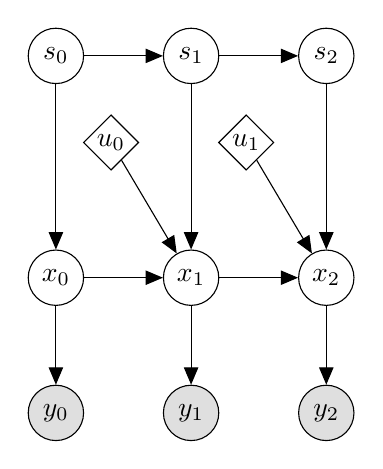
\begin{tikzpicture}

  % Define nodes
  \node[obs] (ya) {$y_0$};
  \node[obs, right=of ya] (yb) {$y_1$};
  \node[obs, right=of yb] (yc) {$y_2$};
  \node[latent, above=of ya]  (xa) {$x_0$};
  \node[latent, above=of yb, right=of xa]  (xb) {$x_1$};
  \node[latent, above=of yc, right=of xb]  (xc) {$x_2$};
  \node[det, above=of xa, xshift=0.7cm] (da) {$u_0$};
  \node[det, above=of xb, xshift=0.7cm] (db) {$u_1$};
  \node[latent, above=of xa, yshift=1.1cm] (sa) {$s_0$};
  \node[latent, above=of xb, yshift=1.1cm] (sb) {$s_1$};
  \node[latent, above=of xc, yshift=1.1cm] (sc) {$s_2$};
  
  % Connect the nodes
  \edge {da} {xb};
  \edge {db} {xc};
  \edge {xa} {ya};
  \edge {xb} {yb};
  \edge {xc} {yc};
  \edge {xa} {xb};
  \edge {xb} {xc};
  \edge {sa} {sb};
  \edge {sb} {sc};
  \edge {sa} {xa};
  \edge {sb} {xb};
  \edge {sc} {xc};
  
\end{tikzpicture}
\caption{Graphical model of this section}
\label{fig_hybridmod1}
\end{figure}
One of the benefits of combining discrete switching variables with linear dynamical models is that it allows us to model nonlinear, even multi-modal, processes with linear models. Intuitively, we can glue together linear models which each describe a nonlinear model in some region and use the switch to determine which one to use. The switch assigns a weight to each model based on its ability to explain the evidence. 

We model this system as follows. Let $s_t \in (1,2,..., M)$ denote a discrete, time homogeneous $M$ state first order Markov chain with transition matrix $P$ as discussed in Section \ref{sec_hmm}. Let each state $s_t=i$ be associated with a parameter set $\left(A_i, B_i, W_i, C_i, V_i \right)$ used to evaluate the dynamical model shown in (\ref{eq_smodel}). If $s_t$ were observed then (\ref{eq_smodel}) would simplify to a set of Latent Linear Dynamical Systems we could perform inference on using the methods investigated in Section \ref{sec_inf_lin_mods}. However, we assume that $s_t$ is a hidden random variable.
\begin{equation}
\begin{aligned}
x_{t+1} &= A_ix_t + B_iu_t + w_{t} \text{ with } \mathcal{N}(w_{t}|0,W_i) \\
y_{t+1} &= C_ix_{t+1} + v_{t+1}  \text{ with } \mathcal{N}(v_{t+1}|0,V_i)
\end{aligned}
\label{eq_smodel}
\end{equation}
To fully specify the system we also require the prior distributions $p(s_0)$ and $p(x_0|s_0)$ as well as the switch transition matrix $P$. For the purposes of this dissertation we assumed that the switch transition matrix is available. This matrix can be inferred using the Baum-Welch Algorithm or it can be set using operator expertise as we will show later.

\subsection{Exact Filtering}
The switching variables ($s_0, s_1, s_2,...$) are discrete random variables exactly like the ones seen in Section \ref{sec_hmm}. There we derived recursive analytic expressions for inference which were computationally inexpensive. The structure of the stochastic variables ($x_0, x_1,x_2,...$) and ($y_0,y_1, y_2,...$) are exactly the same as those found Section \ref{sec_inf_lin_mods}. There we derived the famous Kalman Filter equations which were also analytic, recursive and computationally inexpensive. Taking this into consideration, it seems plausible to believe that inference, specifically filtering, for hybrid systems like (\ref{eq_smodel}) can be formulated in a computationally feasible manner. 

Unfortunately, it can be shown that this is not possible in general \cite{lerner}\cite{murphy3} because the memory requirements scale exponentially with time. Loosely speaking one can see this by noting that at the first time step the system is described by a weighted set of $M$ Kalman Filter models (due to the linear assumption and the $M$ switching indices). At time step two the system is described by a weighted set of $M^2$ Kalman Filter models. Continuing in this manner we see that at time step $t$ the memory requirement is $M^t$. Clearly this is computationally infeasible and calls for approximate methods to be used. 

In literature many approximate filtering algorithms exist and it is not clear which is best. Two of the more popular methods include Gaussian Sum Filtering \cite{barber2} and Particle Filtering based methods (specifically the Rao-Blackwellisation approach, see \cite{chen}\cite{doucet}). Both of these methods take advantage of the Gaussian structure of the system and operate in a fixed memory space making them computationally attractive. We focus on Particle based methods because it can be extended to nonlinear systems with ease.   

\subsection{Rao-Blackwellised Particle Filter}
It is our objective to find the joint posterior distribution $p(s_{0:t}, x_{0:t}|y_{0:t})$. This joint posterior admits filtering of Figure \ref{fig_hybridmod1} if we discard the trajectory and focus only on $s_t,x_t$. By the chain rule (Definition \ref{def_chain_rule_bayes}) we immediately have that $p(s_{0:t}, x_{0:t}|y_{0:t}) = p(s_{0:t}|y_{0:t})p(x_{0:t}|y_{0:t}, s_{0:t})$. Given $s_{0:t}$ we see that $p(x_{0:t}|y_{0:t}, s_{0:t})$ can be evaluated using the Kalman Filter equations (see Section \ref{sec_inf_lin_mods}) and thus we are only concerned with finding some approximation for $p(s_{0:t}|y_{0:t})$. This is the essence of the Rao-Blackwellised Particle Filter - taking advantage of the conditionally linear Gaussian nature of the system to analytically evaluate a part of the posterior distribution \cite{doucet}.

Using the formulation of the adaptive Sequential Importance Sampling algorithm discussed in Section \ref{sec_inf_nonlin_mods} we can apply it to find an approximation of $p(s_{0:t}|y_{0:t})$. We set $\gamma_t(s_{0:t})=p(s_{0:t},y_{0:t})$ and $Z_t=p(y_{0:t})$ and then have that $\frac{\gamma_t(s_{0:t})}{Z_t} = p(s_{0:t}|y_{0:t})$ as desired. We then choose our proposal distribution $q_t(s_{0:t}|y_{0:t})$ to be recursive and follow the same procedure as before, shown in (\ref{eq_rbweight1}).
\begin{equation}
\begin{aligned}
w_t(s_{0:t}) &= \frac{\gamma_t(s_{0:t},y_{0:t})}{q_t(s_{0:t}|y_{0:t})} \\
&= \frac{p(s_{0:t},y_{0:t})}{q_t(s_{0:t}|y_{0:t})} \\
&\propto \frac{p(s_{0:t}|y_{0:t})}{q_t(s_{0:t}|y_{0:t})} \\
&\propto \frac{p(y_t|s_t)p(s_t|s_{t-1})}{q_t(s_t|s_{0:t-1},y_{0:t})}\frac{p(s_{0:t-1}|y_{0:t-1})}{q_t(s_{0:t-1}|y_{0:t-1})} \\
&= \alpha_t(s_{0:t})w_{t-1}(s_{0:t-1})
\end{aligned}
\label{eq_rbweight1}
\end{equation}
As before, we are not interested in the whole trajectory of the switching variable because we only need to perform filtering. Thus our proposal distribution can be chosen to be the prior i.e. $q_t(s_t|s_{0:t-1},y_{0:t}) = p(s_t|s_{t-1})$. This is suboptimal but easy to sample from \cite{doucet}. The incremental weight then simplifies to $\alpha_t(s_{0:t}) = p(y_t|s_t)$. We can evaluate this distribution by marginalising out $x_t$ and using the properties of the Gaussian distributions as before (\ref{eq_rbweight2}).
\begin{equation}
\begin{aligned}
\alpha_t(s_{0:t}) &= p(y_t|s_t) \\
&= \int_{x_t} p(y_t|x_t,s_t)p(x_t|s_{0:t},y_{0:t-1}) \\
&= p(y_t|y_{0:t-1}, s_{0:t}) \\
&= \mathcal{N}\left(y_t | C_{s_t}A_{s_t}\mu_{t-1}, C_{s_t}\left(A_{s_t}\Sigma_{t-1}A_{s_t}^T+Q_{s_t} \right)C_{s_t} + R_{s_t} \right)
\end{aligned}
\label{eq_rbweight2}
\end{equation} 
Where the subscript $s_t$ denotes the state of the switching variable at time $t$ \cite{murphy1}. Upon inspection we see that (\ref{eq_rbweight2}) is just the one step ahead prediction likelihood as discussed in Section \ref{sec_lin_prediction} \cite{murphy1}. Note that we will still need to resample the switching state from $P$ periodically to prevent sample impoverishment. 

We now have an efficient particle approximation of $p(s_t|y_t)$. To find the filtered posterior distribution as desired we note that $p(s_t,x_t|y_{0:t}) = \sum_i w_t(S_t^i)\delta(S_t^i, s_t)p(x_t|y_{0:t}, S_t^i)$ where $S_t^i$ is the i$^{\text{th}}$ particle. Each particle thus consists of a weight, a switch sample and the sufficient statistics generated by the Kalman Filter for a Gaussian i.e. a mean and covariance. The complete algorithm is shown below.

\textbf{Rao-Blackwellised Particle Filter Algorithm}\\
For $t=0$:
\begin{enumerate}
\item
Sample $S^i_0 \backsim p(s_0)$ and $\mu_{0|0}^i \backsim p(x_0|s_0)$.
\item
Compute the weights $w_0(S_0^i) = p(y_0|S_0^i)$ where $y_0$ is the observation. Normalise $W^i_0 \propto w_0(S^i_0)$.
\item
Apply the update step of the Kalman Filter to each particle $i$ and associated parameters to find $\mu_0^i$ and $\Sigma_0^i$. 
\item
If the number of effective particles is below some threshold apply resampling with roughening $(W^i_0, {S}^i_0,{\mu}^i_0, {\Sigma}^i_0)$ to obtain $N$ equally weighted particles $(\frac{1}{N}, \bar{S}^i_0, \bar{\mu}^i_0, \bar{\Sigma}^i_0)$ and set $(\bar{W}^i_0, \bar{S}^i_0, \bar{\mu}^i_0, \bar{\Sigma}^i_0) \leftarrow (\frac{1}{N}, \bar{S}^i_0, \bar{\mu}^i_0, \bar{\Sigma}^i_0)$ otherwise set $(\bar{W}^i_0, \bar{S}^i_0, \bar{\mu}^i_0, \bar{\Sigma}^i_0) \leftarrow ({W}^i_0, {S}^i_0, \mu^i_0, \Sigma_0^i)$
\end{enumerate}
For $t \geq 1$:
\begin{enumerate}
\item
Sample $S^i_t \backsim p(S_t^i|\bar{S}^i_{t-1})$.
\item
Compute the weights $\alpha_t(S^i_{t}) = p(y_t|S_t^i)$ and normalise $W^i_t \propto \bar{W}^i_{t-1}\alpha_t(S^i_{t})$.
\item
Apply the Kalman Filter algorithm to $\mu_{t-1}$ and $\Sigma_{t-1}$ for each particle $i$ to find the sufficient statistics $\mu_{t}$ and $\Sigma_{t}$ using the parameters corresponding to the state of $S^i_t$.
\item
If the number of effective particles is below some threshold apply resampling with roughening $(W^i_t, {S}^i_t,{\mu}^i_t, {\Sigma}^i_t)$ to obtain $N$ equally weighted particles $(\frac{1}{N}, \bar{S}^i_t, \bar{\mu}^i_t, \bar{\Sigma}^i_t)$ and set $(\bar{W}^i_t, \bar{S}^i_t, \bar{\mu}^i_t, \bar{\Sigma}^i_t) \leftarrow (\frac{1}{N}, \bar{S}^i_t, \bar{\mu}^i_t, \bar{\Sigma}^i_t)$ otherwise set $(\bar{W}^i_t, \bar{S}^i_t, \bar{\mu}^i_t, \bar{\Sigma}^i_t) \leftarrow ({W}^i_t, {S}^i_t, \mu^i_t, \Sigma_t^i)$
\end{enumerate} 

\subsection{Rao-Blackwellised Particle Prediction}
Like the Particle Predictor studied in the previous section, performing prediction using Rao-Blackwellisation is straightforward because there is no weighting (updating the particles based on the observation) step. Each particle's switching state is merely propagated forward using the proposal distribution (the transition matrix $P$) and the Kalman prediction algorithm is used to evaluate the predicted mean and covariance. For the sake of brevity we do not supply an algorithm because it is a straightforward simplification of the Rao-Blackwellised Particle Filter Algorithm as shown above. The corresponding Probabilistic Graphical Model is shown in Figure \ref{fig_hybridmod1_prediction}.
\begin{figure}[H] 
\centering
\begin{tikzpicture}

  % Define nodes
  \node[obs] (ya) {$y_0$};
  \node[latent, above=of ya]  (xa) {$x_0$};
  \node[latent, above=of yb, right=of xa]  (xb) {$x_1$};
  \node[latent, above=of yc, right=of xb]  (xc) {$x_2$};
  \node[det, above=of xa, xshift=0.7cm] (da) {$u_0$};
  \node[det, above=of xb, xshift=0.7cm] (db) {$u_1$};
  \node[latent, above=of xa, yshift=1.1cm] (sa) {$s_0$};
  \node[latent, above=of xb, yshift=1.1cm] (sb) {$s_1$};
  \node[latent, above=of xc, yshift=1.1cm] (sc) {$s_2$};
  
  % Connect the nodes
  \edge {da} {xb};
  \edge {db} {xc};
  \edge {xa} {ya};
  \edge {xa} {xb};
  \edge {xb} {xc};
  \edge {sa} {sb};
  \edge {sb} {sc};
  \edge {sa} {xa};
  \edge {sb} {xb};
  \edge {sc} {xc};
  
\end{tikzpicture}
\caption{Rao-Blackwellised Particle Prediction Graphical Model}
\label{fig_hybridmod1_prediction}
\end{figure}

\subsection{Smoothing and Viterbi Decoding}
It is also possible to take advantage of the Gaussian structure in Figure \ref{fig_hybridmod1} to derive a so-called Rao-Blackwellised Smoothing Algorithm. We do not include it here because it is not necessary for the purposes of this dissertation. We refer the reader to the relevant literature \cite{chen}\cite{doucet}. 

Viterbi decoding is likewise not within the scope of this dissertation and as such we refer the reader to \cite{murphy1} for more information. Suffice to say, by increasing the complexity of Figure \ref{fig_hybridmod1} we increase the difficulty of inference in general.

\subsection{Filtering the CSTR}
We now apply the Rao-Blackwellised Particle Filter (RBPF) to the CSTR introduced in Section \ref{sec_cstr}. The focus of this dissertation is on the application of Probabilistic Graphical Models to control, therefore our investigation into the various aspects which improve or degrade filtering performance will be relatively superficial and will target factors which are most relevant only. We will briefly investigate 3 aspects influencing the accuracy of the filter:
\begin{enumerate}
\item
The effect the switch transition matrix $P$ has on the filter.
\item
The effect using more models has on the filter.
\item
Using more state measurements.
\end{enumerate}
Like in Section \ref{sec_inf_nonlin_mods} we do not investigate the effect increasing the number of particles will have on inference. The same reasons apply and we use the same motivation in selecting the number of particles we use in this section.

It should be noted that in all the succeeding investigations only the most probably particle was used to estimate the current state. The reason for this will become clear in Section \ref{sec_rbpf_control} and \ref{sec_spf_control}. It is possible that more accurate state estimates could be reached by using a weighted average of the particles - this approach should be investigated further.

We begin our investigation by only measuring temperature and using 3 linear models, derived by linearising the non-linear CSTR model at each nominal operating point. Since the CSTR has 3 nominal operating points we have 3 linear models. We compare the use of 2 different switch transition matrices $P_1$ and $P_2$ as shown in (\ref{eq_switch_trans}). The first index corresponds to the high temperature operating point ($M_1$), the second index to the unstable operating point ($M_2$) and the third index to the low temperature operating point ($M_3$).
\begin{equation}
\begin{aligned}
P_1 = \begin{pmatrix}
0.50 & 0.25 & 0.25 \\
0.25 & 0.50 & 0.25 \\
0.25 & 0.25 & 0.50
\end{pmatrix} 
~~~&P_2 = \begin{pmatrix}
0.99 & 0.01 & 0.00 \\
0.01 & 0.98 & 0.01 \\
0.00 & 0.01 & 0.99
\end{pmatrix}
\end{aligned}
\label{eq_switch_trans}
\end{equation}
Intuitively $P_1$ indicates that we are less sure about the underlying dynamical transitions i.e. we believe it is possible for the system to jump from the dynamics of the low temperature operating point to the dynamics of the high temperature operating point. Conversely, $P_2$ indicates that we believe it is impossible for the system dynamics to jump from the low temperature operating point to the high temperature operating point without first transitioning through the unstable operating point. 

Figure \ref{fig_3m_models} shows the state space trajectory of the system we are attempting to perform filtering on. The operating points (points of linearisation) are superimposed on the state space.
\begin{figure}[H] 
\centering
\includegraphics[scale=0.25]{rbpf_3m_models.pdf}
\caption{State space of the CSTR problem with the position of the 3 linear models superimposed thereupon. The trajectory followed by the system is also shown, the dot is the initial point and the cross the final point.}
\label{fig_3m_models}
\end{figure}
It is clear from Figure \ref{fig_3m_models} that we expect the filter to use $M_2$ initially and then switch to $M_3$ as time progresses. Figure \ref{fig_3m_vage_track} shows how the RBPF filters the CSTR over a simulation window of 150 minutes. The average concentration error is 21.95\% and the average temperature error is 0.42\% for the state estimator.
\begin{figure}[H] 
\centering
\includegraphics[scale=0.25]{rbpf_3m_vague_track.pdf}
\caption{Filtering with the RBPF using 3 linear models and 500 particles. Switch transition matrix $P_1$ was used.}
\label{fig_3m_vage_track}
\end{figure}
Figure \ref{fig_3m_vage_switch} shows the state of the corresponding switching variable $s_t$ over time. Since $s_t$ is a discrete random variable we have that at each time slice $\sum_{i=1}^{M=3} s_t^i = 1$.
\begin{figure}[H] 
\centering
\includegraphics[scale=0.25]{rbpf_3m_vague_switch.pdf}
\caption{State of the switching variable $s_t$ over time.}
\label{fig_3m_vage_switch}
\end{figure}
From Figure \ref{fig_3m_vage_track} we see that the filtering error is quite large in the unmeasured state. This has been the trend when performing inference on an unmeasured state, however the magnitude of the error does not justify the use of the more complicated Graphical Model. Additionally, we see that there is no clear switching point in Figure \ref{fig_3m_vage_switch} - the filter relies on both $M_2$ an $M_3$ to estimate the state throughout the simulation. This is contrary to what we expected based on Figure \ref{fig_3m_models}.

Figure \ref{fig_3m_track} shows how the RBPF filters the CSTR over a simulation window of 150 minutes using $P_2$. The average concentration error is 5.05\% and the average temperature error is 0.33\% for the state estimator. This is a vast improvement over the case where $P_1$ was used.
\begin{figure}[H] 
\centering
\includegraphics[scale=0.25]{rbpf_3m_track.pdf}
\caption{Filtering with the RBPF using 3 linear models and 500 particles. Switch transition matrix $P_2$ was used.}
\label{fig_3m_track}
\end{figure}
Figure \ref{fig_3m_switch} shows the state of the corresponding switching variable $s_t$ over time.
\begin{figure}[H] 
\centering
\includegraphics[scale=0.25]{rbpf_3m_switch.pdf}
\caption{State of the switching variable $s_t$ over time.}
\label{fig_3m_switch}
\end{figure}
Unlike Figure \ref{fig_3m_vage_switch} we do see a clear model transition around the 20 minute mark in Figure \ref{fig_3m_switch}. This is the behaviour we expected - as the system moves away from the unstable operating point the corresponding Graphical Model becomes less important.

These results suggest that the switch transition matrix sets how ``sticky" the model transitions are. The more vague they are, as in the case of $P_1$, the more unsure the filter is about which model is probably generating the observations. On the other hand, in the case of $P_2$, once the filter switched to the higher probability model it stayed there. This behaviour is desirable because it is easier to base a control strategy off of one model than multiple models. However, the immediate drawback of the ``sticky" approach is that the filter may be over confident. Additionally if a machine learning approach is not used to infer the values of $P$ it could become a tedious task to set $P$ for a large system. Clearly the values used in $P_2$ were set my hand - more investigation is necessary to determine proper heuristics if this approach should be adopted in practice.

Next we investigate the effect of using more models has on the filter. We use the same 3 model filter as before (using $P_2$) but compare it to a 7 model filter. The state transition matrix for the 7 model filter is shown in (\ref{eq_state_trans7}).
\begin{equation}
P_3 = \begin{pmatrix}
0.98 & 0.00 & 0.00 & 0.00 & 0.00 & 0.01 & 0.00 \\
0.00 & 0.98 & 0.00 & 0.01 & 0.01 & 0.01 & 0.00 \\
0.01 & 0.00 & 0.98 & 0.00 & 0.00 & 0.01 & 0.01 \\
0.00 & 0.00 & 0.00 & 0.98 & 0.00 & 0.01 & 0.00 \\
0.00 & 0.01 & 0.00 & 0.00 & 0.99 & 0.00 & 0.00 \\
0.01 & 0.01 & 0.01 & 0.01 & 0.00 & 0.96 & 0.00 \\
0.00 & 0.00 & 0.01 & 0.00 & 0.00 & 0.00 & 0.99 \\
\end{pmatrix}
\label{eq_state_trans7}
\end{equation}
The values of $P_3$ were set using the same reasoning as before. Figure \ref{fig_7m_models} show state trajectory of the system (like Figure \ref{fig_3m_models}) but with the additional models superimposed thereupon.
\begin{figure}[H] 
\centering
\includegraphics[scale=0.25]{rbpf_7m_models.pdf}
\caption{State space of the CSTR problem with the position of the 3 linear models superimposed thereupon. The trajectory followed by the system is also shown, the dot is the initial point and the cross the final point.}
\label{fig_7m_model}
\end{figure}


\chapter{Stochastic switching linear control using linear hybrid models}
\label{sec_rbpf_control}
In section \ref{sec_switch_mpc_lit} model switching MPC was introduced. In short, a set of models with corresponding binary integer variables are incorporated into the MPC optimisation problem. The optimisation algorithm changes the model it uses for prediction based on the location of the previous predicted state. In this way a number of models can potentially be used for prediction. It is desirable to change models if the system states move far away from the linearisation point of current linear model. It is hoped that the significant computational burden this introduces is offset by the increased predictive accuracy of the controller.

In chapter \ref{sec_linear_control} we developed efficient stochastic controller algorithms (LQG and MPC) which use a single linear model for control. While it is possible to attempt to extend these algorithms to the aforementioned approach, the computational problems will persist because mixed integer programming is fundamentally more difficult than quadratic programming \cite{forst}. From a practical perspective one would like to reduce computational complexity because, especially for large problems, on-line optimisation can become problematic.

In chapter \ref{sec_inf_lin_hybrid} the Rao-Blackwellised particle filter was introduced. Briefly, the filter uses a set of linear models, $M_i=(A_i, B_i)$ for each model $i$, to estimate the current state (we assume the system and measurement noise is common across all models as well as the observation matrix). The ability of each model to explain the observations is calculated in a Bayesian sense. This is used to weight the importance of each model's contribution to the current state estimate. 

In this chapter we will attempt to combine the ideas of section \ref{sec_switch_mpc_lit}, and chapters \ref{sec_linear_control} and \ref{sec_inf_lin_hybrid} to create a computationally efficient switching model controller algorithm. We assume that the underlying process dynamics are described by
\begin{equation}
\begin{aligned}
x_{t+1} &= f(x_t, u_t) + w_{t+1}  \\
y_{t+1} &= g(x_{t+1}) + v_{t+1}  
\end{aligned}
\label{eq_lin_system_in_rbpf}
\end{equation}
where $f$ and $g$ are the nonlinear transition and observation functions of the CSTR process introduced in chapter \ref{sec_cstr}. It is assumed that $x_t$ is a latent stochastic variable and $y_t$ is an observed stochastic variable. We also assume that the models used for inference and control are linear and of the form 
\begin{equation}
\begin{aligned}
x_{t+1} &= A_ix_t + B_iu_t + w_{t+1} \\
y_{t+1} &= Cx_{t+1} + v_{t+1} 
\end{aligned}
\label{eq_lin_system_control_rbpf}
\end{equation}
for model $M_i=(A_i, B_i)$. The noise terms retain their meaning from chapter \ref{sec_linear_control}. It is our aim to move the system states from the  unstable (nominal) operating point to another operating point. This will clearly cause the system to traverse the state space and necessitate model switching. We first describe the intuition behind the proposed switching controller algorithm and then state the algorithm.

As mentioned before, it becomes desirable to have a mechanism to switch the underlying controller model if the system states move far away from the linearisation point of the current model. However, it is computationally difficult to perform this switching within the framework of the optimisation algorithm because it invariably necessitates the introduction of integer variables. We propose an algorithm which uses the Rao-Blackwellised particle filter to estimate the current state as well as the models which best describe the current observation. Based on the results of chapter \ref{sec_inf_lin_hybrid} we expect the weight assigned to each model to skew in favour of the models which were linearised closest to the current state. Now we have two options to implement control at each time step\footnote{Note that $A^*$ is the model used for control in this explanation.}:
\begin{enumerate}
\item
Use only the most likely model (the model with the highest switch weight) for controller prediction i.e. use $A^* = A_{\text{indmax}[s_t]}$. See section \ref{sec_rbpf_control_uncon}.
\item
Use the weighted average (from the switch weight) of the models for controller prediction i.e. use $A^* = \sum_{i=1}^M s_t^i A_i$. See section \ref{sec_ma_rbpf}.
\end{enumerate}
Since it is not clear which approach is best we investigate both. This ``best current model" is then used in the single model controller algorithms discussed in chapter \ref{sec_linear_control}. This approach falls squarely between the purely single model controllers, as discussed in chapter \ref{sec_linear_control}, and the switching model controllers, where the model switching occurs inside the optimisation problem, as discussed in section \ref{sec_switch_mpc_lit}. By switching models outside the optimisation problem the scheme will necessarily be more computationally efficient than those found in section \ref{sec_switch_mpc_lit}. 

\textbf{Switching controller algorithm}:
\begin{enumerate}
\item
Use a switching filter algorithm, e.g. the Rao-Blackwellised particle filter, to update the state estimates of the particle population given the current observation. See chapter \ref{sec_inf_lin_hybrid} for more details.
\item
Select the best current model to for control based on the model weights also supplied by the switching filter algorithm.
\item
Use the mean and covariance information from the current posterior state estimate and the best current model (from step 2) within the context of the stochastic controller (LQG or MPC) formulation of chapter \ref{sec_linear_control}.
\item
Repeat for the next observation. 
\end{enumerate} 
The astute reader will notice that we are implicitly using the graphical model shown in figure~\ref{fig_gm_filter} for state estimation (filtering) but the graphical model of figure \ref{fig_gm_prediction} for model based prediction in step 3.
\begin{figure}[H] 
\centering
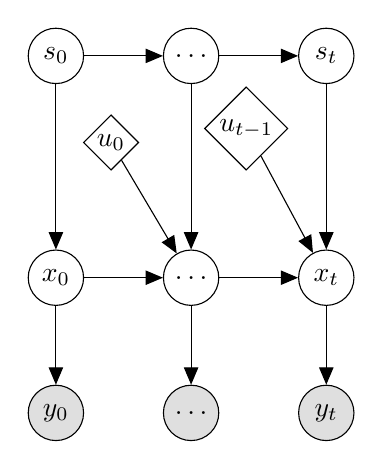
\begin{tikzpicture}

  % Define nodes
  \node[obs] (ya) {$y_{0}$};
  \node[obs, right=of ya] (yb) {${\hdots}$};
  \node[obs, right=of yb] (yc) {$y_{t}$};
  \node[latent, above=of ya]  (xa) {$x_{0}$};
  \node[latent, above=of yb, right=of xa]  (xb) {${\hdots}$};
  \node[latent, above=of yc, right=of xb]  (xc) {$x_{t}$};
  \node[det, above=of xa, xshift=0.7cm] (da) {$u_{0}$};
  \node[det, above=of xb, xshift=0.7cm] (db) {$u_{t-1}$};
  \node[latent, above=of xa, yshift=1.1cm] (sa) {$s_{0}$};
  \node[latent, above=of xb, yshift=1.1cm] (sb) {${\hdots}$};
  \node[latent, above=of xc, yshift=1.1cm] (sc) {$s_{t}$};
  
  % Connect the nodes
  \edge {da} {xb};
  \edge {db} {xc};
  \edge {xa} {ya};
  \edge {xb} {yb};
  \edge {xc} {yc};
  \edge {xa} {xb};
  \edge {xb} {xc};
  \edge {sa} {sb};
  \edge {sb} {sc};
  \edge {sa} {xa};
  \edge {sb} {xb};
  \edge {sc} {xc};
  
\end{tikzpicture}
\caption{Graphical model used for state estimation.}
\label{fig_gm_filter}
\end{figure}
\begin{figure}[H] 
\centering
\begin{tikzpicture}

  % Define nodes
  \node[obs] (ya) {$y_0$};
  \node[latent, above=of ya]  (xa) {$x_0$};
  \node[latent, above=of yb, right=of xa]  (xb) {$x_1$};
  \node[latent, above=of yc, right=of xb]  (xc) {$x_2$};
  \node[det, above=of xa, xshift=0.7cm] (da) {$u_0$};
  \node[det, above=of xb, xshift=0.7cm] (db) {$u_1$};
  \node[latent, above=of xa, yshift=1.1cm] (sa) {$s_0$};
  
  % Connect the nodes
  \edge {da} {xb};
  \edge {db} {xc};
  \edge {xa} {ya};
  \edge {xa} {xb};
  \edge {xb} {xc};
  \edge {sa} {xa};
\end{tikzpicture}
\caption{Simplified graphical model used for prediction. Within the context of prediction we have that $x_0 \leftarrow x_t$ and $s_0 \leftarrow s_t$ at each successive time step to simplify notation.}
\label{fig_gm_prediction}
\end{figure}
We are not using the graphical model associated with Rao-Blackwellised particle prediction (see section \ref{sec_inf_rbpf_pred}) because that would require that we incorporate stochastic model switching within the optimisation algorithm. 

For the remainder of this chapter we assume that we have a bank of $M$ linear models and that we measure both states. Each model is derived by linearising the non-linear CSTR model, found in chapter \ref{sec_cstr}, around the nominal operating points discussed in the same chapter as well as section \ref{sec_rbpf_filtering_cstr}. We also use the switching transition matrices $P_2, P_3$ found in (\ref{eq_switch_trans}) where appropriate. All other parameters are the same as those found in chapter \ref{sec_linear_control}.
\section{Unconstrained switching control}
As mentioned earlier, we will investigate two approaches which can be used to implement the switching controller algorithm. The first approach, used in section \ref{sec_rbpf_control_uncon}, makes use of only the most likely model within the controller. The second approach, discussed in section \ref{sec_ma_rbpf}, makes use of model averaging to construct a model for control.  
\subsection{Most likely model approach}
\label{sec_rbpf_control_uncon}
Due to the analysis of section \ref{sec_uncon_lin_control} we know that it is possible to convert the stochastic optimisation problem
\begin{equation}
\begin{aligned}
&\underset{\mathbf{u}}{\text{min }} \mathbb{E}\left[ \frac{1}{2}\sum_{k=0}^{N-1} \left( x_k^TQx_k + u_k^TRu_k \right) + \frac{1}{2}x_N^TP_fx_N \right] \\
& \text{subject to } x_{t+1}=A_ix_t+B_iu_t + w_t\\
\end{aligned}
\label{eq_rbpf_lqg}
\end{equation}
into the deterministic optimisation problem
\begin{equation}
\begin{aligned}
&\underset{\mathbf{u}}{\text{min }} \frac{1}{2}\sum_{k=0}^{N-1} \left( \mu_k^TQ\mu_k + u_k^TRu_k \right) + \frac{1}{2}\mu_N^TP_f\mu_N + \frac{1}{2}\sum_{k=0}^N \text{tr}(Q\Sigma_k) \\
&\text{with } \mu_{t+1} = A_i\mu_t +B_iu_t \\
&\text{and } \Sigma_{t+1} = W+A_i\Sigma_t A_i^T 
\end{aligned}
\label{eq_rbpf_lqr}
\end{equation}
for each linear model $(M_1, M_2, M_3)$ given that we have the current state estimate $x_0$, the model dynamics are linear and the underlying distributions are Gaussian. Throughout this chapter we make these assumptions\footnote{Note that the underlying model is clearly nonlinear but the model used for prediction and inference is linear.}. As before, we also denote the mean and covariance of the current state estimate $x_0$ by $\mathbb{E}[x_0]=\mu_0$ and $\text{var}[x_0]=\Sigma_0$. We use a prediction horizon of $N=150$ i.e. 15 minutes into the future.
We have that (\ref{eq_rbpf_lqg}) is equivalent to (\ref{eq_rbpf_lqr}) under the aforementioned assumptions.

Given this we apply the switching controller algorithm within the context of the LQG controller i.e. given a model $M_i$ from the filter we solve the LQG problem and implement that input. In light of our analysis in chapter \ref{sec_linear_control} it is clear that the switching controller algorithm is straightforward to implement because it simplifies to $M$ deterministic LQR controllers.

As mentioned before we only use the most likely model for control purposes here. By only selecting one model to use for control we dramatically simplify the control problem. It allows us to use the controllers of chapter \ref{sec_linear_control} directly. 

We study 4 control problems using the switching controller algorithm in this chapter. Problems 1 and 2 allow the controller to switch between 3 linear models and problems 3 and 4 allow the controller to switch between 7 linear models. Furthermore, problems 1 and 3 seek to drive the system to the low temperature operating point i.e. a concentration set point of $0.998~\text{kmol.m}^{-3}$ while problems 2 and 4 seek to drive the CSTR to a concentration set point of $0.90~\text{kmol.m}^{-3}$. In all cases we use the switching LQG controller as shown in (\ref{eq_rbpf_lqg}).

We investigate the first problem in figures \ref{fig_rbpf_control_state} to \ref{fig_rbpf_control_track}. In figure \ref{fig_rbpf_control_state} we see the state space trajectory of the system under control. We expect $M_2$ to be active initially after which only $M_3$ should be active.
\begin{figure}[H] 
\centering
\includegraphics[width=\textwidth]{rbpf_control_state.pdf}
\caption{State space trajectory of the non-linear CSTR under control of the LQG switching controller algorithm. The initial point was $(0.49, 412)$}
\label{fig_rbpf_control_state}
\end{figure}
Figure \ref{fig_rbpf_control_switch} confirms the behaviour we expected: initially $M_2$ best explained the observations but $M_2$ gives way to $M_3$ throughout the rest of the simulation.   
\begin{figure}[H] 
\centering
\includegraphics[width=\textwidth]{rbpf_control_switch.pdf}
\caption{Most likely model used for control at each time step over the simulation. Black indicates the model is active.}
\label{fig_rbpf_control_switch}
\end{figure}
However, it is clear that there are some problems in figure \ref{fig_rbpf_control_switch}. There does seem to be some slight switching noise. Given that we are using the sticky switching transition matrix $P_2$ it is clear that model overlap is causing problems. The same problem was identified in section \ref{sec_rbpf_filtering_cstr}. In figure \ref{fig_rbpf_control_track} we see the set point tracking performance of the switching controller. It is clear that the controller tracks the set point.
\begin{figure}[H] 
\centering
\includegraphics[width=\textwidth]{rbpf_control_track.pdf}
\caption{Set point tracking and controller input for the LQG 3 model switching controller algorithm. The initial point was $(0.49, 412)$.}
\label{fig_rbpf_control_track}
\end{figure}
Based on figures \ref{fig_rbpf_control_switch} and \ref{fig_rbpf_control_track} it would be too easy to surmise that the controller algorithm works. Unfortunately this is not the case in general. In figures \ref{fig_rbpf_control_switch2} and \ref{fig_rbpf_control_track2} we study problem 2: tracking the concentration set point of $0.90~\text{kmol.m}^{-3}$. In figure \ref{fig_rbpf_control_switch2} we see significant model switching noise.
\begin{figure}[H] 
\centering
\includegraphics[width=\textwidth]{rbpf_control_switch2.pdf}
\caption{Most likely model used for control at each time step over the simulation. Black indicates the model is active.}
\label{fig_rbpf_control_switch2}
\end{figure}
In figure \ref{fig_rbpf_control_track2} the detrimental consequence of the switching noise is evident. The controller is completely unstable and oscillates.
\begin{figure}[H] 
\centering
\includegraphics[width=\textwidth]{rbpf_control_track2.pdf}
\caption{Set point tracking and controller input for the LQG 3 model switching controller algorithm. The initial point was $(0.49, 412)$.}
\label{fig_rbpf_control_track2}
\end{figure}
It is clear that the oscillations are caused by the filter's inability to stick to a model. There are two major problems with the switching controller algorithm as adopted in this chapter:
\begin{enumerate}
\item
Fundamentally we are using an inappropriate model for controller prediction during the initial period of the simulation. If we stayed near the current position in state space then the most likely model would predict the future well and thus result in good control. However, we are projecting the controlled states into regions where the current model control is based upon may not a good approximation at all. This is a fundamental problem of our approach - it would be better to incorporate the model switching within the controller prediction (optimisation) process, but this is exactly what we want to avoid due to the computational burden this introduces!
\item
The switching noise is problematic because it can cause the controller to use a model which is good locally (for the current observation) but inappropriate with regard to the true underlying position of the system in state space. However, from an inference perspective the noise is not necessarily undesirable. Switching noise can improve the state estimate accuracy - especially in regions between models. It is also important in allowing the filter to switch punctually: making the switching transition matrix too static retards the sensitivity the filter has to model changes. It is possible to address the issue of switching noise without making the switch transition matrix too static. The augmented switching filter model, shown in figure \ref{fig_gm_augmented}, is a candidate for this.
\begin{figure}[H] 
\centering
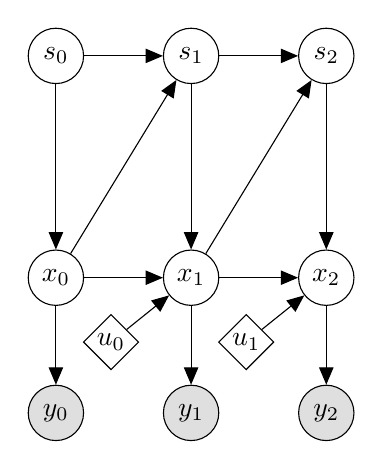
\begin{tikzpicture}

  % Define nodes
  \node[obs] (ya) {$y_{0}$};
  \node[obs, right=of ya] (yb) {$y_{1}$};
  \node[obs, right=of yb] (yc) {$y_{2}$};
  \node[latent, above=of ya]  (xa) {$x_{0}$};
  \node[latent, above=of yb, right=of xa]  (xb) {$x_{1}$};
  \node[latent, above=of yc, right=of xb]  (xc) {$x_{2}$};
  \node[det, below=of xa, xshift=0.7cm, yshift=0.9cm] (da) {$u_{0}$};
  \node[det, below=of xb, xshift=0.7cm, yshift=0.9cm] (db) {$u_{1}$};
  \node[latent, above=of xa, yshift=1.1cm] (sa) {$s_{0}$};
  \node[latent, above=of xb, yshift=1.1cm] (sb) {$s_{1}$};
  \node[latent, above=of xc, yshift=1.1cm] (sc) {$s_{2}$};
  
  % Connect the nodes
  \edge {da} {xb};
  \edge {db} {xc};
  \edge {xa} {ya};
  \edge {xb} {yb};
  \edge {xc} {yc};
  \edge {xa} {xb};
  \edge {xb} {xc};
  \edge {sa} {sb};
  \edge {sb} {sc};
  \edge {sa} {xa};
  \edge {sb} {xb};
  \edge {sc} {xc};
  \edge {xa} {sb};
  \edge {xb} {sc};
    
\end{tikzpicture}
\caption{Augmented switching filter graphical model.}
\label{fig_gm_augmented}
\end{figure}
Using this model it is possible to model the influence the state variables $(x_0,x_1,...)$ have on the switching variables $(s_0, s_1,...)$. Plausibly this could ameliorate switching noise while not making the switching transition matrix too sticky. For example, the switch transition matrix could, in this case, be a function of the location of the current system state. However, since this would require that we modify the graphical model of figure~\ref{fig_gm_filter} we leave it for future work.
\end{enumerate}
We rather attempt to ameliorate these problems by extending the number of models available to the filter. We use more models to bridge the gap between the current most likely model and where it projects the states during prediction. In figure \ref{fig_rbpf_control_state3} we illustrate the state space trajectory followed by the system when it has 7 models available for inference and control.
\begin{figure}[H] 
\centering
\includegraphics[width=\textwidth]{rbpf_control_state3.pdf}
\caption{State space trajectory of the non-linear CSTR under control of the LQG 7 model switching controller algorithm. The initial point was $(0.49, 412)$}
\label{fig_rbpf_control_state3}
\end{figure}
In figures \ref{fig_rbpf_control_switch3} and \ref{fig_rbpf_control_track3} we again attempt to steer the system from the unstable operating point to the low temperature operating point. Figure \ref{fig_rbpf_control_switch3} shows which models were active over the simulation window.
\begin{figure}[H] 
\centering
\includegraphics[width=\textwidth]{rbpf_control_switch3.pdf}
\caption{Most likely model used for control at each time step over the simulation. Black indicates the model is active.}
\label{fig_rbpf_control_switch3}
\end{figure}
While there is slight switching noise the model selection is exactly what one would expect. Figure \ref{fig_rbpf_control_track3} shows the controller set point tracking performance over the simulation window.
\begin{figure}[H] 
\centering
\includegraphics[width=\textwidth]{rbpf_control_track3.pdf}
\caption{Set point tracking and controller input for the LQG 7 model switching controller algorithm. The initial point was $(0.49, 412)$.}
\label{fig_rbpf_control_track3}
\end{figure}
Like figure \ref{fig_rbpf_control_track} we also have a stable, reference tracking controller. This is not surprising because the model switching/selection was reasonable. In figure \ref{fig_rbpf_control_switch4} and \ref{fig_rbpf_control_track4} we again attempt to steer the system to a concentration set point of $0.9$ kmol.m$^{-3}$. Since we introduced $M_3$ to serve as a bridge between $M_6$ and $M_7$ (since the set point is between these two models) we expect better performance than in figure \ref{fig_rbpf_control_switch2} and \ref{fig_rbpf_control_track2}. Unfortunately this is not the case as may be seen in figures \ref{fig_rbpf_control_switch4} and \ref{fig_rbpf_control_track4}.
\begin{figure}[H] 
\centering
\includegraphics[width=\textwidth]{rbpf_control_switch4.pdf}
\caption{Most likely model used for control at each time step over the simulation. Black indicates the model is active.}
\label{fig_rbpf_control_switch4}
\end{figure}
The same oscillating switching noise and unstable control is present here as there was in figures \ref{fig_rbpf_control_switch2} and \ref{fig_rbpf_control_track2}.
\begin{figure}[H] 
\centering
\includegraphics[width=\textwidth]{rbpf_control_track4.pdf}
\caption{Set point tracking and controller input for the LQG 7 model switching controller algorithm. The initial point was $(0.49, 412)$.}
\label{fig_rbpf_control_track4}
\end{figure}
The underlying reasons for the instability are the same: we are using models to predict into regions where they are inaccurate and the filter does not robustly enough isolate the model closest to the current system location in state space. The combination of these two problems make effective control impossible.

\subsection{Model averaging approach}
\label{sec_ma_rbpf}
The fundamental problem with the switching controllers of section \ref{sec_rbpf_control_uncon} is that an inappropriate model was used for prediction. Unfortunately using a weighted average of all the models, based on their probability with respect to the switching variable $s_t$, will exacerbate this problem. For this reason we do not explore this approach.

\section{Conclusion}
The goal of the switching controller algorithm was to drastically reduce the computational burden introduced by modern switching controller implementations as discussed in section~\ref{sec_switch_mpc_lit}. The approach of switching the model used for control outside the optimisation algorithm, while attractive intuitively, suffers from the fundamental problem that a bad model is used to predict the future states.

The switching LQG controllers introduced in this chapter were not robust against this type of problem. Additionally, we also had severe switching noise which led to controller oscillation. From a fundamental point of view it seems as if the current approach of incorporating the model switching inside the optimisation algorithm has the most promise of yielding good control. 

It should be investigated whether it is feasible to incorporate the Rao-Blackwellised particle prediction (see section \ref{sec_inf_rbpf_pred}) within the controller optimisation process.  
\chapter{Inference using nonlinear hybrid models}
\label{sec_inf_spf}
In this chapter we study the same graphical model as Chapter \ref{sec_inf_lin_hybrid}, shown in Figure \ref{fig_hybridmod2} for convenience, but we drop the assumption that the dynamic models used for inference are linear. The variables retain their meaning as before.     
\begin{figure}[H] 
\centering
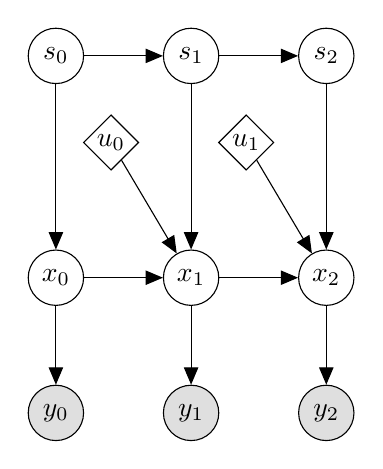
\begin{tikzpicture}

  % Define nodes
  \node[obs] (ya) {$y_0$};
  \node[obs, right=of ya] (yb) {$y_1$};
  \node[obs, right=of yb] (yc) {$y_2$};
  \node[latent, above=of ya]  (xa) {$x_0$};
  \node[latent, above=of yb, right=of xa]  (xb) {$x_1$};
  \node[latent, above=of yc, right=of xb]  (xc) {$x_2$};
  \node[det, above=of xa, xshift=0.7cm] (da) {$u_0$};
  \node[det, above=of xb, xshift=0.7cm] (db) {$u_1$};
  \node[latent, above=of xa, yshift=1.1cm] (sa) {$s_0$};
  \node[latent, above=of xb, yshift=1.1cm] (sb) {$s_1$};
  \node[latent, above=of xc, yshift=1.1cm] (sc) {$s_2$};
  
  % Connect the nodes
  \edge {da} {xb};
  \edge {db} {xc};
  \edge {xa} {ya};
  \edge {xb} {yb};
  \edge {xc} {yc};
  \edge {xa} {xb};
  \edge {xb} {xc};
  \edge {sa} {sb};
  \edge {sb} {sc};
  \edge {sa} {xa};
  \edge {sb} {xb};
  \edge {sc} {xc};
  
\end{tikzpicture}
\caption{Graphical model of this chapter.}
\label{fig_hybridmod2}
\end{figure}
Intuitively we are now using the switching variables to decide which nonlinear model (or combination of) better describes the observed system behaviour. At each point in time we desire a weighted set of nonlinear models with the weight proportional to the ability of the model to explain the plant behaviour. Such a system could be used to describe significant model changes e.g. catalyst degradation in our CSTR or a reactor which breaks suddenly etc... 

We model this system as follows. Let $s_t$ denote a discrete $M$ state first order Markov chain with transition matrix $P$ as discussed in Chapter \ref{sec_inf_lin_hybrid}. Let each state $s_t=i$ be associated with a model set $\left(f_i, g_i, W_i, V_i \right)$ used to evaluate the dynamical model shown in (\ref{eq_smodel2}).
\begin{equation}
\begin{aligned}
x_{t+1} &= f_i(x_t, u_t, w_{t+1}) \text{ with } w_{t+1} \backsim \mathcal{N}(0, W_i)\\
y_{t+1} &= g_i(x_{t+1}, v_{t+1}) \text{ with } v_{t+1} \backsim \mathcal{N}(0,V_i)
\end{aligned}
\label{eq_smodel2}
\end{equation}
In this dissertation we assume that the the noise distributions are Gaussian but there is no fundamental reason why they cannot be arbitrary. To fully specify the system we again require the prior distributions $p(s_0)$ and $p(x_0|s_0)$ as well as the stochastic matrix $P$. In this chapter we manually specify the matrix $P$ but it can be computed using the Baum-Welch algorithm. 
\section{Exact filtering}
By extending the model to incorporate nonlinear models it becomes even more difficult to perform inference. It is clear that for the type of systems we consider here no exact inference algorithm, which is computationally feasible, exists \cite{murphy1}. We again turn to approximate inference algorithms.

Note that we cannot apply Rao-Blackwellisation (i.e. analytically evaluate the stochastic dynamical system component and approximate the switching component) as before because the dynamic models used for inference are no longer linear. We use the adaptive sequential importance resampling, i.e. the bootstrap particle filter, algorithm as discussed in Chapter \ref{sec_inf_nonlin_mods}.
\section{Switching particle filter}
We cannot analytically evaluate any part of the desired posterior distribution $p(s_{0:t}, x_{0:t}|y_{0:t})$ in a computationally feasible manner, so we must apply the adaptive sequential importance resampling algorithm to the entire state space of Figure \ref{fig_hybridmod2}. The algorithm follows straightforwardly from our discussion in Chapter \ref{sec_asir} \cite{murphy1}. We merely state the proposal distribution and incremental weight function we sample from in (\ref{eq_nonpf}). 
\begin{equation}
\begin{aligned}
&q_t(s_t,x_t|s_{0:t-1},x_{0:t-1,}y_{0:t}) = p(s_t|s_{t-1})p(x_t|s_t,x_{t-1}) \\
&\alpha_t(s_{0:t},x_{0:t}) = p(y_t|x_t,s_t)
\end{aligned}
\label{eq_nonpf}
\end{equation}  
Applying the algorithm is a straightforward extension of the bootstrap particle filter introduced in Chapter \ref{sec_bootstrap} given the weighting function and proposal distribution as shown below.

\textbf{Switching particle filter algorithm}\\
For $t=0$:
\begin{enumerate}
\item
Sample $S^i_0 \backsim p(s_0)$ and $X^i_0 \backsim p(x_0|s_0)$.
\item
Compute the weights $w_0(S_0^i, X_0^i) = p(y_0|S_0^i, X_0^i)$ where $y_0$ is the observation. Normalise $W^i_0 \propto w_0(S_0^i, X_0^i)$. 
\item
If the number of effective particles is below some threshold apply resampling with roughening $(W^i_0, S^i_0, X^i_0)$ to obtain $N$ equally weighted particles $(\frac{1}{N}, \bar{S}^i_0, \bar{X}^i_0)$ and set $(\bar{W}^i_0, \bar{S}^i_0,\bar{X}^i_0) \leftarrow (\frac{1}{N}, \bar{S}^i_0, \bar{X}^i_0)$ otherwise set $(\bar{W}^i_0,\bar{S}^i_0, \bar{X}^i_0) \leftarrow ({W}^i_0, S_0^i, {X}^i_0)$
\end{enumerate}
For $t \geq 1$:
\begin{enumerate}
\item
Sample $S^i_t \backsim p(S_t^i|\bar{S}^i_{t-1})$ and $X^i_t \backsim p(X^i_t|S^i_t, \bar{X}^i_{t-1})$.
\item
Compute the weights $\alpha_t(S_t^i, X_t^i) = p(y_t|S_t^i, X_t^i)$ where $y_t$ is the observation. Normalise $W^i_t \propto W^i_{t-1}\alpha_t(S_t^i, X_t^i)$.
\item
If the number of effective particles is below some threshold apply resampling with roughening $(W^i_t, S^i_t, X^i_t)$ to obtain $N$ equally weighted particles $(\frac{1}{N}, \bar{S}^i_t, \bar{X}^i_t)$ and set $(\bar{W}^i_t, \bar{S}^i_t,\bar{X}^i_t) \leftarrow (\frac{1}{N}, \bar{S}^i_t, \bar{X}^i_t)$ otherwise set $(\bar{W}^i_t,\bar{S}^i_t, \bar{X}^i_t) \leftarrow ({W}^i_t, S_t^i, {X}^i_t)$
\end{enumerate} 

\section{Switching particle prediction}
The prediction of the hybrid nonlinear states follows in an analogous manner to the prediction algorithm found in Chapter \ref{sec_particle_prediction}. We do not supply an algorithm because it is a straightforward simplification of the switching particle filter algorithm seen above: effectively there is no weight update step because there is no observation. The corresponding graphical model is shown in Figure \ref{fig_hybridmod2_prediction}.
\begin{figure}[H] 
\centering
\begin{tikzpicture}

  % Define nodes
  \node[obs] (ya) {$y_0$};
  \node[latent, above=of ya]  (xa) {$x_0$};
  \node[latent, above=of yb, right=of xa]  (xb) {$x_1$};
  \node[latent, above=of yc, right=of xb]  (xc) {$x_2$};
  \node[det, above=of xa, xshift=0.7cm] (da) {$u_0$};
  \node[det, above=of xb, xshift=0.7cm] (db) {$u_1$};
  \node[latent, above=of xa, yshift=1.1cm] (sa) {$s_0$};
  \node[latent, above=of xb, yshift=1.1cm] (sb) {$s_1$};
  \node[latent, above=of xc, yshift=1.1cm] (sc) {$s_2$};
  
  % Connect the nodes
  \edge {da} {xb};
  \edge {db} {xc};
  \edge {xa} {ya};
  \edge {xa} {xb};
  \edge {xb} {xc};
  \edge {sa} {sb};
  \edge {sb} {sc};
  \edge {sa} {xa};
  \edge {sb} {xb};
  \edge {sc} {xc};
  
\end{tikzpicture}
\caption{Switching particle prediction graphical model.}
\label{fig_hybridmod2_prediction}
\end{figure}  

\section{Smoothing and Viterbi decoding}
Like Chapter \ref{sec_inf_lin_hybrid} we refer the reader elsewhere for a detailed discussion on both smoothing and Viterbi decoding \cite{murphy1}. It suffices to say that given the nonlinear dynamics the aforementioned inference will be beyond the scope of this dissertation. 

\section{Filtering the CSTR}
\label{sec_spf_filtering}
In this chapter we illustrate the use of the switching particle filter using  two nonlinear dynamical model derived from the familiar CSTR example of Chapter \ref{sec_cstr}. Since the graphical model of Chapter \ref{sec_inf_lin_hybrid} is identical to that of Figure \ref{fig_hybridmod2} we expect that the general trends discussed in Chapter \ref{sec_rbpf_filtering_cstr} to hold here as well.

For the purposes of illustration we assume a scenario where the rate constant of the CSTR decreases by an order of magnitude. This scenario is not completely arbitrary, for example, this could be caused by catalyst degradation due to some environmental factor. It is our aim to infer when this happens and to be able to track the states accurately despite the significant model change. Therefore we will have one nonlinear model of the healthy plant $M_1$ and one nonlinear model of the faulty plant $M_2$.

Note that the character of the inference we are attempting to do is fundamentally different from that of Chapter \ref{sec_inf_lin_hybrid} but that the underlying graphical models are the same. In Chapter \ref{sec_inf_lin_hybrid} the Rao-Blackwellised particle filter switched between models which all attempt to describe the same physical system albeit in different regions of the state space. In this chapter the switching particle filter will attempt to switch between models which describe completely different physical systems. This difference informs our choice of the switch transition matrix.

We use 500 particles during all runs for the switching particle filter and use the switching transition matrix $P_1=\begin{pmatrix}
0.99 & 0.01 \\ 0.01 & 0.99
\end{pmatrix}$. For the particle filter, used for a comparative base, we use 200 particles. We spent much time in Chapter \ref{sec_rbpf_filtering_cstr} discussing the effect the switch transition matrix has on model selection. The form of the matrix is motivated by physical considerations as well: once the catalyst denatures it is unlikely to fix itself. Thus, once the model breaks, switches from $M_1$ to $M_2$, it is unlikely to switch back. In all the simulations the catalyst denatures at 50 minutes into the run.

We conduct two brief, but illustrative, investigations comparing the effectiveness of the switching particle filter and the particle filter. In both cases the particle filter uses the healthy system model - the benefit of the additional complexity of the switching particle filter model is to be highlighted here. In the first investigation we measure only temperature and in the second we measure both concentration and temperature. 

In Figure \ref{fig_pf_m1_compspf} we illustrate the tracking performance\footnote{Unfortunately we cannot use the average tracking performance measures used previously. Since the filter approaches a concentration of 0 $\text{kmol.m}^{-3}$ the average error estimates are not accurate: there is division by very small numbers. We thus rely on a visual comparison.} of the particle filter on the system. Note that the simulation window is very long - 600 minutes.
\begin{figure}[H] 
\centering
\includegraphics[width=\textwidth]{pf_m1_compspf.pdf}
\caption{Particle filter using 200 particles tracking the CSTR where the catalyst denatures at 50 minutes. Only temperature is measured.}
\label{fig_pf_m1_compspf}
\end{figure}
It is clear that the particle filter tracks the temperature well, because it is measured, but tracks the concentration very poorly. It takes almost 300 minutes before the particle filter estimates the concentration reliably. Clearly the model mismatch causes the filter's poor performance - compare this to the excellent tracking in Chapter \ref{sec_nonlinmods_filtering}.

In Figure \ref{fig_spf_m1_track} we see the tracking performance of the switching particle filter measuring only temperature.
\begin{figure}[H] 
\centering
\includegraphics[width=\textwidth]{spf_m1_track.pdf}
\caption{switching particle filter using 500 particles tracking the CSTR where the catalyst denatures at 50 minutes.}
\label{fig_spf_m1_track}
\end{figure}
It is clear that the switching particle filter tracks the states very well. However, Figure \ref{fig_spf_m1_switch} indicates that we have the some switching noise problems.
\begin{figure}[H] 
\centering
\includegraphics[width=\textwidth]{spf_m1_switch.pdf}
\caption{Switching particle filter measuring only temperature. The switching weight of each particle is shown per time step. $M_1$ corresponds to the healthy plant and $M_2$ to the broken plant.}
\label{fig_spf_m1_switch}
\end{figure} 
It is not surprising that there is switching noise: the graphical models of this and Chapter \ref{sec_inf_lin_hybrid} are the same. However, we do see that the switching particle filter switches models at about 50 minutes. This indicates that the filter effectively identifies when the process fault occurs. It seems that after the fault has been identified there is a period where the filter reliably isolates the correct underlying model thereafter, from about 130 minutes, both models are equally likely. It seems there is a regime near the unstable operating point where the models are maximally different. Conversely, near the low temperature operating point (near the end of the simulation) the models are quite similar. This is physically believable because both those operating points correspond to a system where almost no conversion occurs; therefore broken or not the models would generate the similar predictions. Therefore, switching noise caused by model overlap is only a problem in this region.

Figure \ref{fig_pf_m2_compspf} illustrates the filtering performance of the particle filter using both state measurements.
\begin{figure}[H] 
\centering
\includegraphics[width=\textwidth]{pf_m2_compspf.pdf}
\caption{Particle filter using 200 particles tracking the CSTR where the catalyst denatures at 50 minutes. Both states are measured.}
\label{fig_pf_m2_compspf}
\end{figure}
Clearly measuring both states is beneficial in terms of filter performance. The state estimation deviation seen in Figure \ref{fig_pf_m1_compspf} is significantly less here - by approximately 150 minutes the particle filter is tracking the underlying system.

Figure \ref{fig_spf_m2_track} shows the filtering performance of the switching particle filter. 
\begin{figure}[H] 
\centering
\includegraphics[width=\textwidth]{spf_m2_track.pdf}
\caption{Switching particle filter using 500 particles tracking the CSTR where the catalyst denatures at 50 minutes. Both states are measured.}
\label{fig_spf_m2_track}
\end{figure}
Again the performance is very good - the filter accurately tracks the underlying states. In Figure \ref{fig_spf_m2_switch} there is significantly less switching noise in the first 100 minutes of the simulation than in Figure \ref{fig_spf_m1_switch}.
\begin{figure}[H] 
\centering
\includegraphics[width=\textwidth]{spf_m2_switch.pdf}
\caption{Switching particle filter measuring both concentration and temperature. The switching weight of each particle is shown per time step.}
\label{fig_spf_m2_switch}
\end{figure} 
It is clear that the second measurement helps the filter differentiate between the regimes of the healthy and broken plant when the system is near the high temperature and unstable operating points. However, we see the same behaviour near the low temperature operating point - the models are clearly similar here and we again have the problem of model overlap. 

In the next chapter we implement control using the switching particle filter to identify when the underlying system's dynamics have changed. 

\chapter{Stochastic Switching Linear Control using Nonlinear Hybrid Models}
\label{sec_spf_control}
We continue our discussion of switching control from Chapter \ref{sec_rbpf_control} here. In this section we use the Switching Particle Filter to identify the best model to use in the stochastic controllers we developed in Chapter \ref{sec_linear_control}. More precisely, let $M_i = (A_i, B_i)$ be the linearised model of the nonlinear models $(f_i, g_i)$ as discussed in Chapter \ref{sec_inf_spf}. By using the most likely model resulting from the Switching Particle Filter we aim to design a controller which is robust against system faults.

We assume the same scenario as introduced in Chapter \ref{sec_spf_filtering} i.e. we assume we have 2 nonlinear plant models available. Model $M_1$ corresponds to the healthy CSTR and model $M_2$ corresponds to the CSTR with denatured catalyst (the faulty model). We will again avail ourselves of the Switching Controller Algorithm  repeated here for convenience.

\textbf{Switching Controller Algorithm}:
\begin{enumerate}
\item
Use a switching filter algorithm, e.g. the Switching Particle Filter, to update the state estimates of the particle population given the current observation. See Chapter \ref{sec_inf_spf} for more details.
\item
Select the particle with the highest switching weight. Since each particle corresponds to a certain model we implicitly have the most probable model $M_i$.
\item
Use the mean and covariance information encoded by this particle within the context of the stochastic controller (LQG or MPC) formulation of Chapter \ref{sec_linear_control}. Use the most likely model, $M_i$ from step 2, in this setting.
\item
Repeat for the next observation. 
\end{enumerate} 
Recalling Chapter \ref{sec_switch_mpc_lit} we note that it is possible to incorporate the model switching into the optimisation problem but at the cost of a significantly increased computational burden. Like Chapter \ref{sec_rbpf_control} we simplify the problem by only using a single model in the controller algorithm but we allow this model to change based on the system observations. A coincidental benefit of this approach is that the controller will automatically detect the modelled fault. 

Since the underlying Graphical Model in Chapter \ref{sec_inf_lin_hybrid} and Chapter \ref{sec_inf_spf} is the same, we expect the global trends to be the same as those found in Chapter \ref{sec_rbpf_control}. For the sake of illustration we exclusively use both state measurements. There is no fundamental reason why one cannot use only one state measurement except that the filter performance will be worse.

For the remainder of this section we assume the control goal is to keep the the system at the unsteady concentration operating point of the healthy model, even in the presence of the denatured catalyst.

\section{Unconstrained Switching Control}
\label{sec_spf_uncon}
In this section we compare the standard LQG controller (discussed in Chapter \ref{sec_lqg_lit} and \ref{sec_uncon_lin_control}) to the Switching Controller Algorithm implemented within the context of the LQG controller as shown in (\ref{eq_spf_lqg}). The same control parameters as those found in Chapter \ref{sec_lin_sys_cont} are used.
\begin{equation}
\begin{aligned}
&\underset{\mathbf{u}}{\text{min }} \mathbb{E}\left[ \frac{1}{2}\sum_{k=0}^{N-1} \left( x_k^TQx_k + u_k^TRu_k \right) + \frac{1}{2}x_N^TP_fx_N \right] \\
& \text{subject to } x_{t+1}=A_ix_t+B_iu_t + w_t~\text{(Latent)} \\
& \text{and } y_{t}= Cx_t + v_t \text{ (Observed)}\\
\end{aligned}
\label{eq_spf_lqg}
\end{equation}
Note that we select $M_i=(A_i, B_i)$ as the most likely model based on the switch weight at each time step. This model is then used in (\ref{eq_spf_lqg}) and solved using the techniques of Chapter \ref{sec_uncon_lin_control}
 
In Figure \ref{fig_spf_pf_lqg_track} we see the performance of the LQG controller applied to the CSTR system. At 100 minutes the catalyst denatures and the model used to design the controller becomes grossly inaccurate. The inappropriateness of the model also affects the Particle Filter's performance. 
\begin{figure}[H] 
\centering
\includegraphics[scale=0.25]{spf_pf_lqg_track.pdf}
\caption{Standard LQG controller applied to the CSTR where the catalyst denatures at 100 minutes. The bootstrap Particle Filter was used for inference and the Gaussian approximation of the particles was used.}
\label{fig_spf_pf_lqg_track}
\end{figure}
The average concentration error is 14.31\% and the average controller input is 120 kJ/min over the course of the simulation. We can clearly see that there is non-zero set point offset and control is bad in the sense of Definition \ref{def_stoch_ref_track_goal}. Clearly the standard LQG controller is ineffective in this scenario.

This motivates the use of a controller which intelligently changes the model control is based upon, as discussed previously. In Figure \ref{fig_spf_lqg_track} we see the set point tracking ability of the Switching Controller Algorithm using the LQG controller. Also note the superior filtering performance of the Switching Particle Filter.
\begin{figure}[H] 
\centering
\includegraphics[scale=0.25]{spf_lqg_track.pdf}
\caption{Switching LQG controller applied to the CSTR where the catalyst denatures at 100 minutes.}
\label{fig_spf_lqg_track}
\end{figure}
The average concentration error is 2.97\% and the average controller input is 129 kJ/min. It is clear that we have set point tracking even after the catalyst denatures. By inspecting Figure \ref{fig_spf_lqg_switch} we see that this is not surprising: the filter correctly identifies when the underlying model changes and then uses the better model for control. 
\begin{figure}[H] 
\centering
\includegraphics[scale=0.25]{spf_lqg_switch.pdf}
\caption{Most likely model identified using the Switching Particle Filter within the context of the Switching LQG Controller Algorithm.}
\label{fig_spf_lqg_switch}
\end{figure}
However, like in Chapter \ref{sec_rbpf_control_uncon} and \ref{sec_spf_filtering} we see that there is some switching noise. In Chapter \ref{sec_rbpf_control_uncon} this caused controller instability because the filter would switch between the different models too rapidly. Fortunately this is not the case here - the filter only briefly selects the working model $M_1$ when the system is in the regime of the faulty model $M_2$. The model oscillations are much less pronounced here.

The cause of this problem is that the models are too similar: the filter cannot clearly distinguish between them at all times. The problem would be exacerbated if only one state measurement was made. When we compared Figures \ref{fig_spf_m1_switch} and \ref{fig_spf_m2_switch} we saw that the additional measurement greatly benefited the filter's ability to discern between the models.

\section{Constrained Switching Control} 
In this section we extend the Switching Controller Algorithm of Chapter \ref{sec_spf_uncon} to the stochastic MPC introduced in Chapter \ref{sec_lin_mpc_constained}. We neglected implementing the stochastic MPC using the Rao-Blackwellised Particle Filter of Chapter \ref{sec_rbpf_control} because the switching noise (model selection) issues were too pronounced. We use the same parameters and measure both states. 

Like in Chapter \ref{sec_lin_sys_cont} we first illustrate the performance of the stochastic MPC controller with expected value constraints shown in (\ref{eq_spf_mpc_expected}) (for some model $M_i$) and then incorporate chance constraints later.
\begin{equation}
\begin{aligned}
&\underset{\mathbf{u}}{\text{min }} \mathbb{E}\left[ \frac{1}{2}\sum_{k=0}^{N-1} \left( x_k^TQx_k + u_k^TRu_k \right) + \frac{1}{2}x_N^TP_fx_N \right] \\
& \text{subject to } x_{t+1}=A_ix_t+B_iu_t + w_t~\text{(Latent)} \\
& \text{and } y_{t}= Cx_t + v_t \text{ (Observed)}\\
& \text{and } \mathbb{E}[\begin{pmatrix}
10 \\ 1
\end{pmatrix}^Tx_t + 400] \geq 0 ~\forall ~t=1,...,N \\
& \text{and } |u_t| \leq 15000 ~\forall ~t=0,...,N-1\\
\end{aligned}
\label{eq_spf_mpc_expected}
\end{equation} 
Using the results of Chapter \ref{sec_lin_mpc_constained} we know that (\ref{eq_spf_mpc_expected}) can be reformulated as a deterministic problem given the (Gaussian) state estimate $x_0$. The state estimate is derived from either the Particle Filter or Switching Particle Filter using 200 and 500 particles respectively.

In Figure \ref{fig_spf_pf_mpc_track} we see the set point tracking performance of the (\ref{eq_spf_mpc_expected}) using the same Particle Filter as used in Chapter \ref{sec_spf_uncon}. Since the Particle Filter only uses the healthy plant model we only use $M_1$. 
\begin{figure}[H] 
\centering
\includegraphics[scale=0.25]{spf_pf_mpc_track.pdf}
\caption{Deterministic MPC using a Particle Filter as the state estimator. The initial point is $(0.55, 450)$. An integrating disturbance model was used to estimate the mismatch between the underlying system and the controller model. The catalyst denatures at 100 minutes.}
\label{fig_spf_pf_mpc_track}
\end{figure}
Taking into account the discussion in Chapter \ref{sec_switch_mpc_lit} on zero offset\footnote{The results of this section implement the constant disturbance model to achieve zero set point offset. To keep notation the same we do not explicitly show it in (\ref{eq_spf_mpc_expected}) but mention it here.} MPC we expect the controller to be more effective than the corresponding LQG controller of Chapter \ref{sec_spf_uncon}. This is indeed the case. The average concentration error is 8.33\% and the average controller input is 145 kJ/min. 

Unfortunately we do not observe zero set point offset control but rather zero offset state estimates. Clearly the controller input generated by the MPC, which is based on the healthy plant, drives the Particle Filter's predictions to the set point. Note that the Particle Filter's model is only based on the healthy plant. We can see that the classic disturbance model approach \cite{lee} to ensure zero set point offset fails here because the underlying (faulty) model is too different from the controller model. Intuitively, we are attempting to control a tricycle (the faulty plant) using a model of a Ferrari.  

In Figure \ref{fig_spf_mpc_track} we see the Switching Controller Algorithm applied within the context of (\ref{eq_spf_mpc_expected}). The model corresponding to the highest weighted switch at each time step was selected for control.
\begin{figure}[H] 
\centering
\includegraphics[scale=0.25]{spf_mpc_track.pdf}
\caption{The Switching MPC Controller Algorithm applied to the CSTR with catalyst which denatures at 100 minutes.}
\label{fig_spf_mpc_track}
\end{figure}
The average concentration error is 2.82\% and the average controller input is 142 kJ/min over the simulation time span. The performance of the switching controller is significantly better than the non-switching case. This is not surprising because, as Figure \ref{fig_spf_mpc_switch} shows, the filter correctly identifies when the plant breaks.
\begin{figure}[H] 
\centering
\includegraphics[scale=0.25]{spf_mpc_switch.pdf}
\caption{Most likely model identified using the Switching Particle Filter within the context of the Switching MPC Controller Algorithm.}
\label{fig_spf_mpc_switch}
\end{figure}
Unfortunately the same type of switching noise as found in Chapter\ref{sec_rbpf_control_uncon} and \ref{sec_spf_uncon} is present here. This is not surprising because the underlying reasons, as discussed earlier, have not changed. It is also interesting to note that the controller input jumps each time the model switches. This can lead to instability like in Chapter \ref{sec_rbpf_control}.

While the switching controllers discussed in this section did successfully keep the system at set point it is easy to see that they are not robust against model overlap. If we considered a problem with more than 1 faulty model, e.g. a separate model for the scenario where a pipe bursts, we could have the same controller instability as seen in Chapter \ref{sec_rbpf_control}. Again it seems intuitively reasonable that by extending the Graphical Model, as discussed in Chapter \ref{sec_rbpf_control_uncon}, it is possible to ameliorate this type of problem.   

Finally, for completeness we also demonstrate the application of the chanced constrained stochastic MPC within the Switching Controller framework. In Figure \ref{fig_spf_mpc_state} we see the state space trajectory of the expected value constraint MPC.
\begin{figure}[H] 
\centering
\includegraphics[scale=0.25]{spf_mpc_state.pdf}
\caption{State space trajectory of the expected value constrained stochastic MPC using the Switching Controller Algorithm.}
\label{fig_spf_mpc_state}
\end{figure}
Clearly there is a constraint violation - similar to that found in Chapter \ref{sec_lin_sys_cont} and \ref{sec_nonlinear_control}. By extending the MPC problem of (\ref{eq_spf_mpc_expected}) to the chance constrained (\ref{eq_spf_mpc_chance}) we attempt to ensure that the constraint is not violated. 
\begin{equation}
\begin{aligned}
&\underset{\mathbf{u}}{\text{min }} \mathbb{E}\left[ \frac{1}{2}\sum_{k=0}^{N-1} \left( x_k^TQx_k + u_k^TRu_k \right) + \frac{1}{2}x_N^TP_fx_N \right] \\
& \text{subject to } x_{t+1}=A_ix_t+B_iu_t + w_t~\text{(Latent)} \\
& \text{and } y_{t}= Cx_t + v_t \text{ (Observed)}\\
& \text{and } \mathbb{E}[\begin{pmatrix}
10 \\ 1
\end{pmatrix}^Tx_t + 400] \geq 0 ~\forall ~t=1,...,N \\
& \text{and } \text{Pr}(\begin{pmatrix}
10 \\ 1
\end{pmatrix}^T x_t + 400 \geq 0) \geq 0.99 ~\forall ~t=1,...,N\\
& \text{and } |u_t| \leq 15000 ~\forall ~t=0,...,N-1\\
\end{aligned}
\label{eq_spf_mpc_chance}
\end{equation} 
The same Switching Controller Algorithm, as discussed previously, is implemented. We have used the 99\% chance constraint to highlight the effectiveness of the method compared to the expected value version. 

In Figure \ref{fig_spf_mpc_track2} we see that the switching chance constrained MPC successfully tracks the set point.
\begin{figure}[H] 
\centering
\includegraphics[scale=0.25]{spf_mpc_track2.pdf}
\caption{The Switching MPC Controller Algorithm applied to the CSTR with catalyst which denatures at 100 minutes. The chance constrained MPC was used.}
\label{fig_spf_mpc_track2}
\end{figure}
The average concentration error is 2.97\% and the average controller input is 170 kJ/min. In Figure \ref{fig_spf_mpc_switch2} we see the familiar model switching diagram. Clearly the controller successfully isolates when the fault occurs.
\begin{figure}[H] 
\centering
\includegraphics[scale=0.25]{spf_mpc_switch2.pdf}
\caption{Most likely model identified using the Switching Particle Filter within the context of the chance constrained Switching MPC Controller Algorithm.}
\label{fig_spf_mpc_switch2}
\end{figure}
Finally, in Figure \ref{fig_spf_mpc_state2} we see that the constraint is not violated.
\begin{figure}[H] 
\centering
\includegraphics[scale=0.25]{spf_mpc_state2.pdf}
\caption{State space trajectory of the chance constrained stochastic MPC using the Switching Controller Algorithm.}
\label{fig_spf_mpc_state2}
\end{figure}
Since Figure \ref{fig_spf_mpc_state2} only illustrates that the constraint is not violated for a single run we again use a Monte-Carlo technique to justify the assertion that, for this example, the stochastic controller can successfully reduce the constraint violation probability. By simulating 100 runs it was found that the expected value stochastic MPC violated the constraint 156.9 times per run of 300 minutes. The chance constrained stochastic MPC violated the constraint 14.8 times per run of the same length. If the robustness of the Switching Controller can be improved there is significant upside to its implementation.

\section{Conclusion}
In this section we implemented the Switching Controller Algorithm using the Switching Particle Filter. Both the LQG and stochastic MPC were used in conjunction with the Switching Particle Filter. While the controllers successfully regulated the system the controller/filter combination was not robust against switching noise. Since this noise has the potential to destabilise control more research needs to be done to investigate effective methods to assure stability. The Augmented Switching Filter Model discussed in Chapter \ref{sec_rbpf_control} (for the linear ``Kalman" case) could be a potential candidate. While stability issues plagued the implementation of the system, the fault detection and superior state estimation ability of the Switching Particle Filter was found to be useful.


\begin{figure}[H] 
\centering
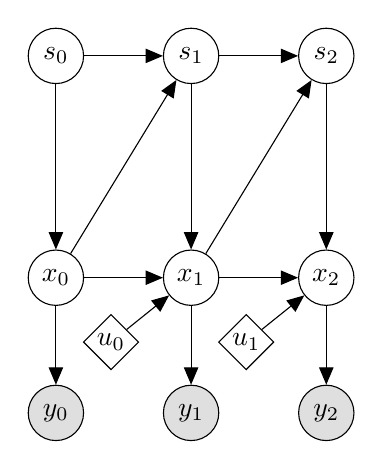
\begin{tikzpicture}

  % Define nodes
  \node[obs] (ya) {$y_{0}$};
  \node[obs, right=of ya] (yb) {$y_{1}$};
  \node[obs, right=of yb] (yc) {$y_{2}$};
  \node[latent, above=of ya]  (xa) {$x_{0}$};
  \node[latent, above=of yb, right=of xa]  (xb) {$x_{1}$};
  \node[latent, above=of yc, right=of xb]  (xc) {$x_{2}$};
  \node[det, below=of xa, xshift=0.7cm, yshift=0.9cm] (da) {$u_{0}$};
  \node[det, below=of xb, xshift=0.7cm, yshift=0.9cm] (db) {$u_{1}$};
  \node[latent, above=of xa, yshift=1.1cm] (sa) {$s_{0}$};
  \node[latent, above=of xb, yshift=1.1cm] (sb) {$s_{1}$};
  \node[latent, above=of xc, yshift=1.1cm] (sc) {$s_{2}$};
  
  % Connect the nodes
  \edge {da} {xb};
  \edge {db} {xc};
  \edge {xa} {ya};
  \edge {xb} {yb};
  \edge {xc} {yc};
  \edge {xa} {xb};
  \edge {xb} {xc};
  \edge {sa} {sb};
  \edge {sb} {sc};
  \edge {sa} {xa};
  \edge {sb} {xb};
  \edge {sc} {xc};
  \edge {xa} {sb};
  \edge {xb} {sc};
    
\end{tikzpicture}
\caption{Augmented Switching Kalman filter graphical model.}
\label{fig_gm_augmented}
\end{figure}
Using this model it is possible to specify the effect the state variables $(x_0,x_1,...)$ have on the switching variables $(s_0, s_1,...)$. Plausibly this could ameliorate the problem however, since this would require that we modify the graphical model we leave this for future work.  

\documentclass[../masters.tex]{subfiles}

\begin{document}
\graphicspath{{./imgs/}{../imgs/}} %look for images

\section{Conclusion}
Lets conclude things.


%\bibliographystyle{plain}
%\bibliography{research}

\end{document}

%References
\newpage
\bibliographystyle{plain}
\bibliography{./docs/research}

\end{document}